% !Mode:: "TeX:UTF-8"
%!TEX program  = xelatex

\documentclass[bwprint]{gmcmthesis}
\usepackage{moreverb,epsfig,subfigure}

\title{对恐怖袭击事件记录数据的量化分析}
\baominghao{18107050029} %参赛队号
\schoolname{西安石油大学}%学校名称
\membera{张鑫} %队员A
\memberb{任萌} %队员B
\memberc{成怡瑶} %队员C
\begin{document}

 %生成标题
 \maketitle

 %填写摘要
\begin{abstract}

本文通过对GTD数据集进行统计,可视化,聚类分析,分类,
以及数据预测分析来分析恐怖袭击事件的危害性,并对其危害性进行分级。
首先对数据进行可视化,我们发现,
爆炸/轰炸这一类型恐怖事件在近年来的恐怖事件中最为常见。
近二十年的恐怖事件大都发生在中东和北非。
时间上可以看到2015年为恐怖事件大幅增加的一年。
不同的国家,不同国籍,其恐怖事件类型也会不太一样。
首先,针对问题一,题目中讲到通常情况下的恐怖事件分级一般会采用主观方法,
但是,当我们学习了数学建模,学习了数据挖掘技术之后,
我们就知道,无论我们要怎么样评判一个事件的标准,
都需要由科学或者理论的依据。
从而,根据查阅参考文献,和相关官方资料,
发现影响恐怖袭击案件危害性的因素有很多,
我们就将GTD数据库中的对应特征变量拿出来,
通过高斯混合聚类算法对数据中的恐怖事件进行了聚类,
通过聚类结果对其加权并分为五个等级,

然后,针对问题二,因为是要对未知犯罪团伙或个人进行嫌疑人排序,
那么我们认为这个问题可以作为一个分类问题来处理,
对于未知犯罪团伙或个人的事件进行了分类和相似度计算(欧氏距离)。
从而找到距离未知案件最近的五个疑似犯罪团伙。
最后,问题三,我们将其刻画为一个预测问题,
通过预测算法对未来反恐态势从恐怖袭击事件发生的主要原因、
时空特性、蔓延特性、级别分布规律等进行了分析,并得到了一些预测结果。
以上三个步骤也贯穿了整个数据分析的过程。
同时,还有一些数据的可视化分析,来帮助我们更好地认识数据,
从而更有利于判断后面的分类、聚类和预测结果的正确性。

GTD数据库是非常有价值的,
不仅仅可以通过其进行聚类,分类和预测,
还可以通过该数据集来判断犯罪团伙的作案动机,
作案手段,以及作案心里,着不仅仅使得我们的建模更加有意义,
也能使得社会有更进一步的发展。

\keywords{恐怖袭击\quad  量化分析\quad   数据可视化\quad  聚类分析}
\end{abstract}

\pagestyle{plain}

%目录 不推荐加
\tableofcontents


\newpage
\section{问题重述}

\subsection{引言}

恐怖袭击是指极端分子或组织人为制造的、
针对但不仅限于平民\cite{Kaye2008More}及民用设施的、
不符合国际道义的攻击行为,
它不仅具有极大的杀伤力,
能直接造成巨大的人员伤亡和财产损失,
而且还给人们带来巨大的心理压力,
造成社会一定程度的动荡不安,
妨碍正常的工作与生活秩序,
进而极大的阻碍经济的发展。
恐怖主义是人类的共同威胁,
打击恐怖主义是每个国家应该承担的责任。
对恐怖袭击事件相关数据的深入分析有助于加深人们对恐怖主义的认识,
为反恐防恐提供有价值的信息支持。

全球恐怖主义数据库(GTD)中记录了1998-2017年世界上发生的恐怖袭击事件。
数据显示恐怖袭击事件在全球一直发生着并成为全球的不稳定因素,
也有许多国家和地区采取了一系列政策。
但是恐怖袭击是一种突发事件,
其不确定性将对今后事件态势的发展的预估造成很大的影响。
因此,
如何表达数据本身及其包含的不确定性,
成为恐怖袭击数据分析中的重要问题。

其中恐怖袭击采用的武器也可以被分为十几类,
生化武器,化学武器,放射性武器,核武器,
轻武器,爆炸物/炸药/炸弹,假武器,燃烧武器,
致乱武器,交通工具\cite{Lucci2006Civilian},
破坏设备\cite{Ackerman2010WMD}
以及其他未知武器。

\cite{PGNN2018}是2018年研究人员在新奥尔良举办的人工智能、
道德与社会(AIES)会议上发表的最新成果。
在美国,当有人殴打行人、抢劫商店或冷血杀人时,
警察需要派遣一个特别的执法小组,
调查此人是否隶属于某个犯罪团伙成员。
而这篇文章提出一种新的算法来试图自动识别团伙犯罪。
可见,随着科学技术的进步,大数据技术的逐步发展,
很多事件我们都可以从中发现规律,
使得恐怖事件得到控制。
那么本文就通过GTD数据库数据来做分析。
\cite{王锂达2016挖掘恐怖组织行为模式}
利用FP-Growth的滑动时间窗口衰减的因果关联建模算法,
通过恐怖组织袭击的武器、地点、袭击目标进行了行为模式挖掘。
从而对恐怖组织活动规律有了一定的预测。

\subsection{研究问题}

已知数据变量总共九类:
GTD的标志号和日期、
事件信息、
事件发生的地点、
攻击信息、
武器信息、
目标/受害者信息、
凶手信息、
伤亡和后果、
附加信息和来源。
通过这些信息来对恐怖袭击事件的发生进行深入分析,
从而对反恐防恐提供有价值的信息支持。

\subsubsection{问题一:依据危害性对恐怖袭击事件分级}

对灾难性事件比如地震、交通事故、气象灾害等等进行分级是社会管理中的重要工作。
通常的分级一般采用主观方法,
由权威组织或部门选择若干个主要指标,
强制规定分级标准,
如我国《道路交通事故处理办法》第六条规定的交通事故等级划分标准,
主要按照人员伤亡和经济损失程度划分。
但恐怖袭击事件的危害性不仅取决于人员伤亡和经济损失这两个方面,
还与发生的时机、地域、针对的对象等等诸多因素有关,
因而采用上述分级方法难以
形成统一标准。
依据GTD数据库中的有关信息,
结合现代信息处理技术,
借助数学建模方法建立基于数据分析的量化分级模型,
将GTD中给出的事件按危害程度从高到低分为一至五级,
列出近二十年来危害程度最高的十大恐怖袭击事件,
并给出表1中事件的分级。


\begin{table}
\centering
\caption{典型事件危害级别}
\begin{tabular}{|c|c|}
  \hline
  % after \\: \hline or \cline{col1-col2} \cline{col3-col4} ...
  事件编号 & 危害级别 \\
  \hline
  200108110012 & 2  \\
  \hline
  200511180002 & 2 \\
  \hline
  200901170021 & 2 \\
  \hline
  201402110015 & 2 \\
  \hline
  201405010071 & 2 \\
  \hline
  201411070002 & 1  \\
  \hline
  201412160041 & 2  \\
  \hline
  201508010015 & 5  \\
  \hline
  201705080012 & 2  \\
  \hline
\end{tabular}
\end{table}


\subsubsection{问题二:依据事件特征发现恐怖袭击事件制造者}

GTD数据库中有多起恐怖袭击事件尚未确定作案者。
如果将可能是同一个恐怖组织或个人在不同时间、
不同地点多次作案的若干案件串联起来统一组织侦査,
有助于提高破案效率,
有利于尽早发现新生或者隐藏的恐怖分子。请你们针对在
2015、2016 年度发生的、尚未有组织或个人宣称负责的恐怖袭击事件,
运用数学建模方法寻找上述可能性,
即将可能是同一个恐怖组织或个人在不同时间、不同地点多次作案的若干案件归为一类,
对应的未知作案组织或个人标记不同的代号,
并按该组织或个人的危害性从大到小选出其中的前5个,
记为1号-5号。
再对表2列出的恐袭事件,
按嫌疑程度对5个嫌疑人排序,
并将结果填入下表
(表中样例的意思是:
对事件编号为XX的事件,
3号的嫌疑最大,其次是4号,
最后是5号),
如果认为某嫌疑人关系不大,
也可以保留空格。

\begin{table}
\centering
\caption{恐怖分子关于典型事件的嫌疑度}
\resizebox{\textwidth}{35mm}{
\begin{tabular}{|c|c|c|c|c|c|}
  \hline
  % after \\: \hline or \cline{col1-col2} \cline{col3-col4} ...
  事件编号
  & 1号嫌疑人
  & 2号嫌疑人
  & 3号嫌疑人
  & 4号嫌疑人
  & 5号嫌疑人
  \\
  \hline
  201701090031
  & Islamic State of Iraq and the Levant (ISIL)
  & Al-Qaida in the Arabian Peninsula (AQAP)
  & Abu Sayyaf Group (ASG)
  & Abdul Ghani Kikli Militia
  & Abu Amarah Battalion
  \\
  \hline
  201702210037
  & Islamic State of Iraq and the Levant (ISIL)
  & Abu Sayyaf Group (ASG)
  & Abbala extremists
  & Abu Sayyaf Group (ASG)
  & Abdul Ghani Kikli Militia
  \\
  \hline
  201703120023
  & Boko Haram
  & Abu Sayyaf Group (ASG)
  & Abbala extremists
  & Abdul Ghani Kikli Militia
  & Abu Amarah Battalion
  \\
  \hline
  201705050009
  & Taliban
  & Abu Sayyaf Group (ASG)
  & Abbala extremists
  & Abdul Ghani Kikli Militia
  & Abu Amarah Battalion
  \\
  \hline
  201705050010
  & Taliban
  & Abu Sayyaf Group (ASG)
  & Abbala extremists
  & Abdul Ghani Kikli Militia
  & Abu Amarah Battalion
  \\
  \hline
  201707010028
  & Maoists
  & Abu Sayyaf Group (ASG)
  & Abbala extremists
  & Abdul Ghani Kikli Militia
  & Abu Amarah Battalion
  \\
  \hline
  201707020006
  & Islamic State of Iraq and the Levant (ISIL)
  & Abu Sayyaf Group (ASG)
  & Abbala extremists
  & Abdul Ghani Kikli Militia
  & Abu Amarah Battalion
  \\
  \hline
  201708110018
  & Taliban
  & Abu Sayyaf Group (ASG)
  & Abbala extremists
  & Abdul Ghani Kikli Militia
  & Abu Amarah Battalion
  \\
  \hline
  201711010006
  & Taliban
  & Abu Sayyaf Group (ASG)
  & Abbala extremists
  & Abdul Ghani Kikli Militia
  & Abu Amarah Battalion
  \\
  \hline
  201712010003
  & Islamic State of Iraq and the Levant (ISIL)
  & A'chik Matgrik Elite Force (AMEF)
  & Abbala extremists
  & Abdul Ghani Kikli Militia
  & Abu Amarah Battalion
  \\
  \hline
\end{tabular}}
\end{table}


\subsubsection{问题三:对未来反恐态势的分析}

对未来反恐态势的分析评估有助于提高反恐斗争的针对性和效率。
依据GTD数据库中的内容并结合因特网上的有关信息,
建立适当的数学模型,
研究近三年来恐怖袭击事件发生的主要原因、时空特性、蔓延特性、级别分布等规律,
进而分析研判下一年全球或某些重点地区的反恐态势,
用图/表给出你们的研究结果,
提出你们对反恐斗争的见解和建议。

\subsubsection{问题四:数据的进一步利用}

数据一还可以发挥哪些作用


\section{模型的假设}

\begin{enumerate}
  \item 数据预处理,假设某些空值属性为0,e.g. 财产损失(property);
  \item 任务一:利用机器学习聚类算法对GTD 数据库中的feature进行高斯聚类分析;
  \item 任务二:通过机器学习分类算法得到结果;
  \item 任务三:利用机器学习预测算法对未来反恐态势进行分析。
\end{enumerate}

\section{符号说明}

\begin{tabular}{cc} %eventid & nkill & nwound & property
 \hline
 \makebox[0.4\textwidth][c]{符号}	&  \makebox[0.5\textwidth][c]{意义} \\ \hline
 $\lambda_1$	    & eventid权值  \\ \hline
 $\lambda_2$	    & nkill权值  \\ \hline
 $\lambda_3$	    & nwound权值  \\ \hline
 $\lambda_4$	    & property权值 \\ \hline
 $x_1$	    & eventid属性值  \\ \hline
 $x_2$	    & nkill属性值  \\ \hline
 $x_3$	    & nwound属性值  \\ \hline
 $x_4$	    & property属性值  \\ \hline
\end{tabular}

\section{问题分析与求解}

在做任务分析之前,
我们看到了GTD数据库中共有114183个样本数据,
109个变量,
其中记录了1998~2017年发生的恐怖袭击的相关信息,
变量总共包含九类:
GTD的标志号和日期、
事件信息、
事件发生的地点、
攻击信息、
武器信息、
目标/受害者信息、
凶手信息、
伤亡和后果。

\subsection{数据可视化}

针对上面数据,
我们首先对恐怖袭击事件发生的时间,
地点(地区和国家),
死亡人数,财产损失,袭击类型,武器类型,袭击目标进行了可视化分析。
通过上面可视化分析可以得到下面的结果。
其中袭击类型分别为:
暗杀、武器袭击、轰炸/爆炸、
劫持、劫持人质(路障事件)、
劫持人质(绑架)、
设施/基础设施攻击、
徒手攻击、
未知攻击。

\begin{figure}[htbp]
    \subfigure{
        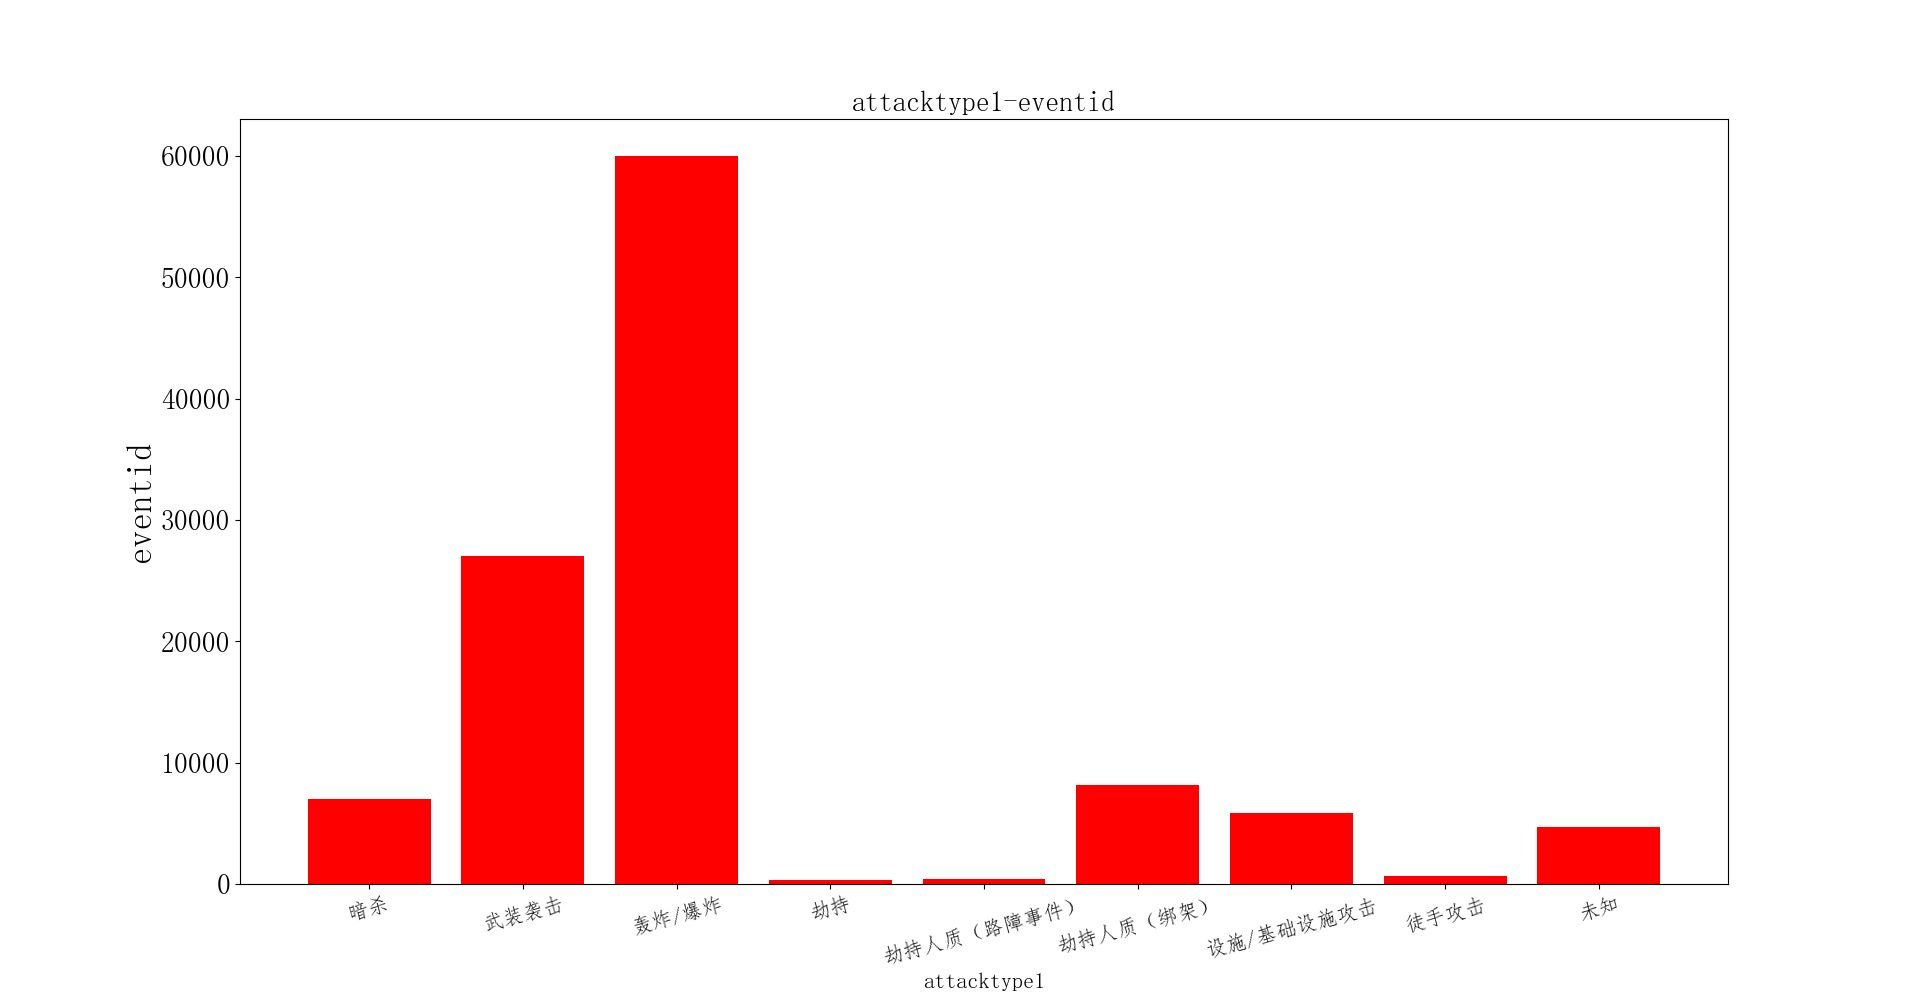
\includegraphics[width=.5\textwidth]{figures//img//Figure_1.png}

    }
    \subfigure{
        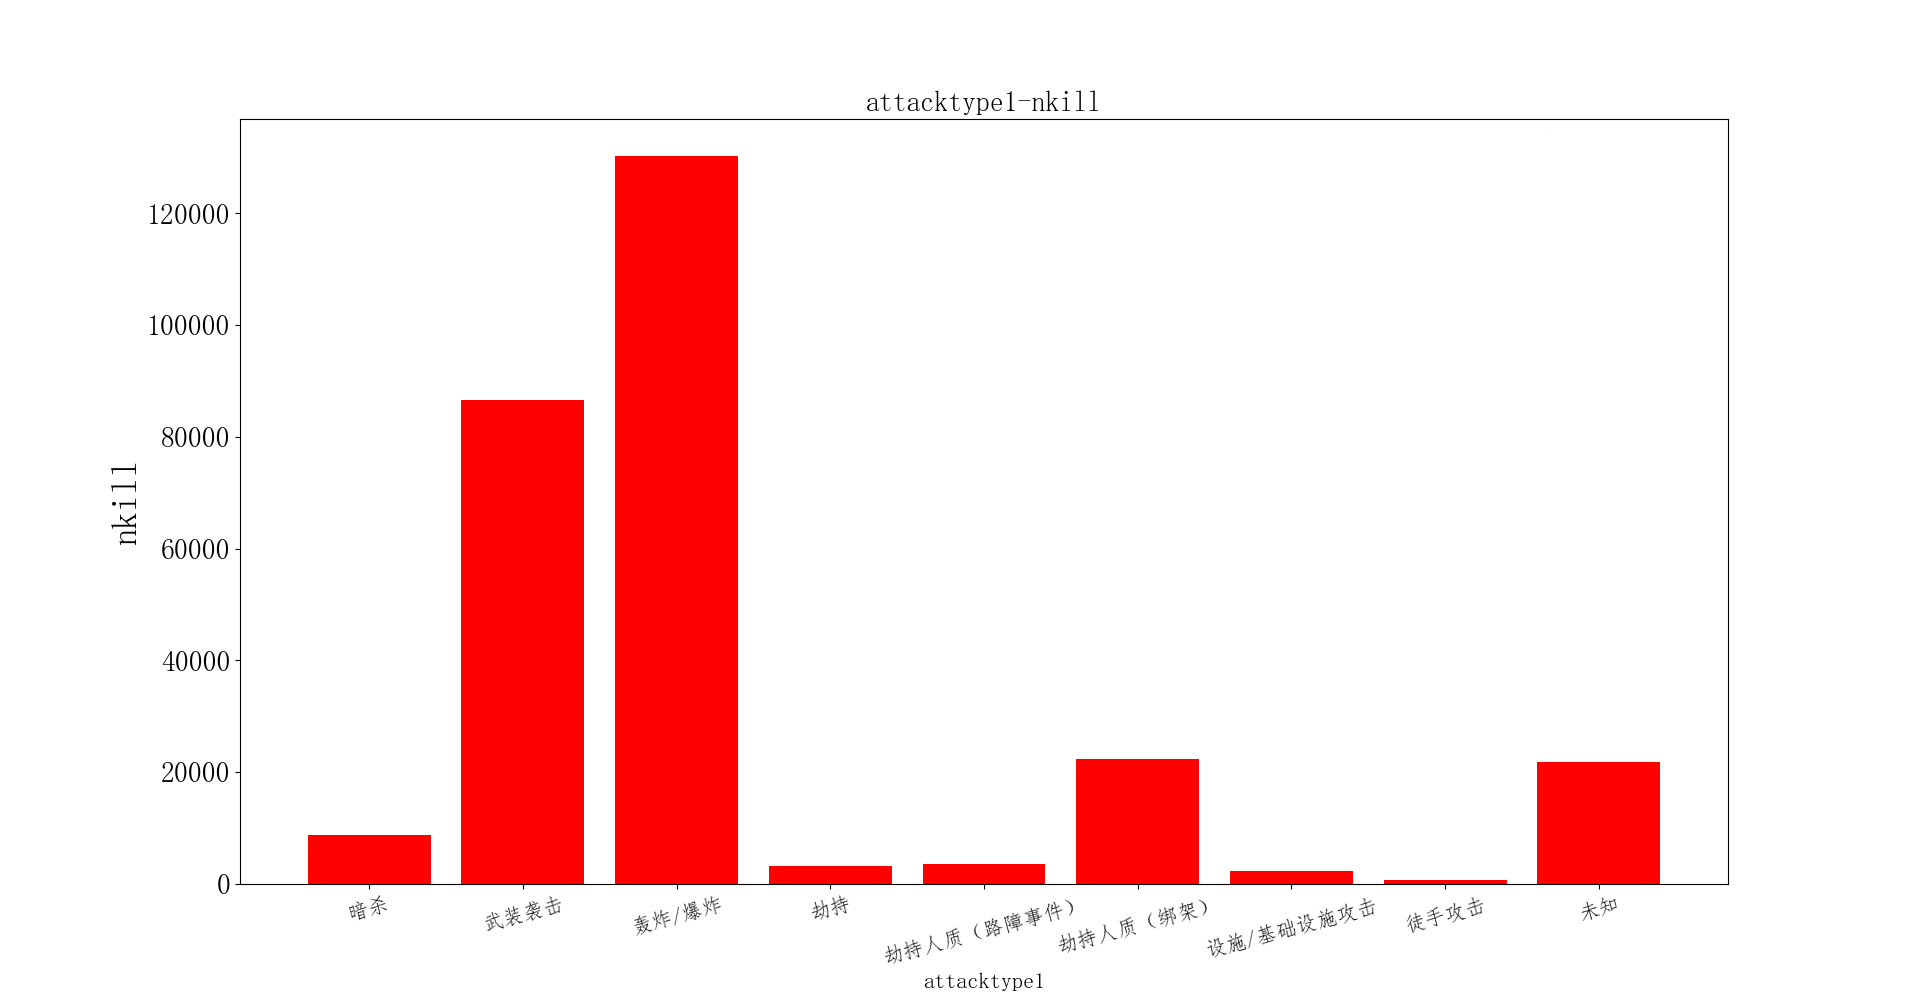
\includegraphics[width=.5\textwidth]{figures//img//Figure_1-1.png}
    }
    \subfigure{
        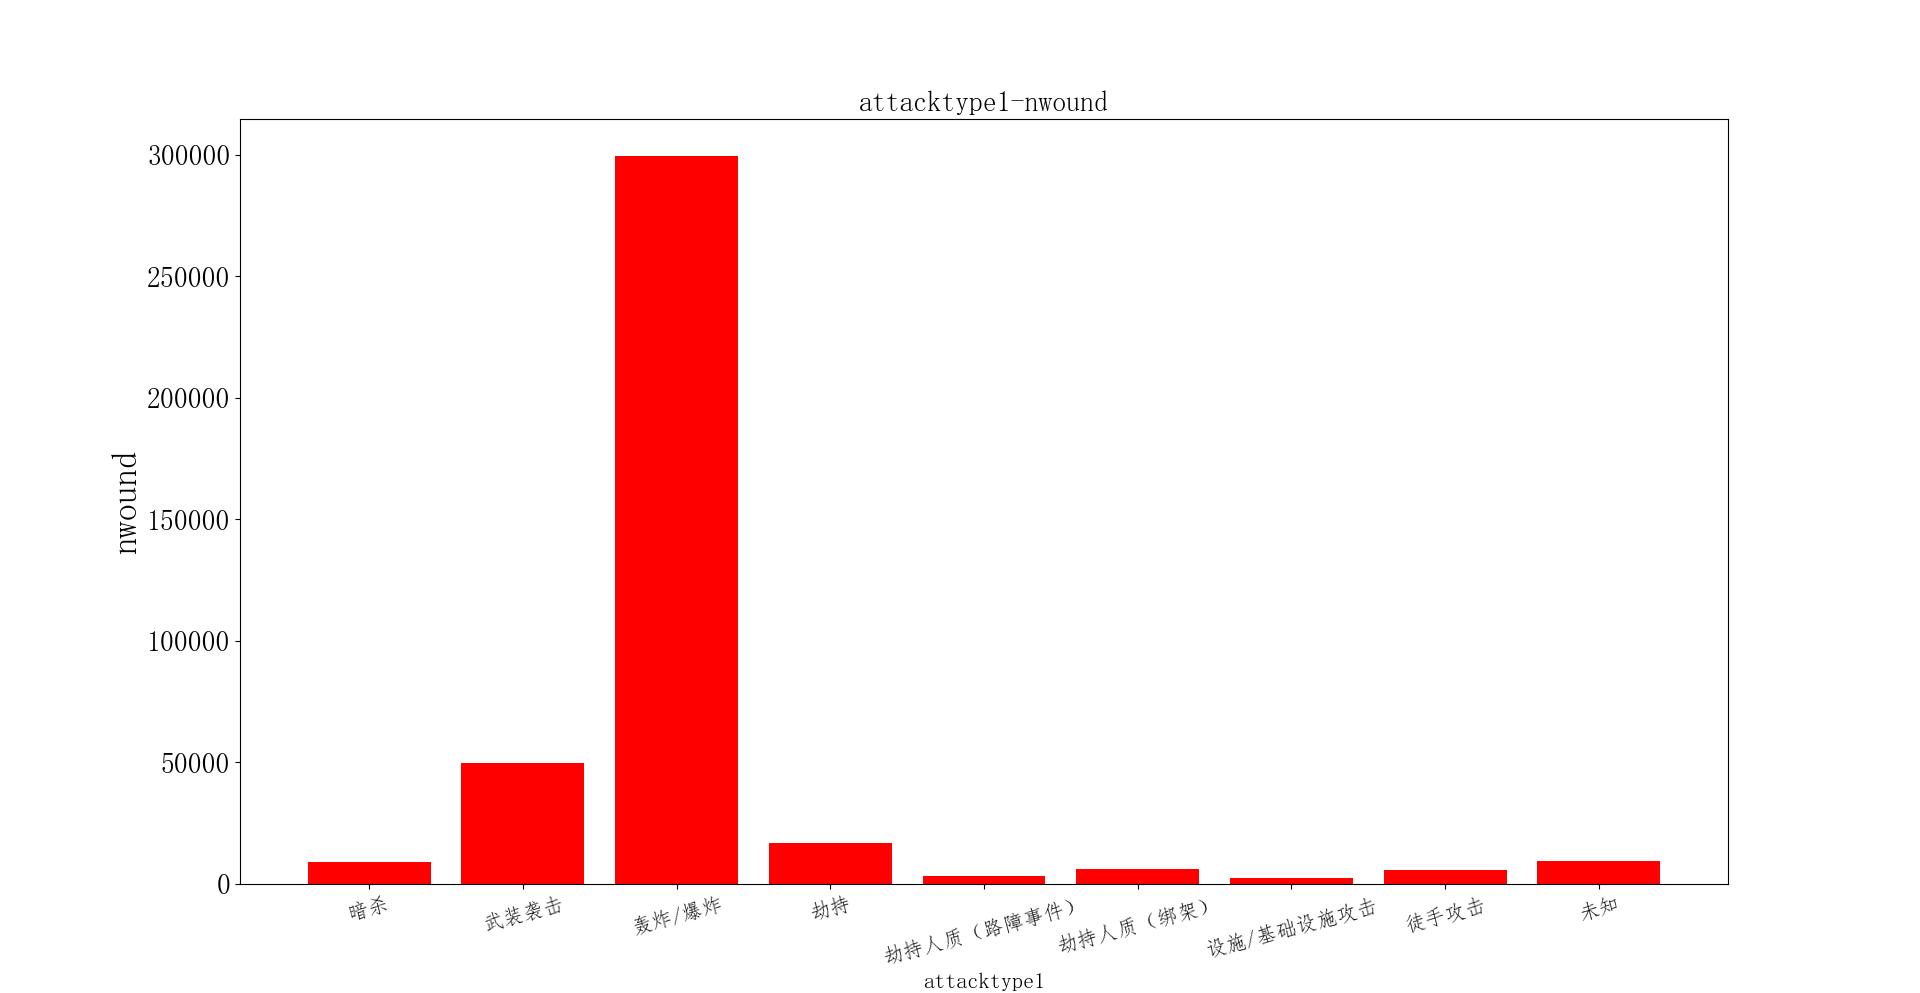
\includegraphics[width=.5\textwidth]{figures//img//Figure_1-2.png}
    }
    \subfigure{
        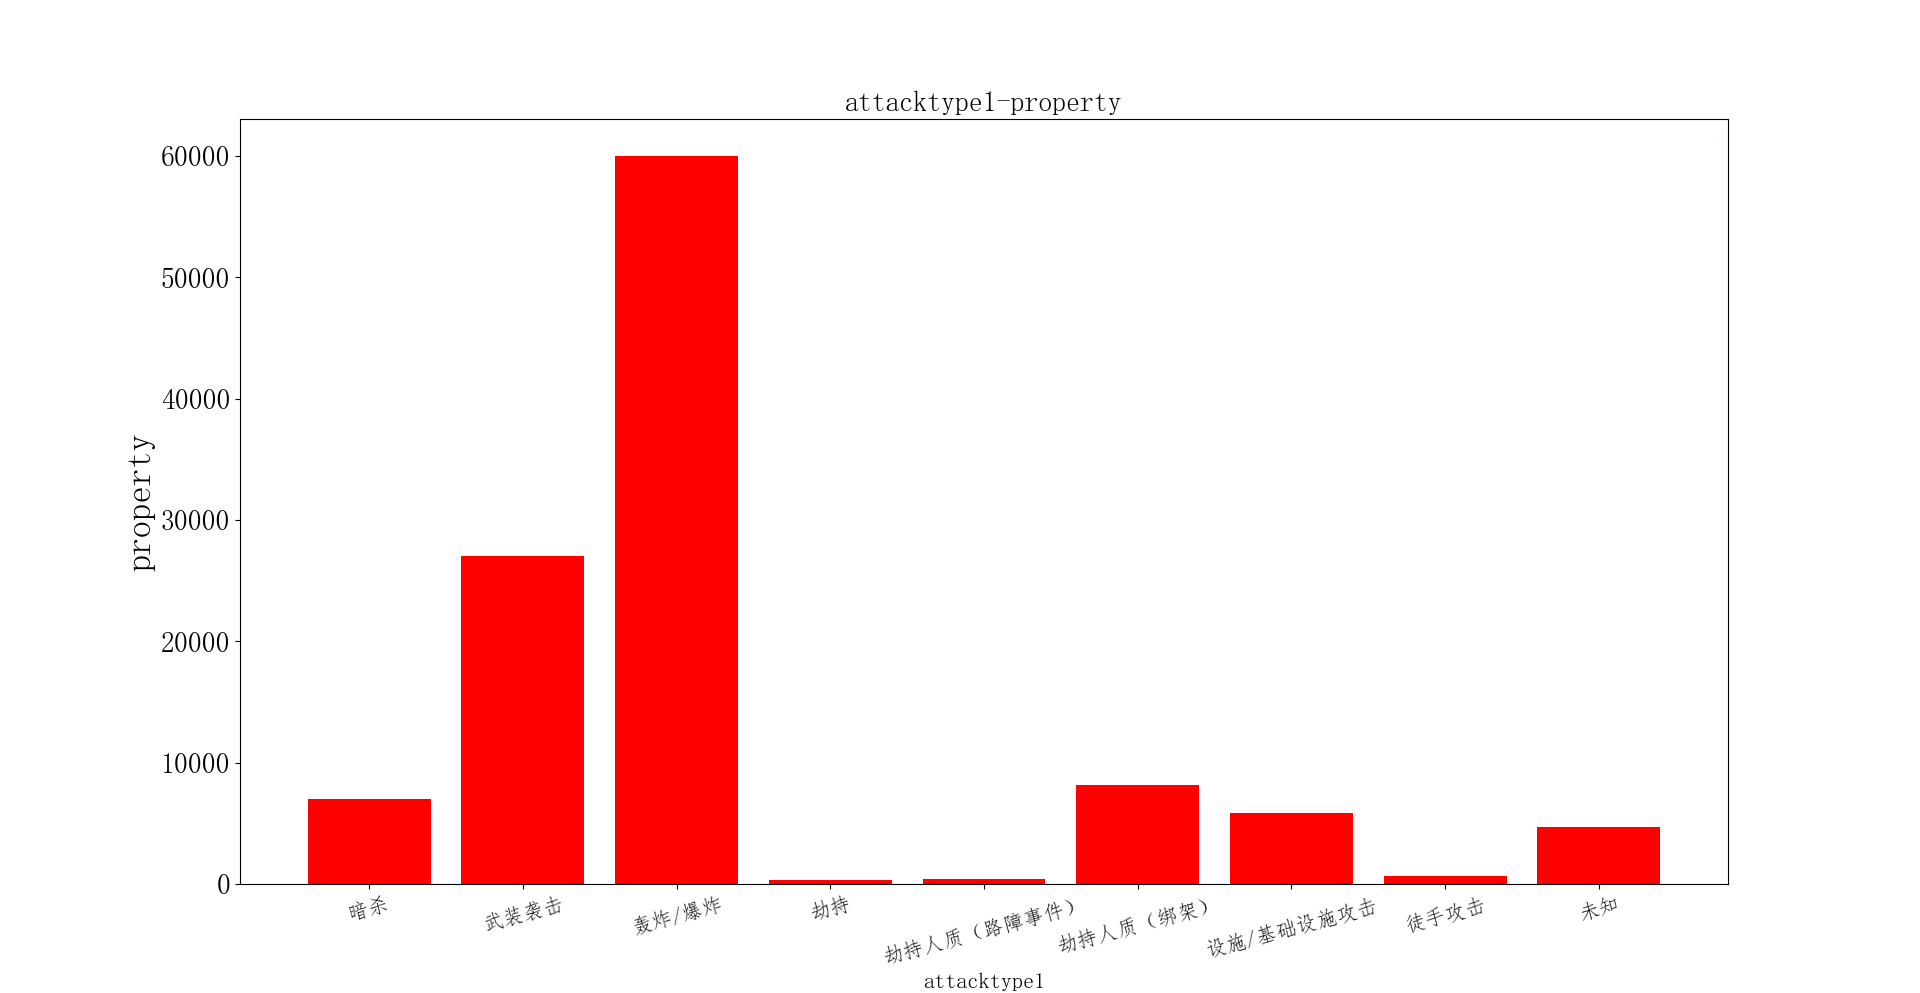
\includegraphics[width=.5\textwidth]{figures//img//Figure_1-3.png}
    }
    \caption{袭击事件发生次数、死亡人数、受伤人数和财产损失按袭击类型分布统计图}
    \label{tab:袭击类型}
\end{figure}

图\ref{tab:袭击类型}利用条形统计图对不同的袭击类型、死亡人数、
受伤人数和财产损失按袭击类型进行了统计。
从图中可以很直观的看到,
轰炸/爆炸这一类型的恐怖袭击发生最频繁。

\begin{figure}[htbp]
    \subfigure{
        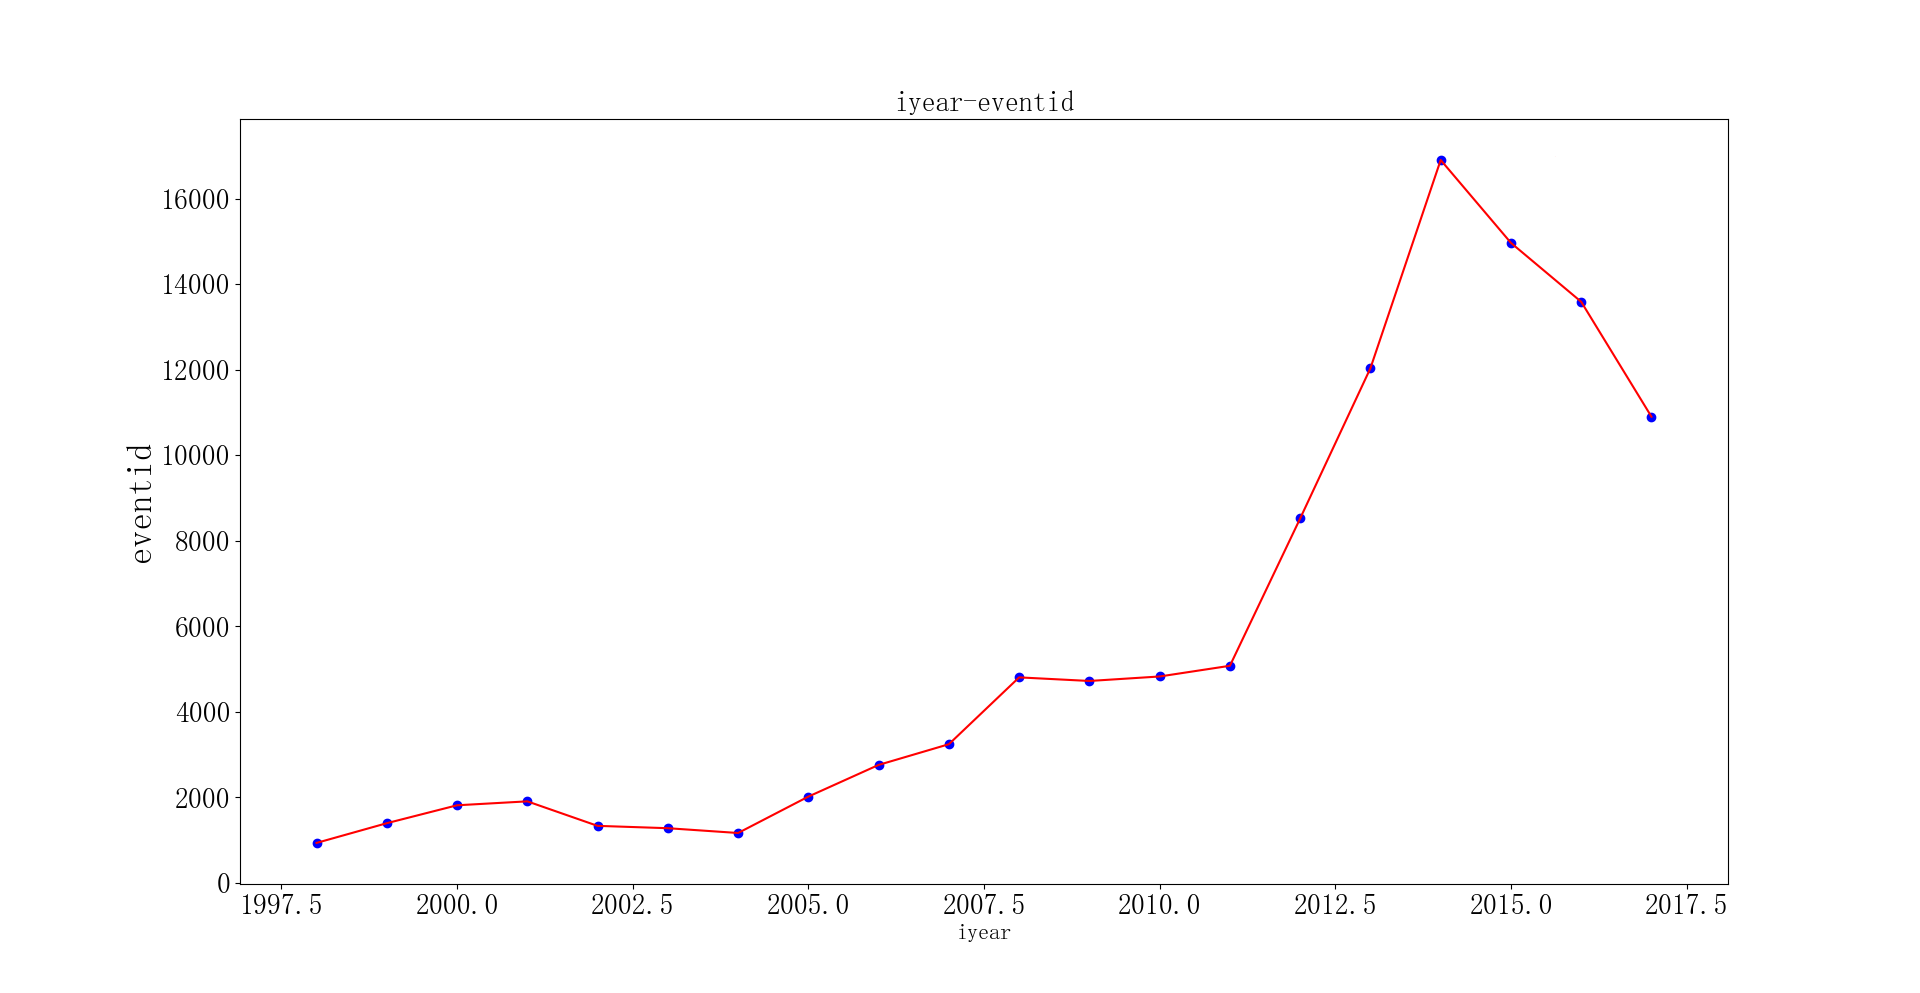
\includegraphics[width=.5\textwidth]{figures//img//Figure_1-8.png}

    }
    \subfigure{
        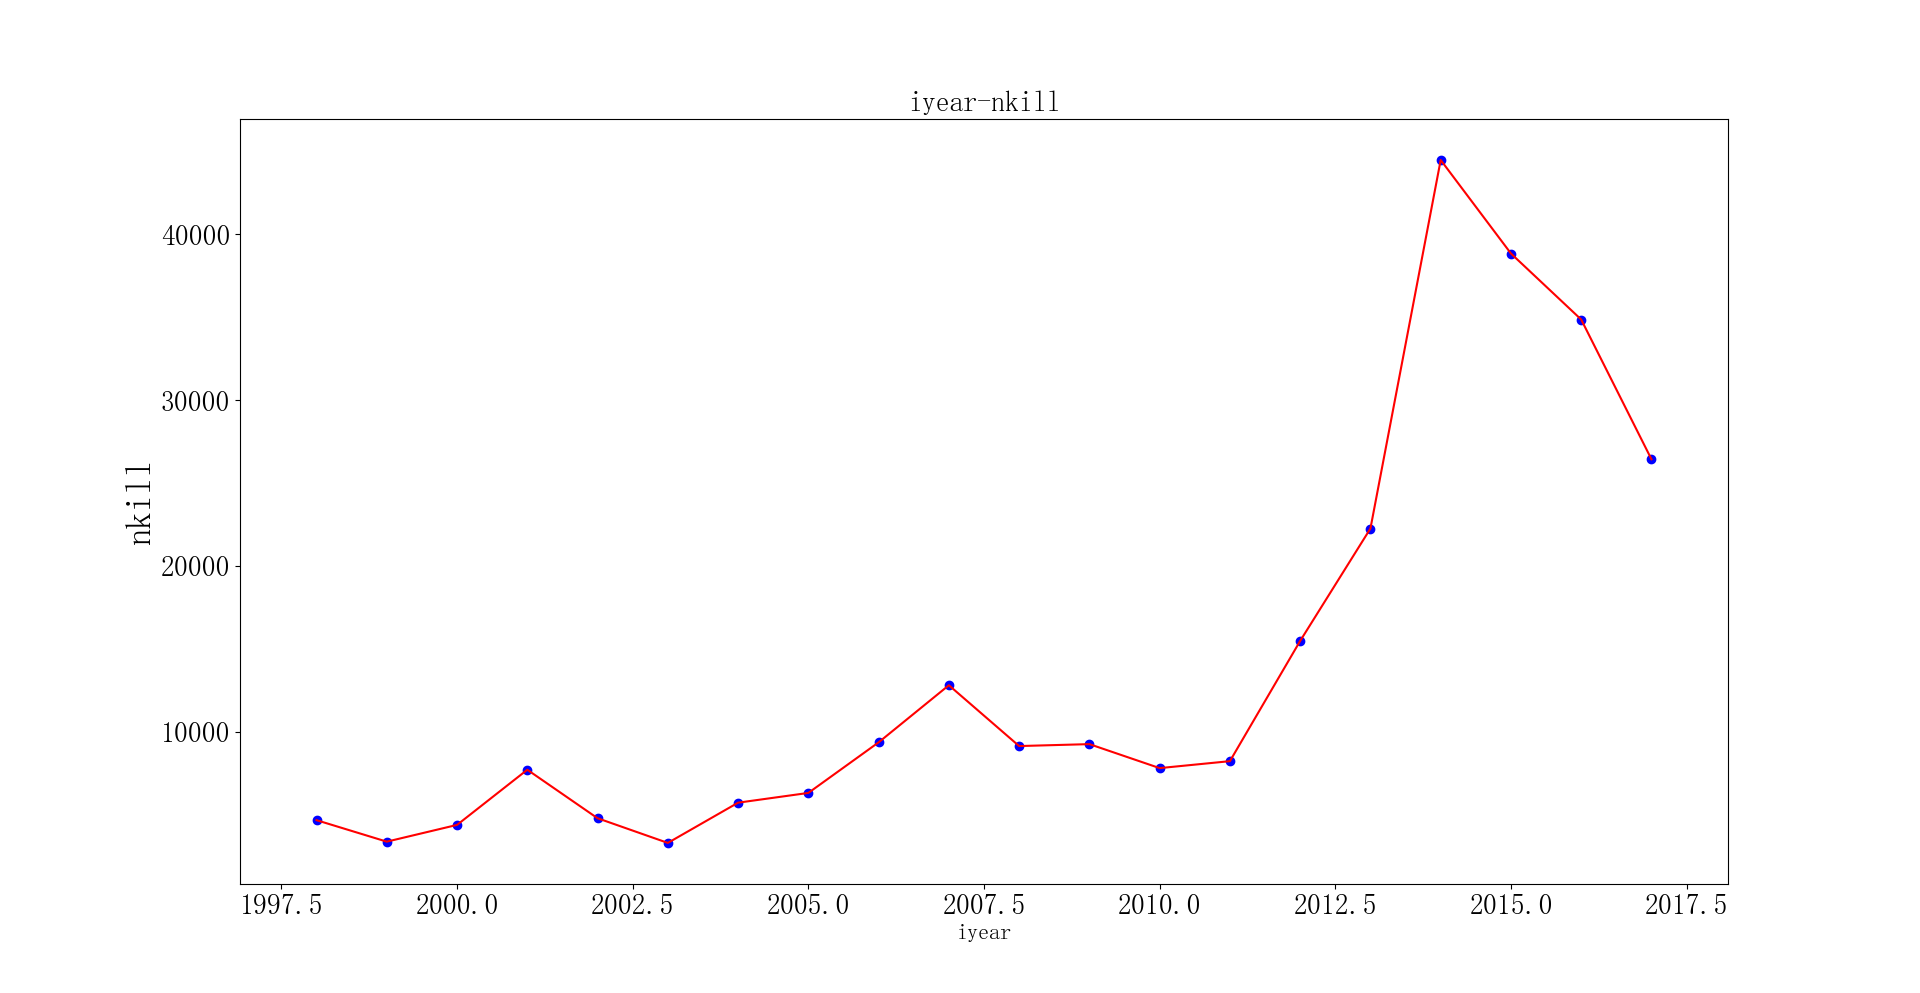
\includegraphics[width=.5\textwidth]{figures//img//Figure_1-9.png}
    }
    \subfigure{
        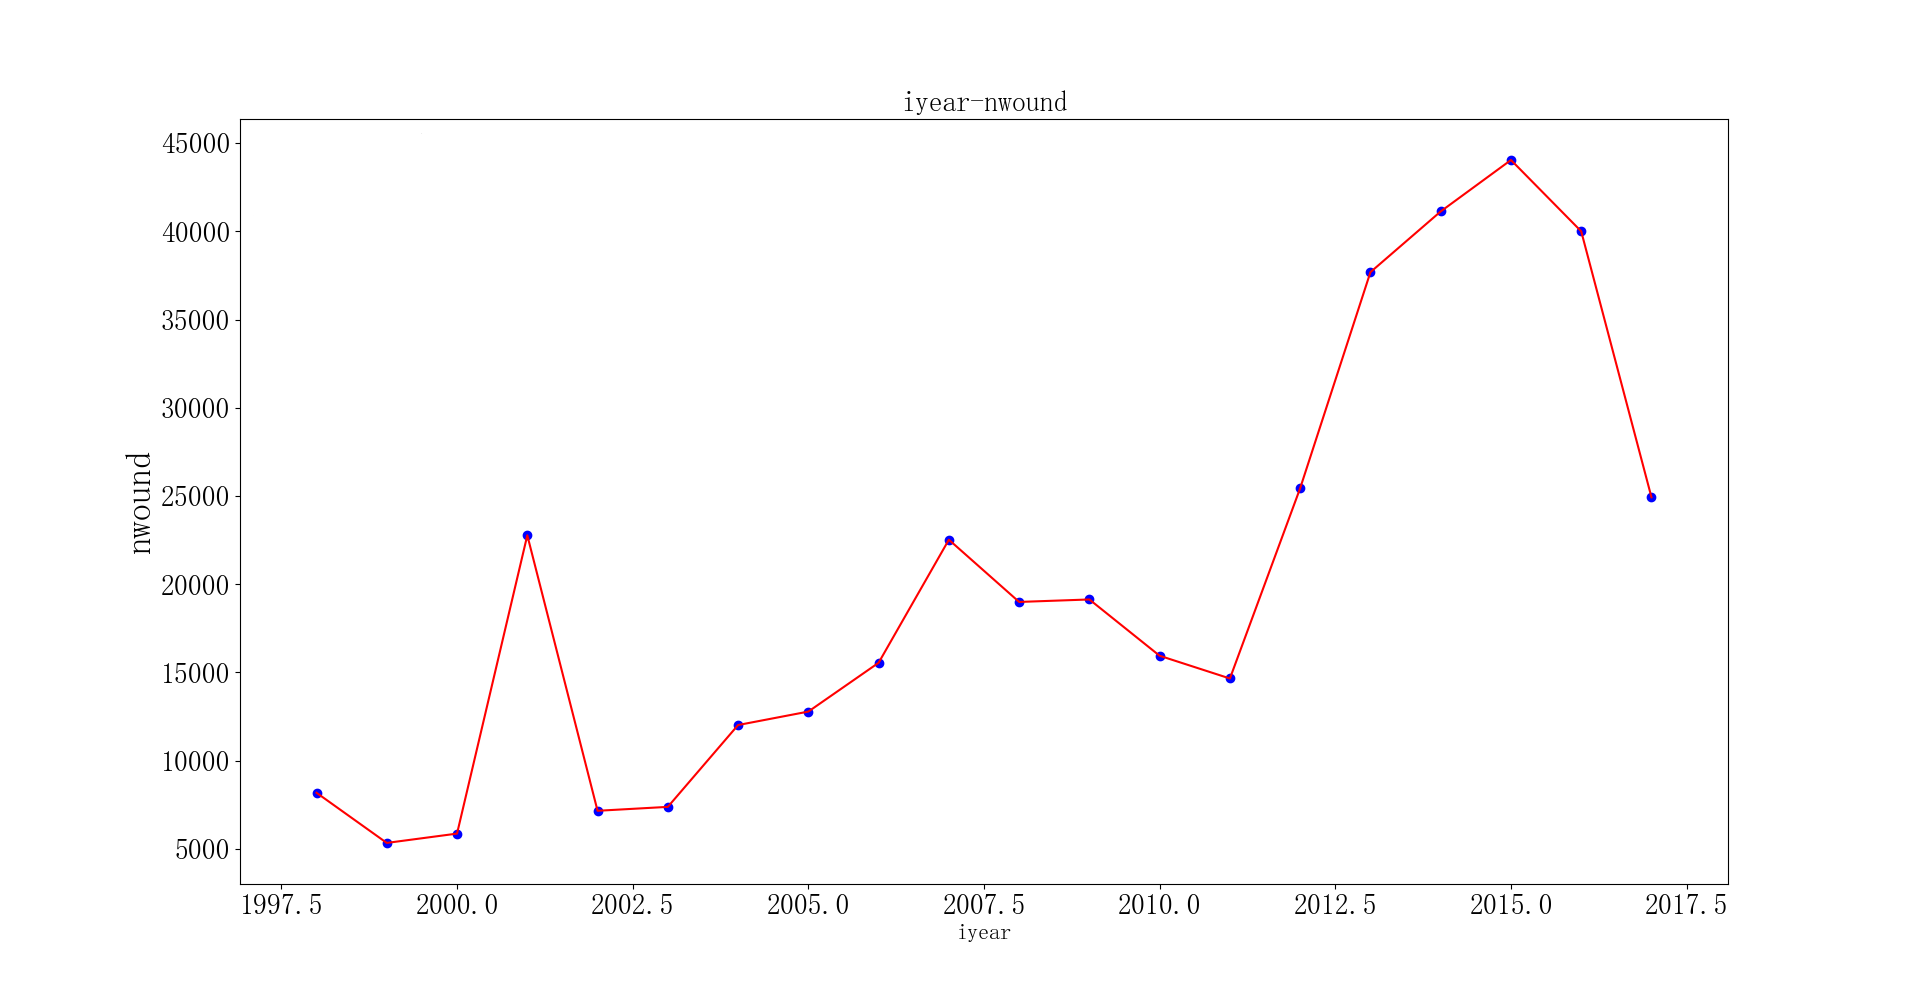
\includegraphics[width=.5\textwidth]{figures//img//Figure_1-10.png}
    }
    \subfigure{
        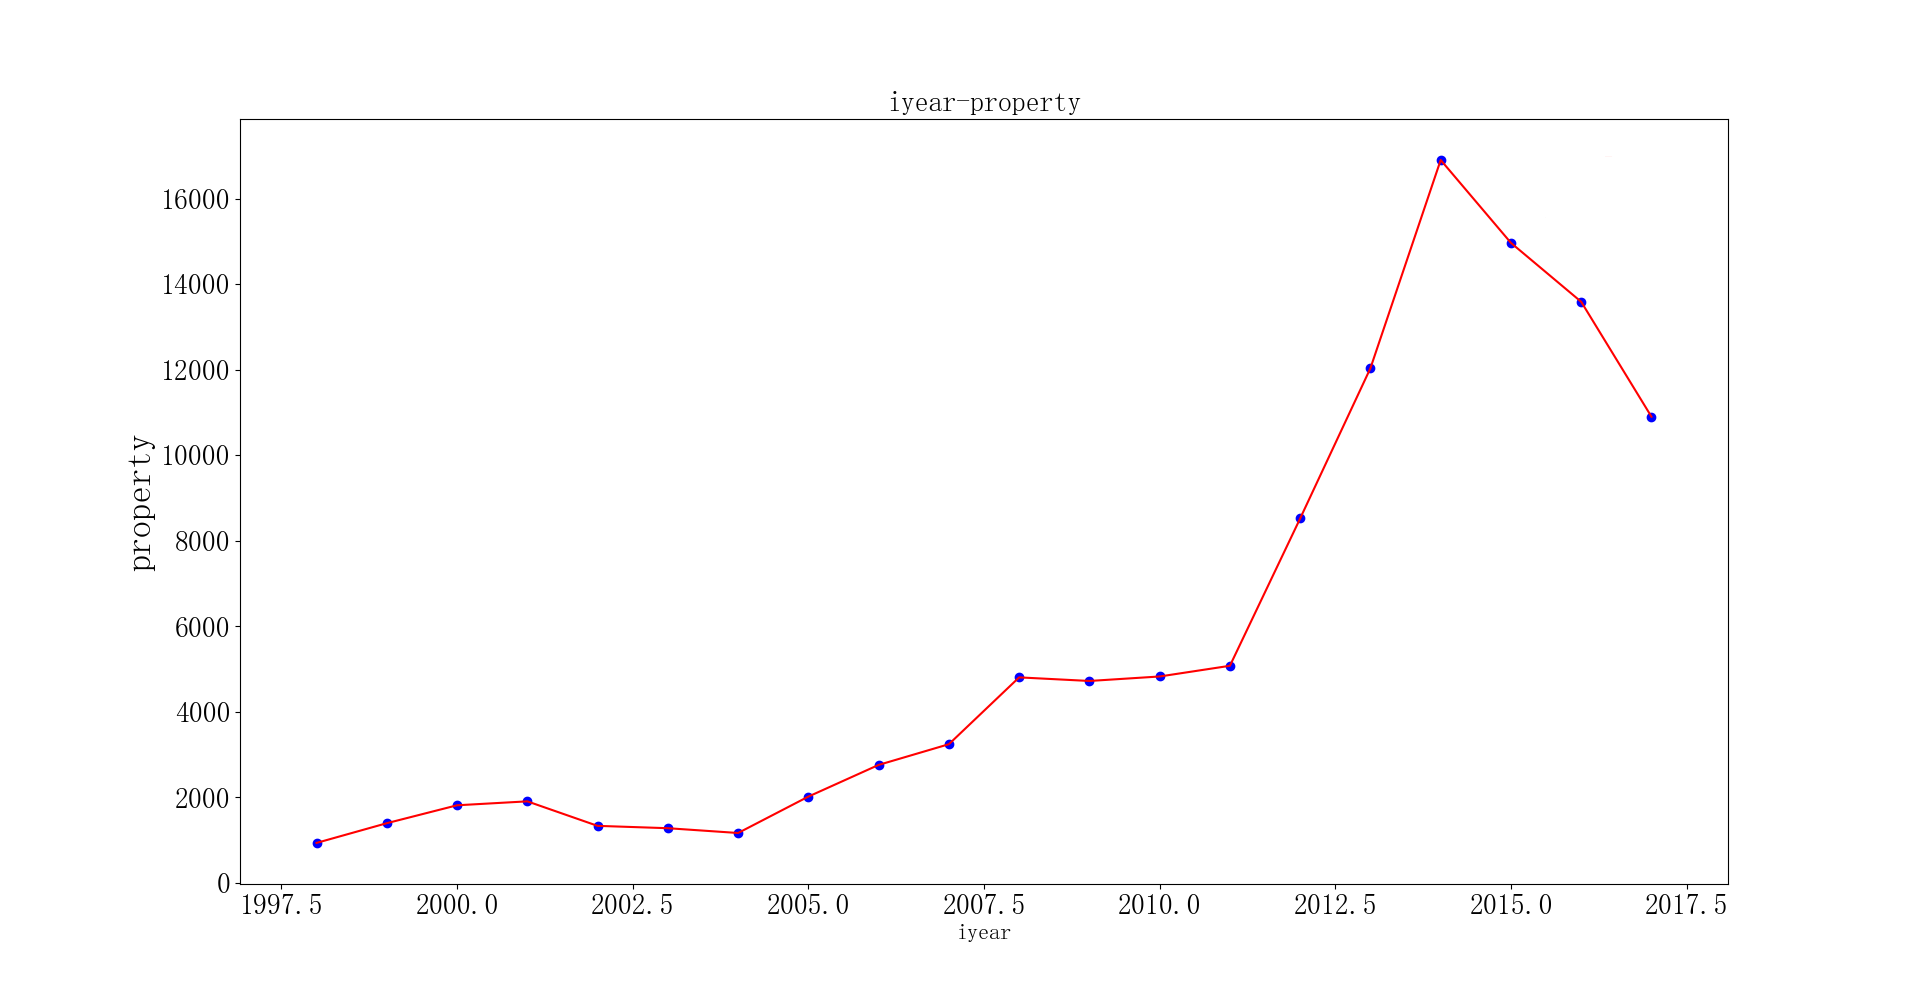
\includegraphics[width=.5\textwidth]{figures//img//Figure_1-11.png}
    }
    \caption{袭击事件发生次数、死亡人数、受伤人数和财产损失按时间分布统计图}
    \label{tab:时间分布}
\end{figure}

图\ref{tab:时间分布}利用折现图对袭击事件发生次数、
死亡人数、受伤人数和财产损失按照时间进行了统计。
可以看到2001年死亡人数有所升高,
2012~2015年期间,
恐怖袭击事件发生次数、死亡人数、受伤人数以及财产损失有大幅度的升高。

\begin{figure}[htbp]
    \subfigure{
        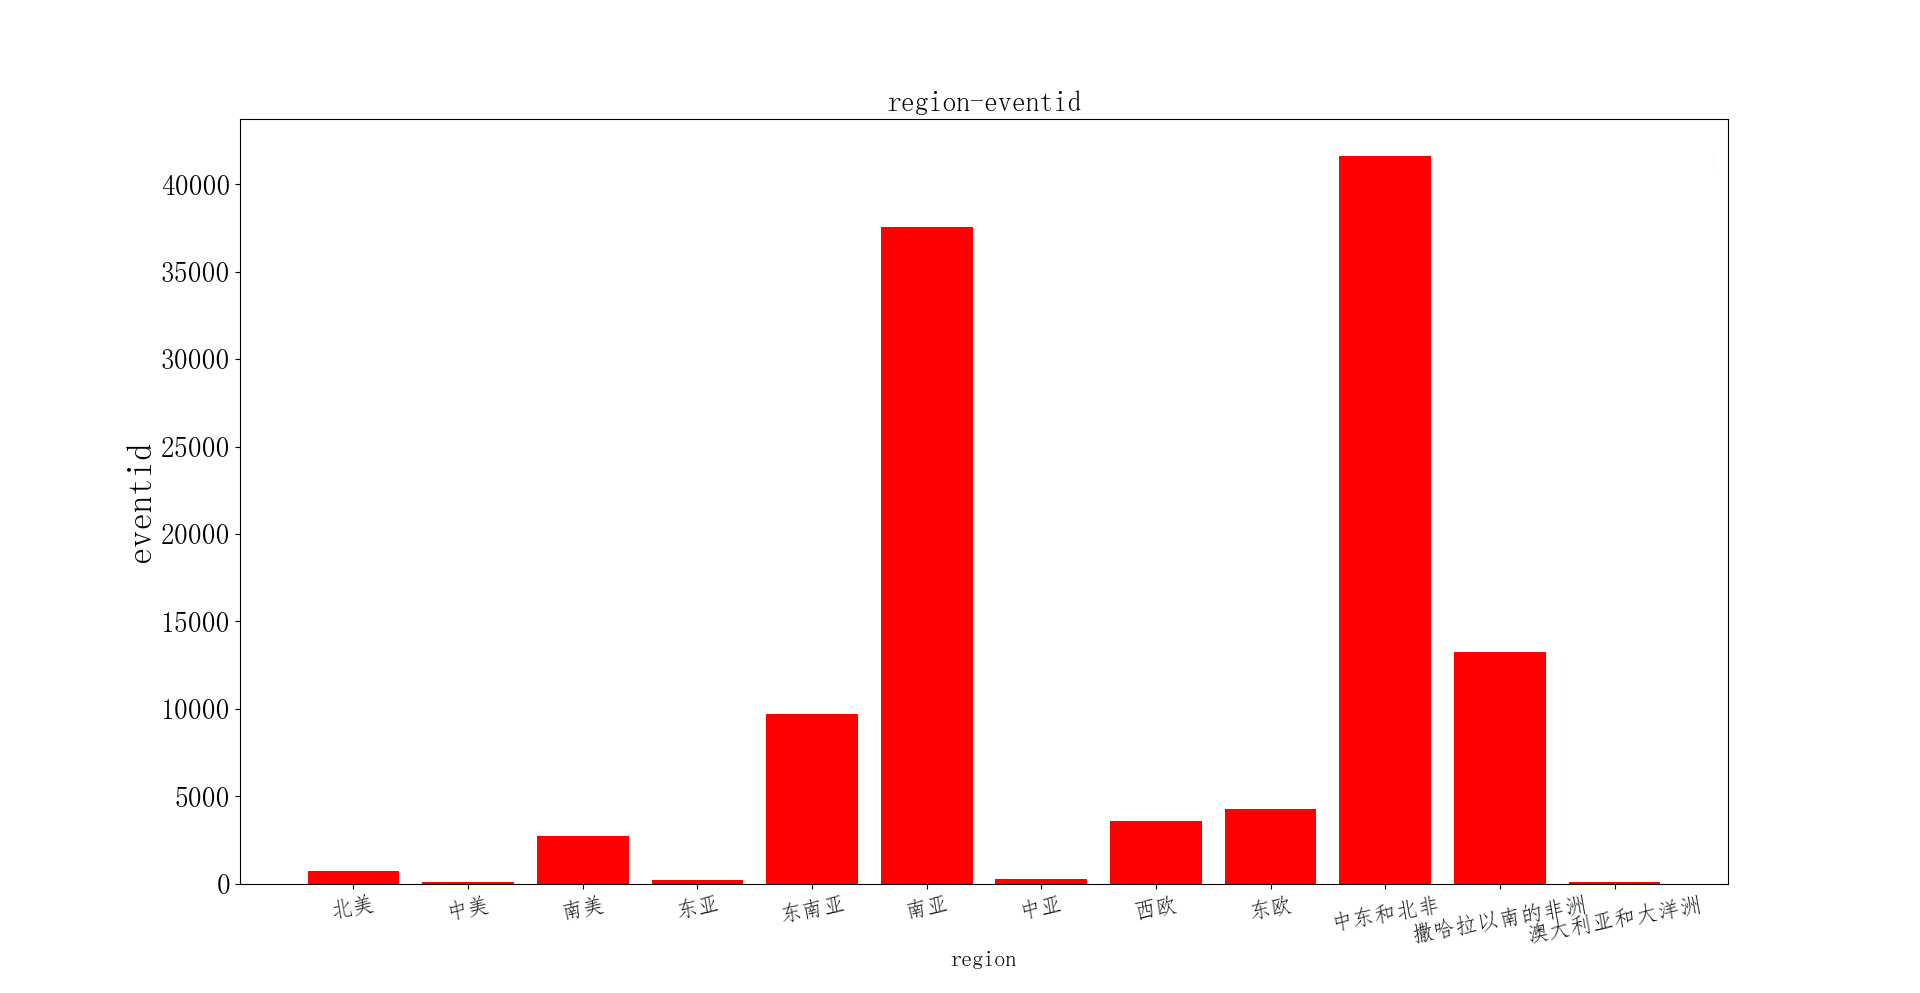
\includegraphics[width=.5\textwidth]{figures//img//Figure_1-12.png}

    }
    \subfigure{
        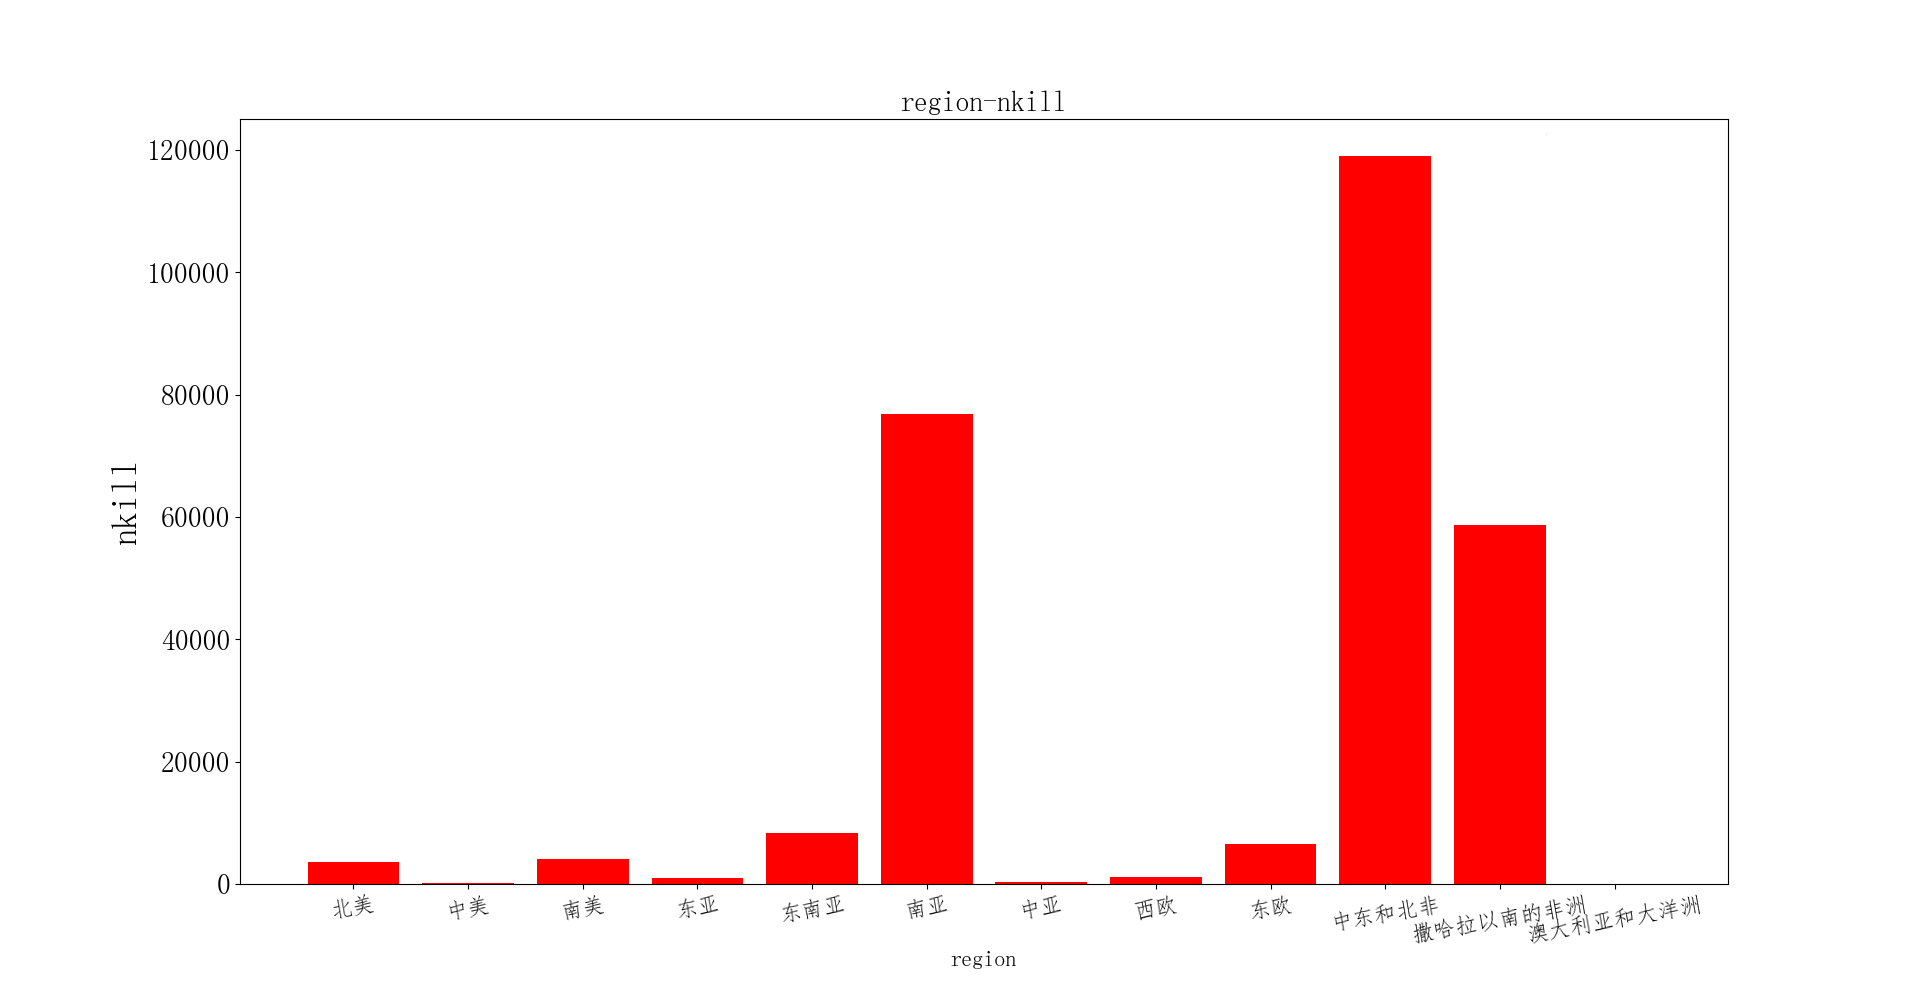
\includegraphics[width=.5\textwidth]{figures//img//Figure_1-13.png}
    }
    \subfigure{
        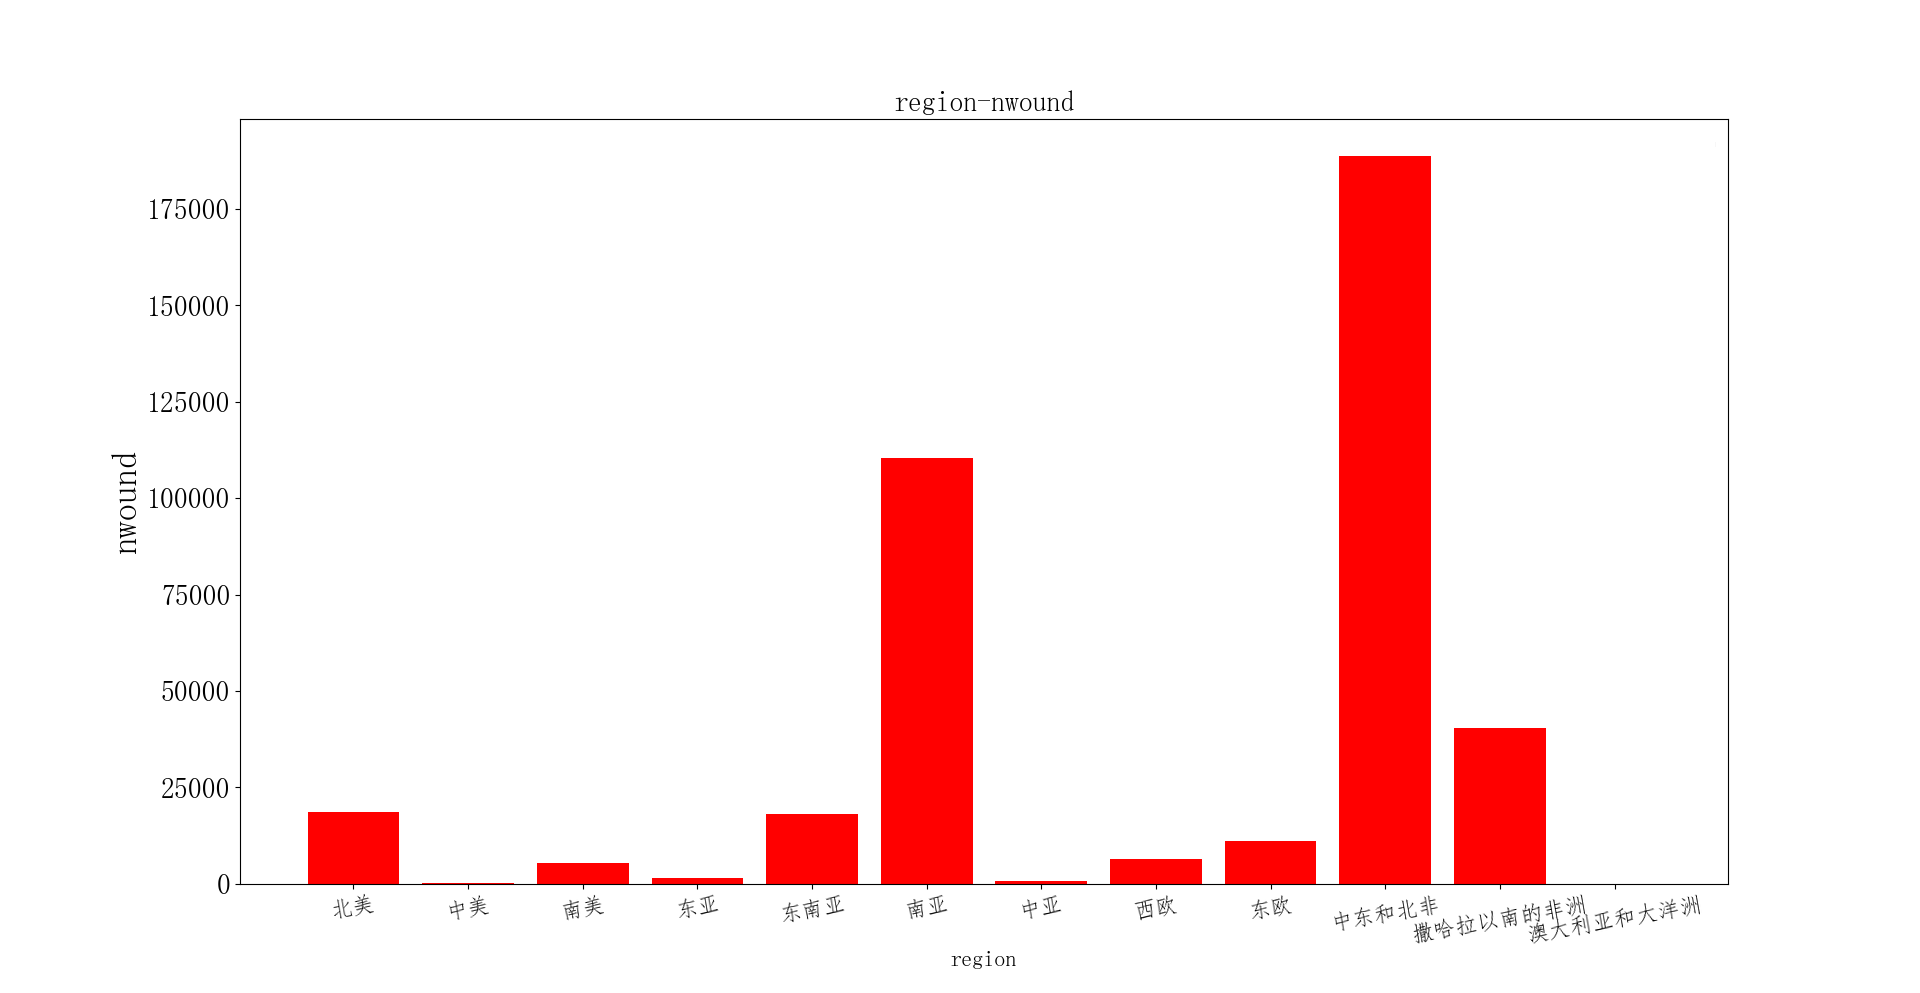
\includegraphics[width=.5\textwidth]{figures//img//Figure_1-14.png}
    }
    \subfigure{
        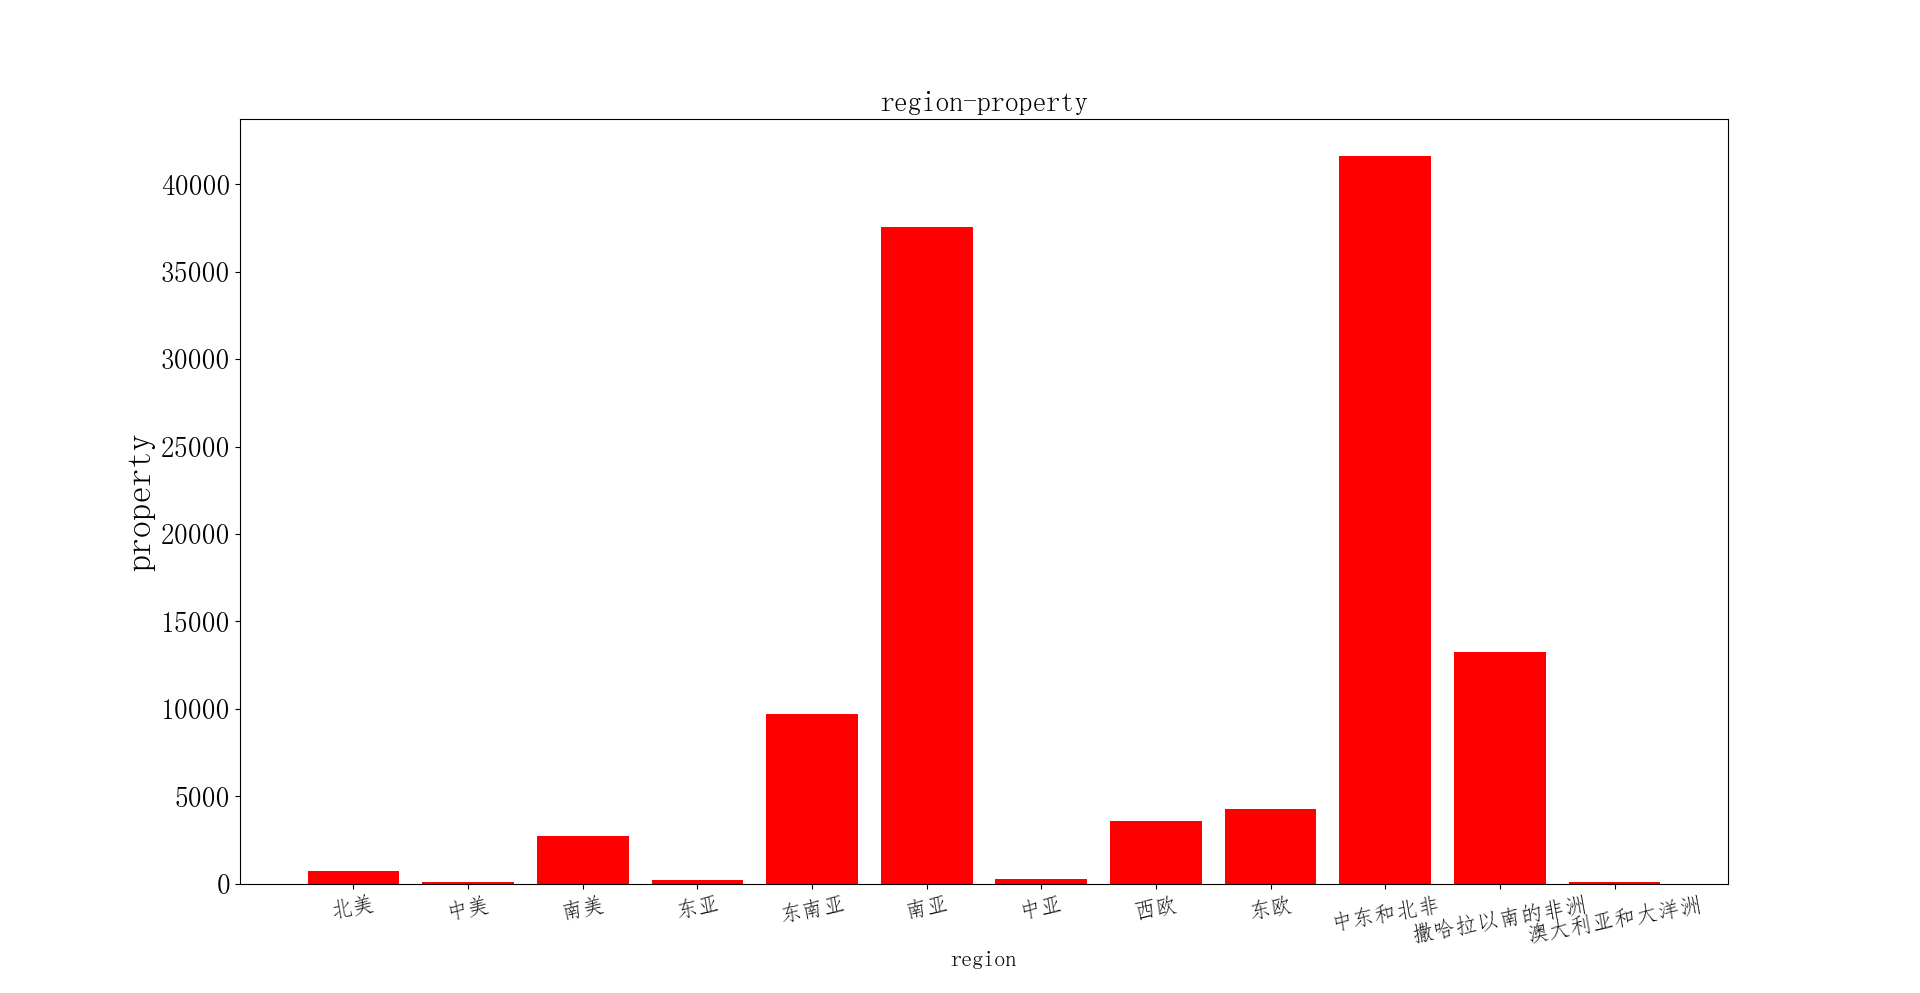
\includegraphics[width=.5\textwidth]{figures//img//Figure_1-15.png}
    }
    \caption{袭击事件发生次数、死亡人数、受伤人数和财产损失按地区分布统计图}
    \label{tab:地区分布}
\end{figure}

图\ref{tab:地区分布}利用条形统计图对不同地区的袭击事件发生次数、
死亡人数、受伤人数和财产损失进行了统计。
可以很直观的看到,中东和北非是恐怖袭击事件的多发地。
其次就是南亚地区,
其中撒哈拉以南的非洲和东南亚恐怖袭击事件发生次数也比其他地方要高。

\begin{figure}[htbp]
    \subfigure{
        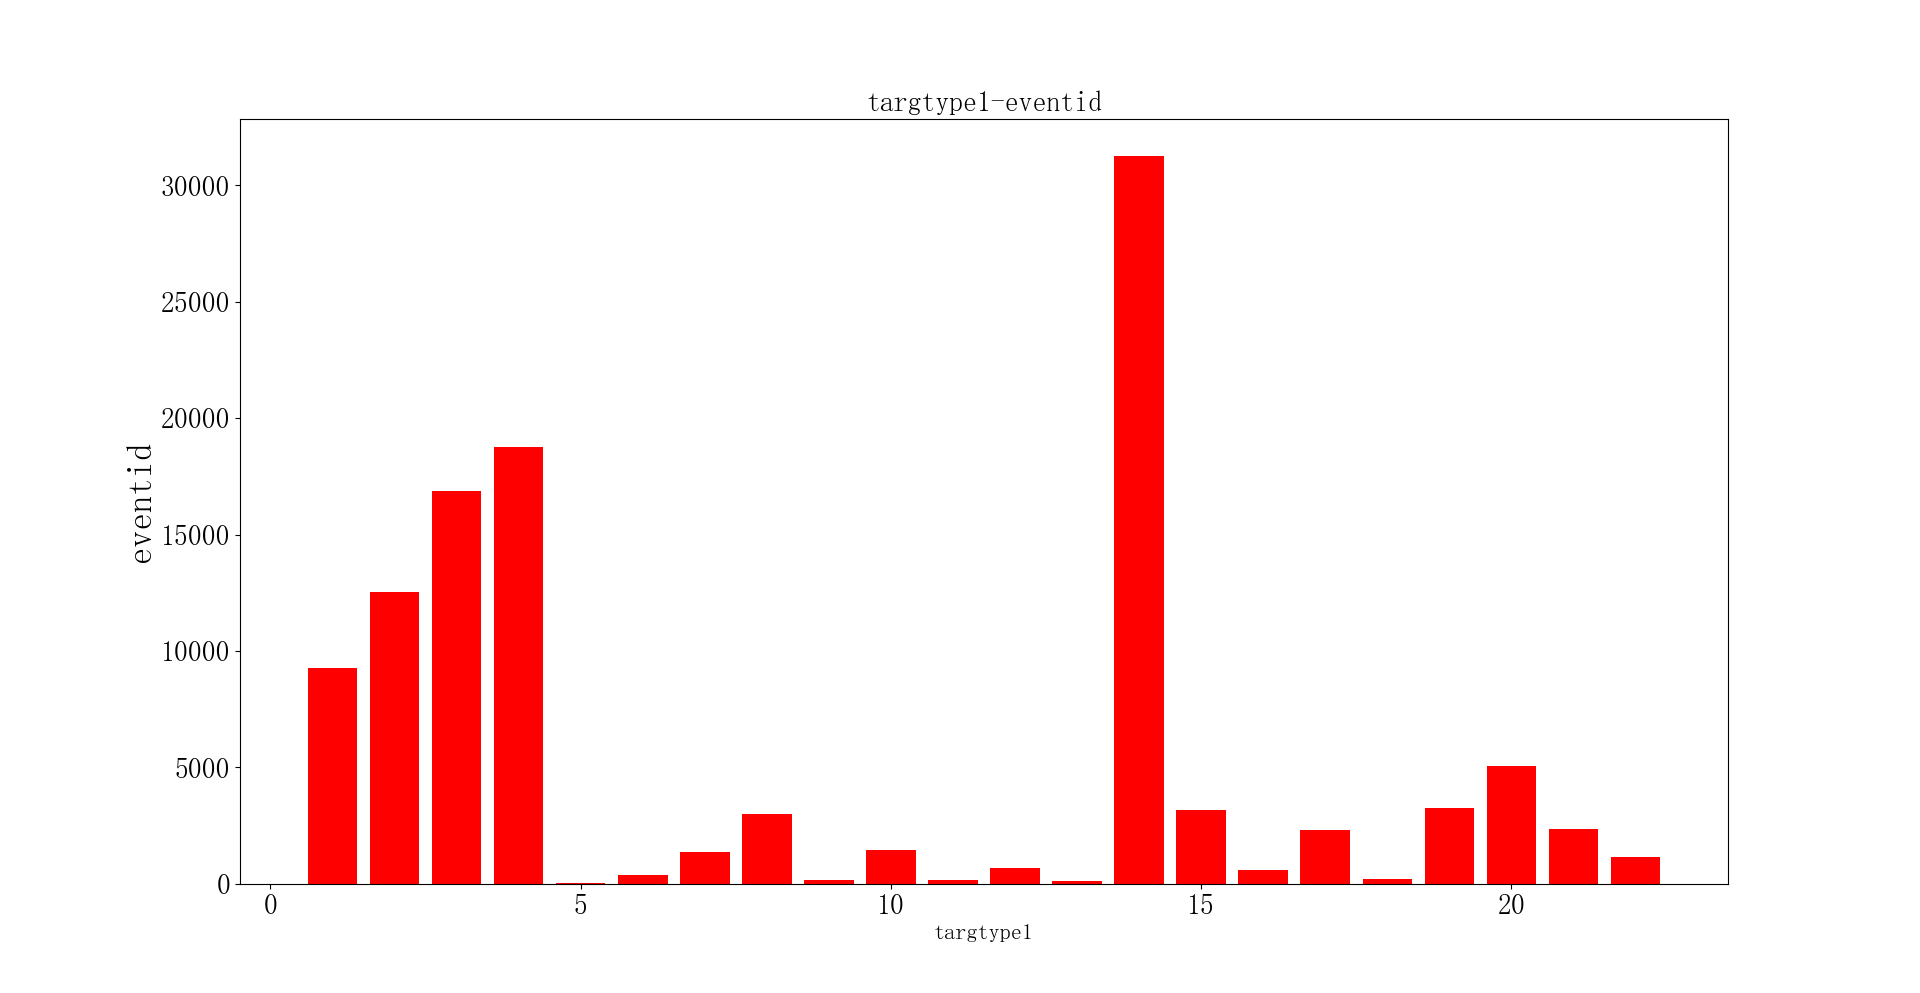
\includegraphics[width=.5\textwidth]{figures//img//Figure_1-16.png}

    }
    \subfigure{
        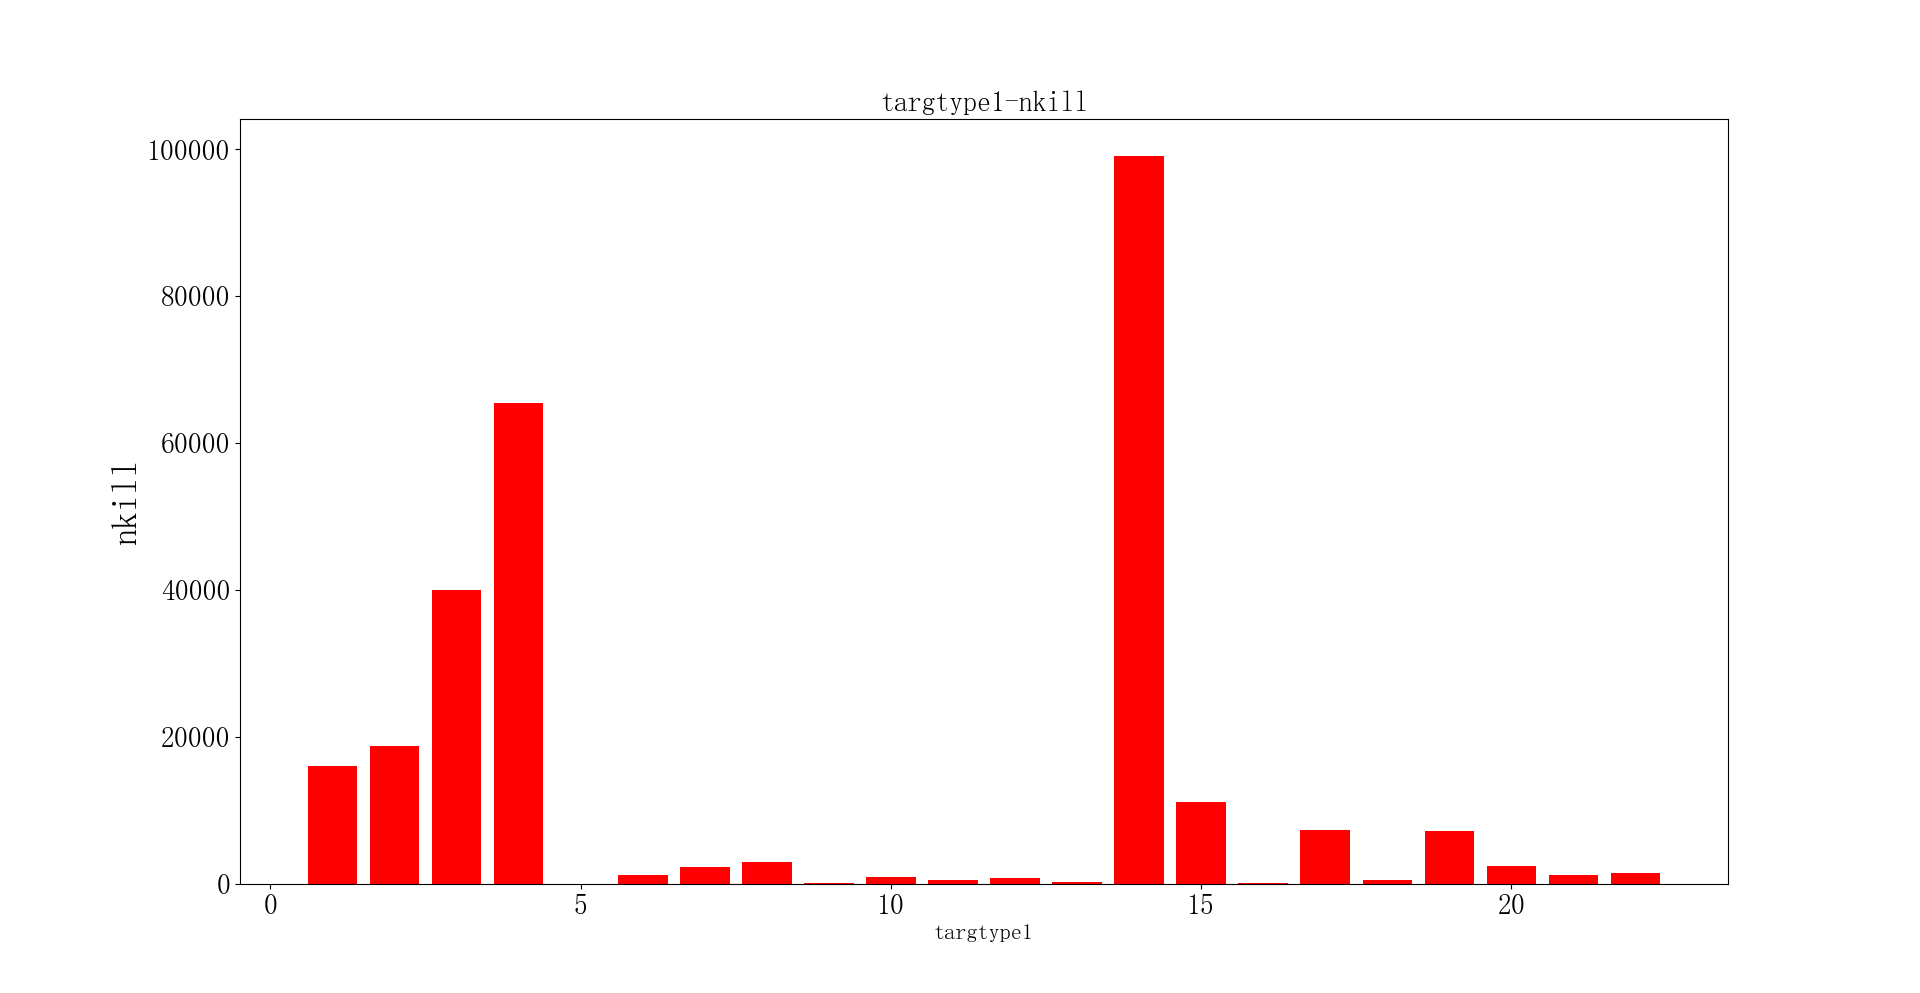
\includegraphics[width=.5\textwidth]{figures//img//Figure_1-17.png}
    }
    \subfigure{
        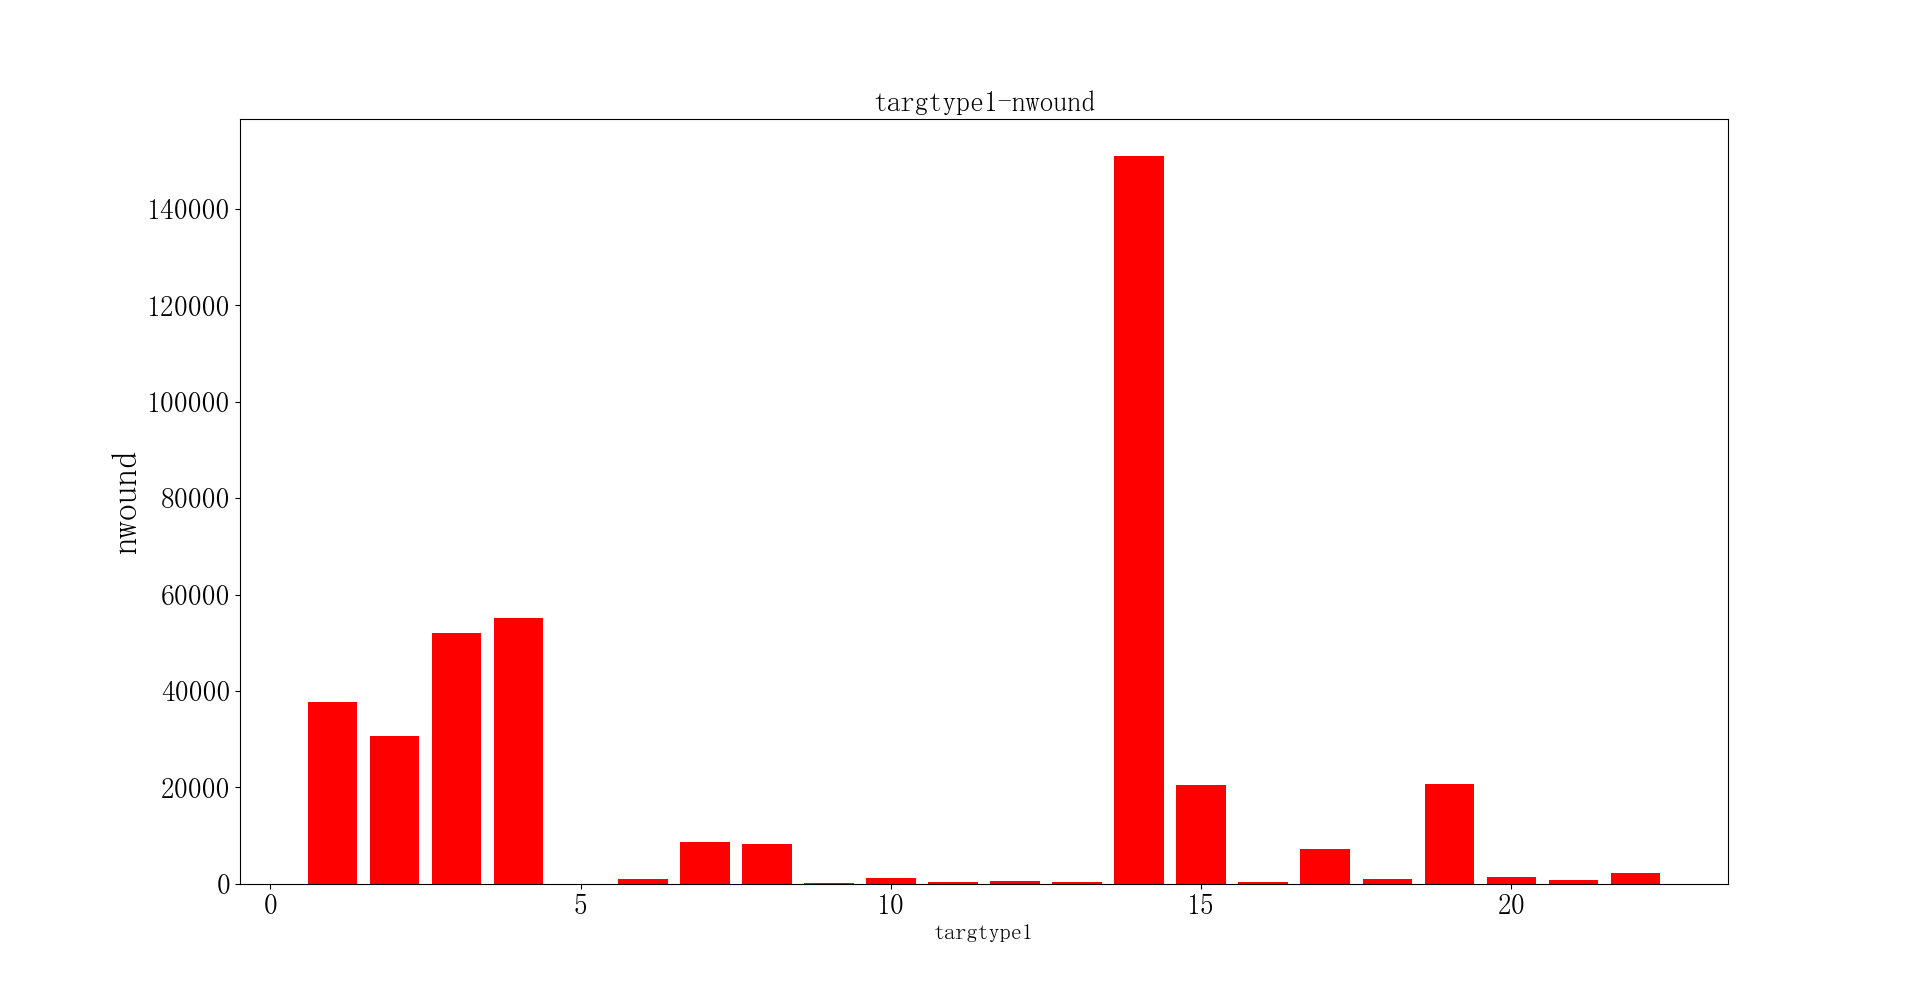
\includegraphics[width=.5\textwidth]{figures//img//Figure_1-18.png}
    }
    \subfigure{
        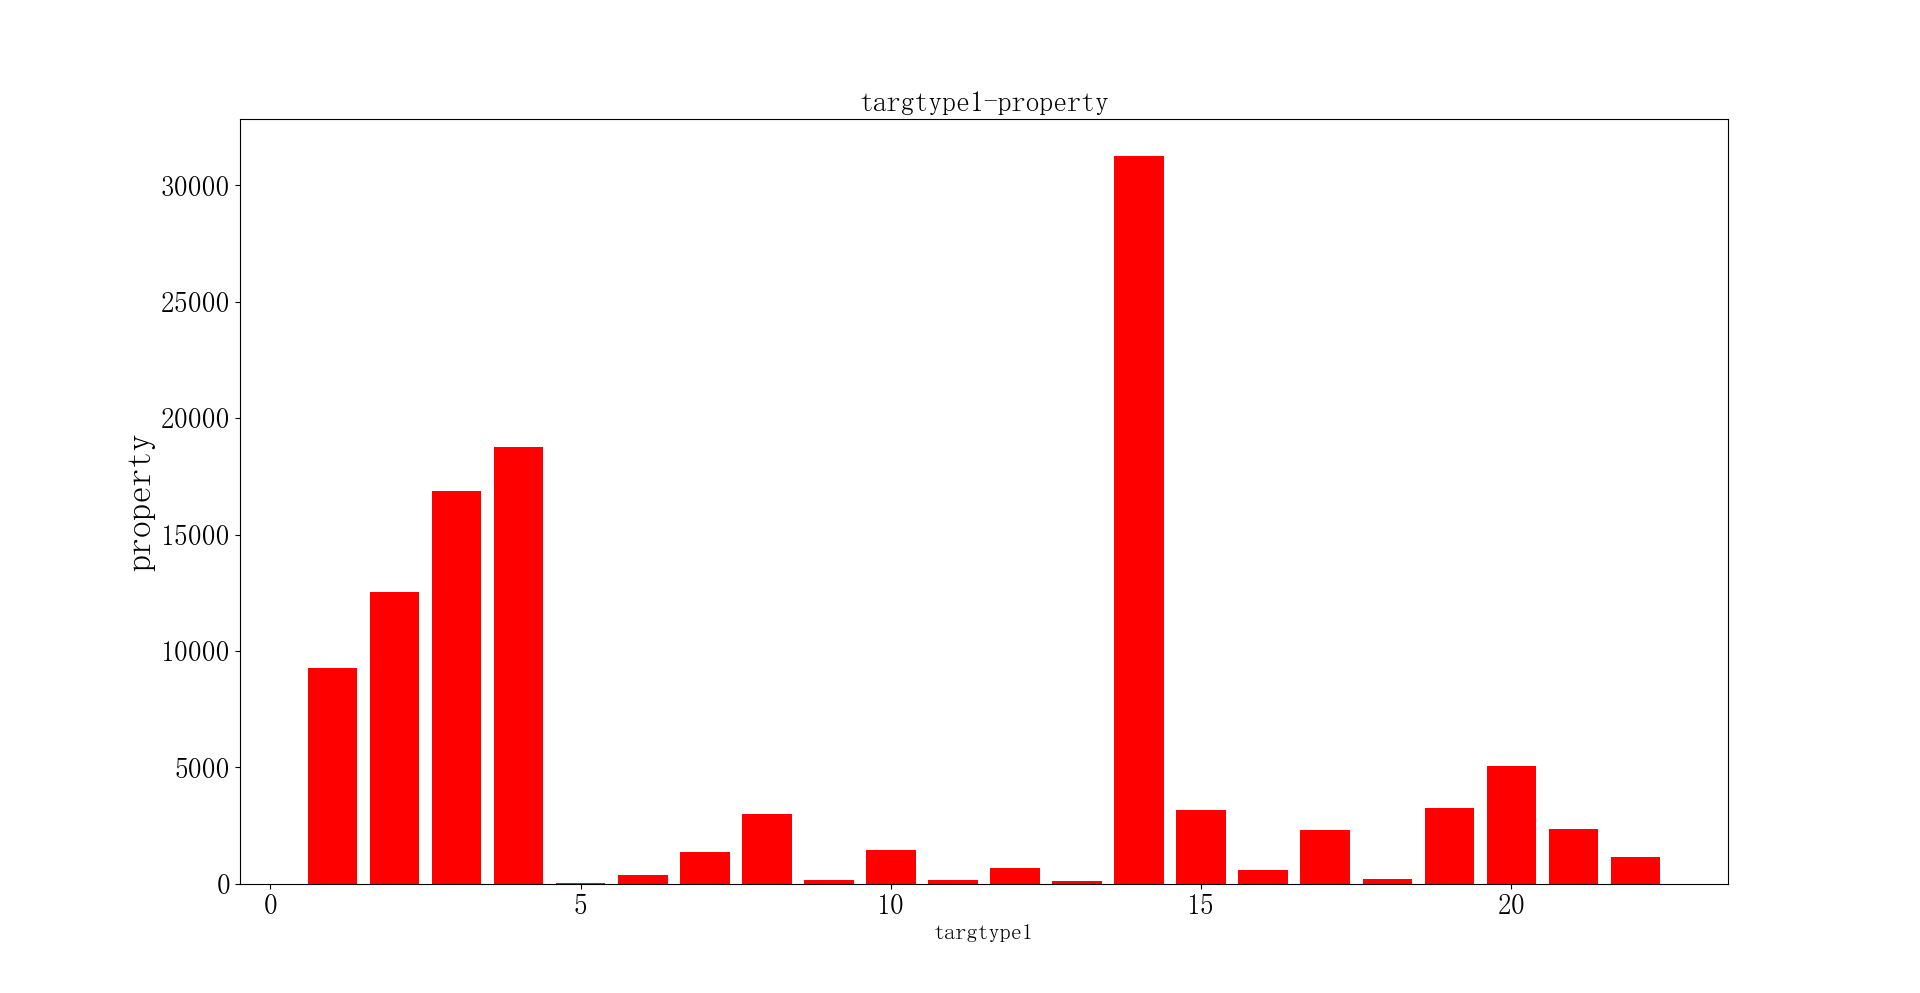
\includegraphics[width=.5\textwidth]{figures//img//Figure_1-19.png}
    }
    \caption{袭击事件发生次数、死亡人数、受伤人数和财产损失按地区分布统计图}
    \label{tab:袭击目标分布}
\end{figure}

图\ref{tab:袭击目标分布}利用条形统计图对不同目标/受害者类型的袭击目标被袭击的次数、
死亡人数、受伤人数以及财产损失进行了统计。
可以看到,其中14=公民自身和私有财产非常多。
1=商业、2 =政府(一般意义)、3 =警察、4 = 军事也占有比较大的比重。


\cite{李国辉2014全球恐怖袭击时空演变及风险分析研究}
中提到政治、经济、宗教或社会目标,
意图胁迫、恐吓或煽动更多的群众,
超出国际人道主义法律范围也是影响恐怖事件发生的原因。
恐怖袭击为:
由非国家的行动者为了获取一定的政治、
经济、宗教或社会目的通过威胁、
强迫或恐吓手段而实施的一种威胁或违法的暴力事件。
所以可以看到恐怖主义是与政治、经济、宗教等内容有关的。
因此,我们给出相关的统计图。

\begin{figure}[htbp]
    \subfigure{
        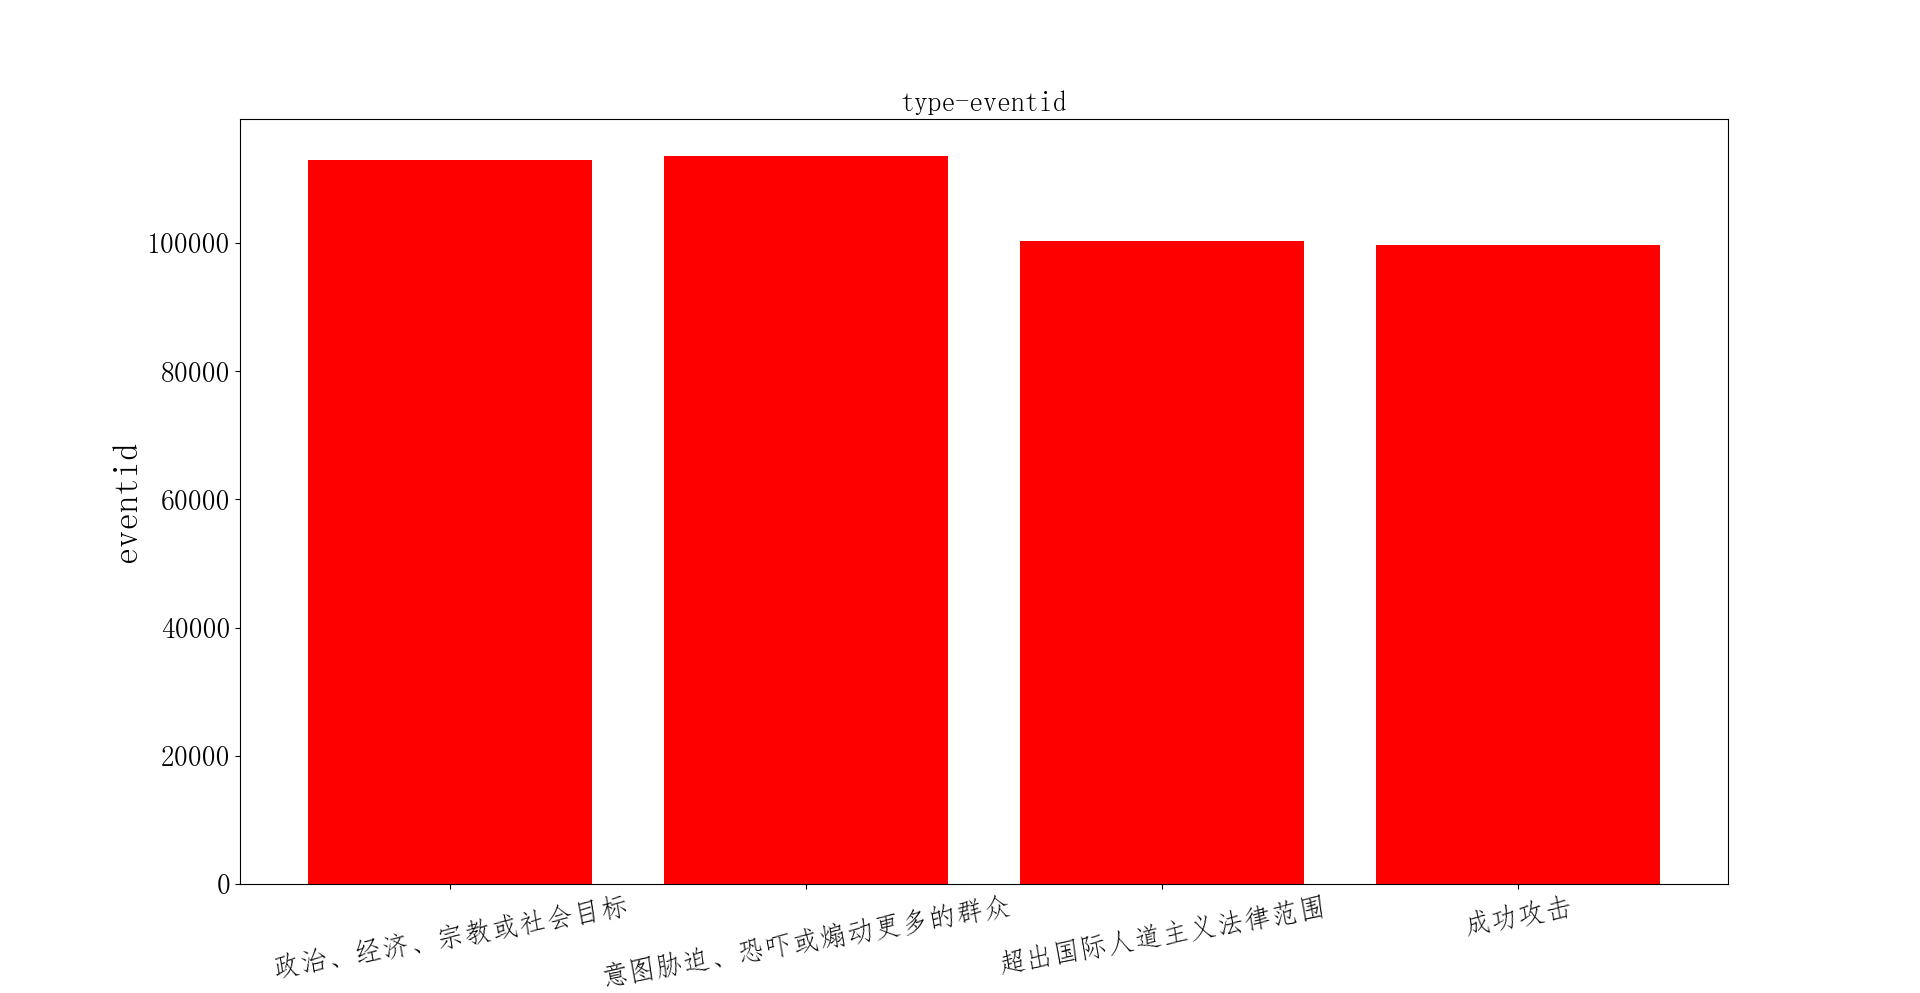
\includegraphics[width=.5\textwidth]{figures//img//Figure_1-20.png}

    }
    \subfigure{
        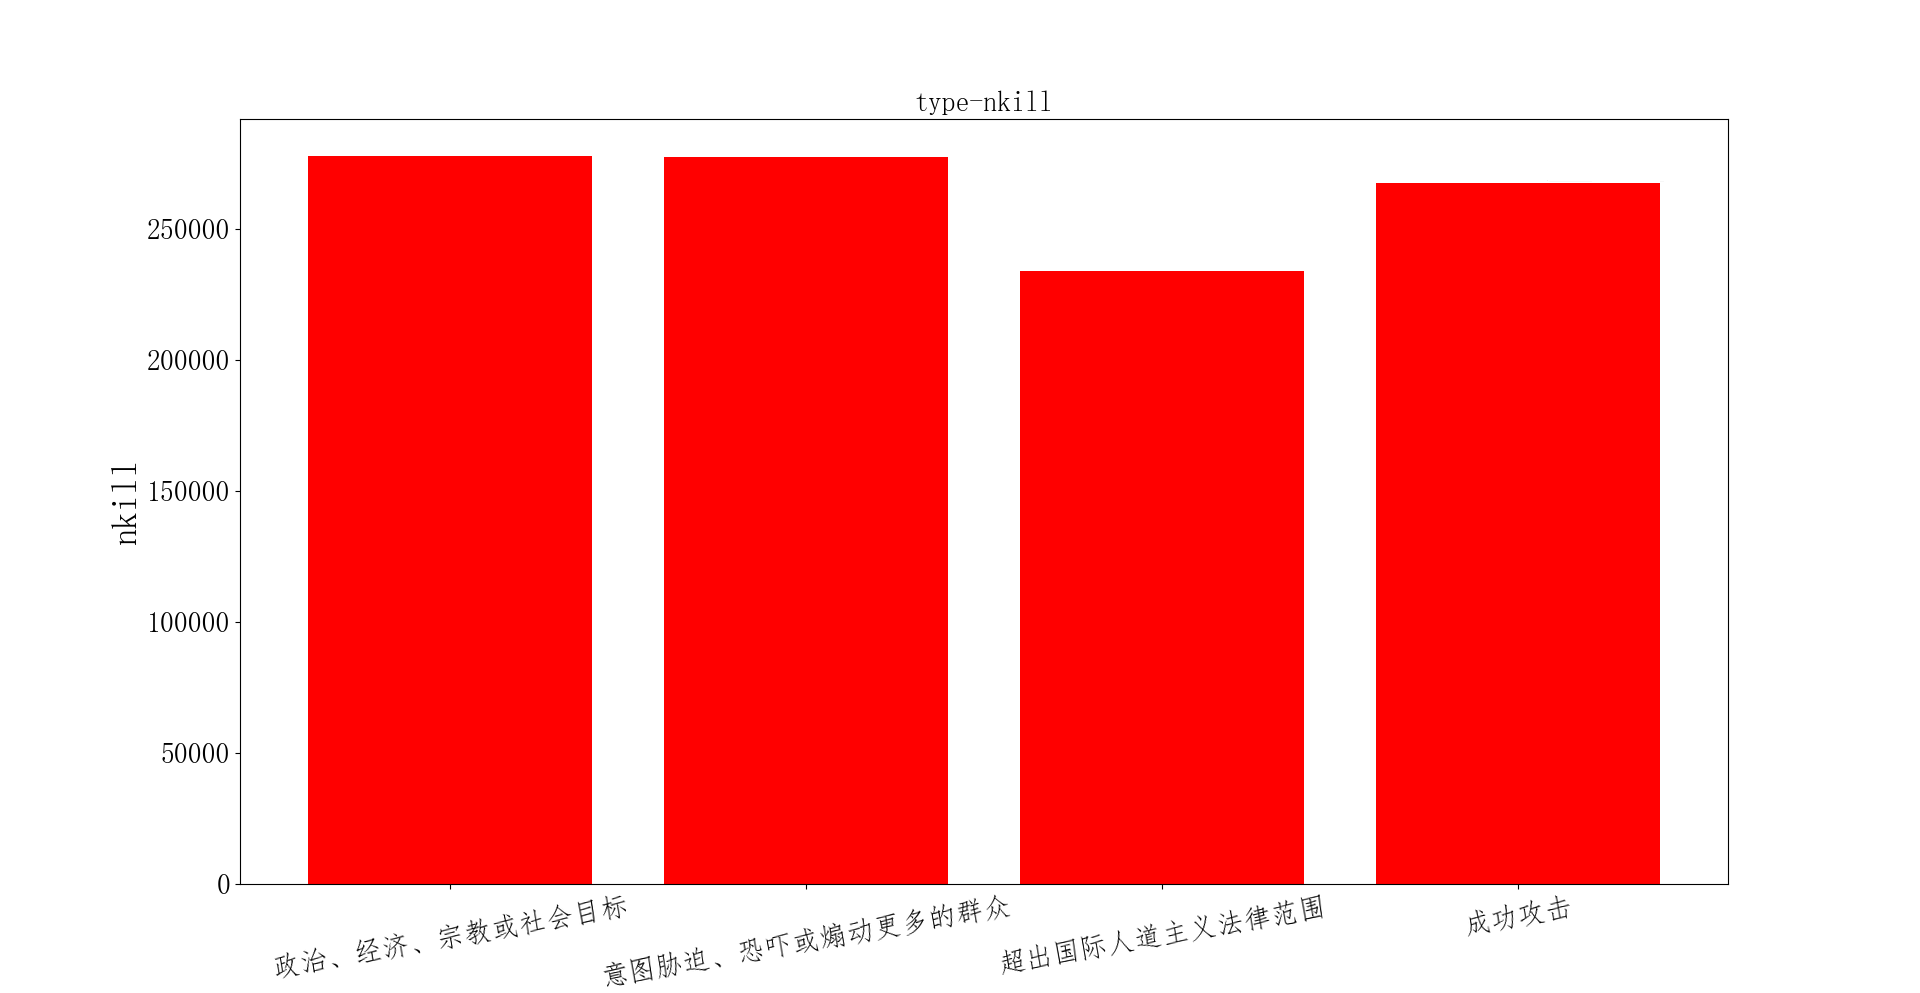
\includegraphics[width=.5\textwidth]{figures//img//Figure_1-21.png}
    }
    \subfigure{
        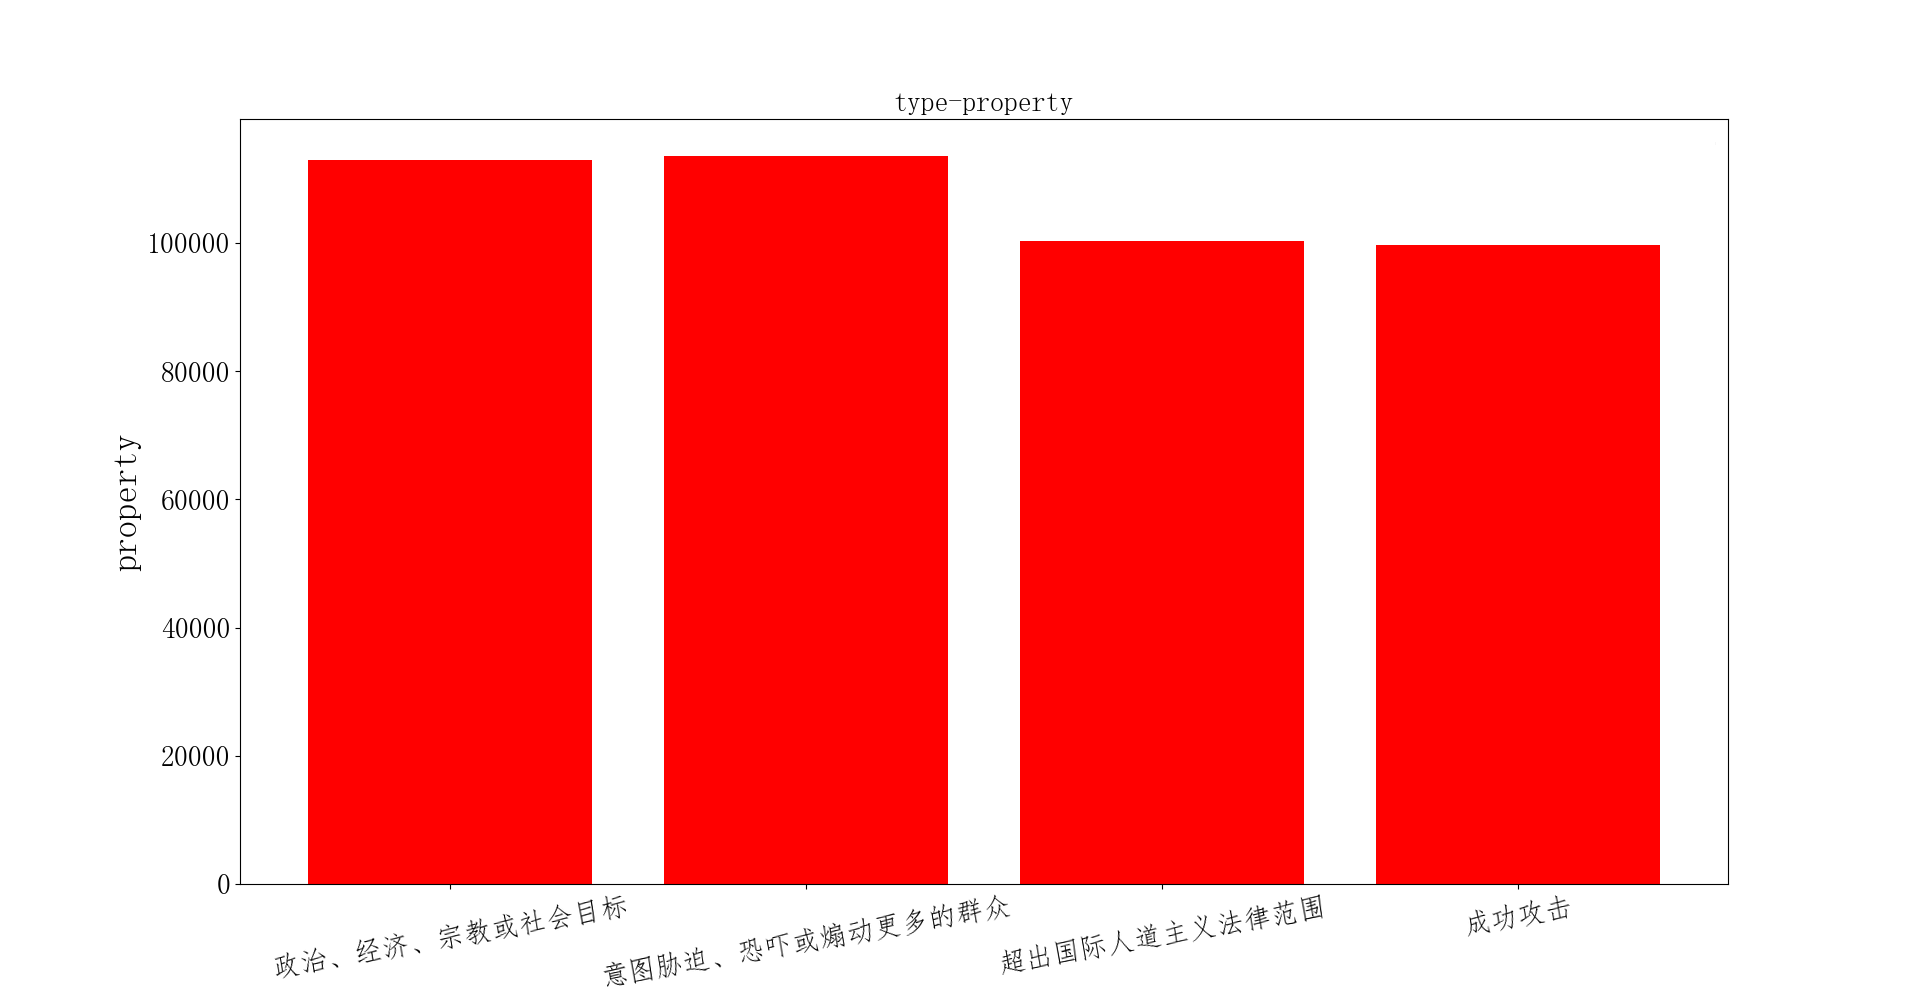
\includegraphics[width=.5\textwidth]{figures//img//Figure_1-22.png}
    }
    \subfigure{
        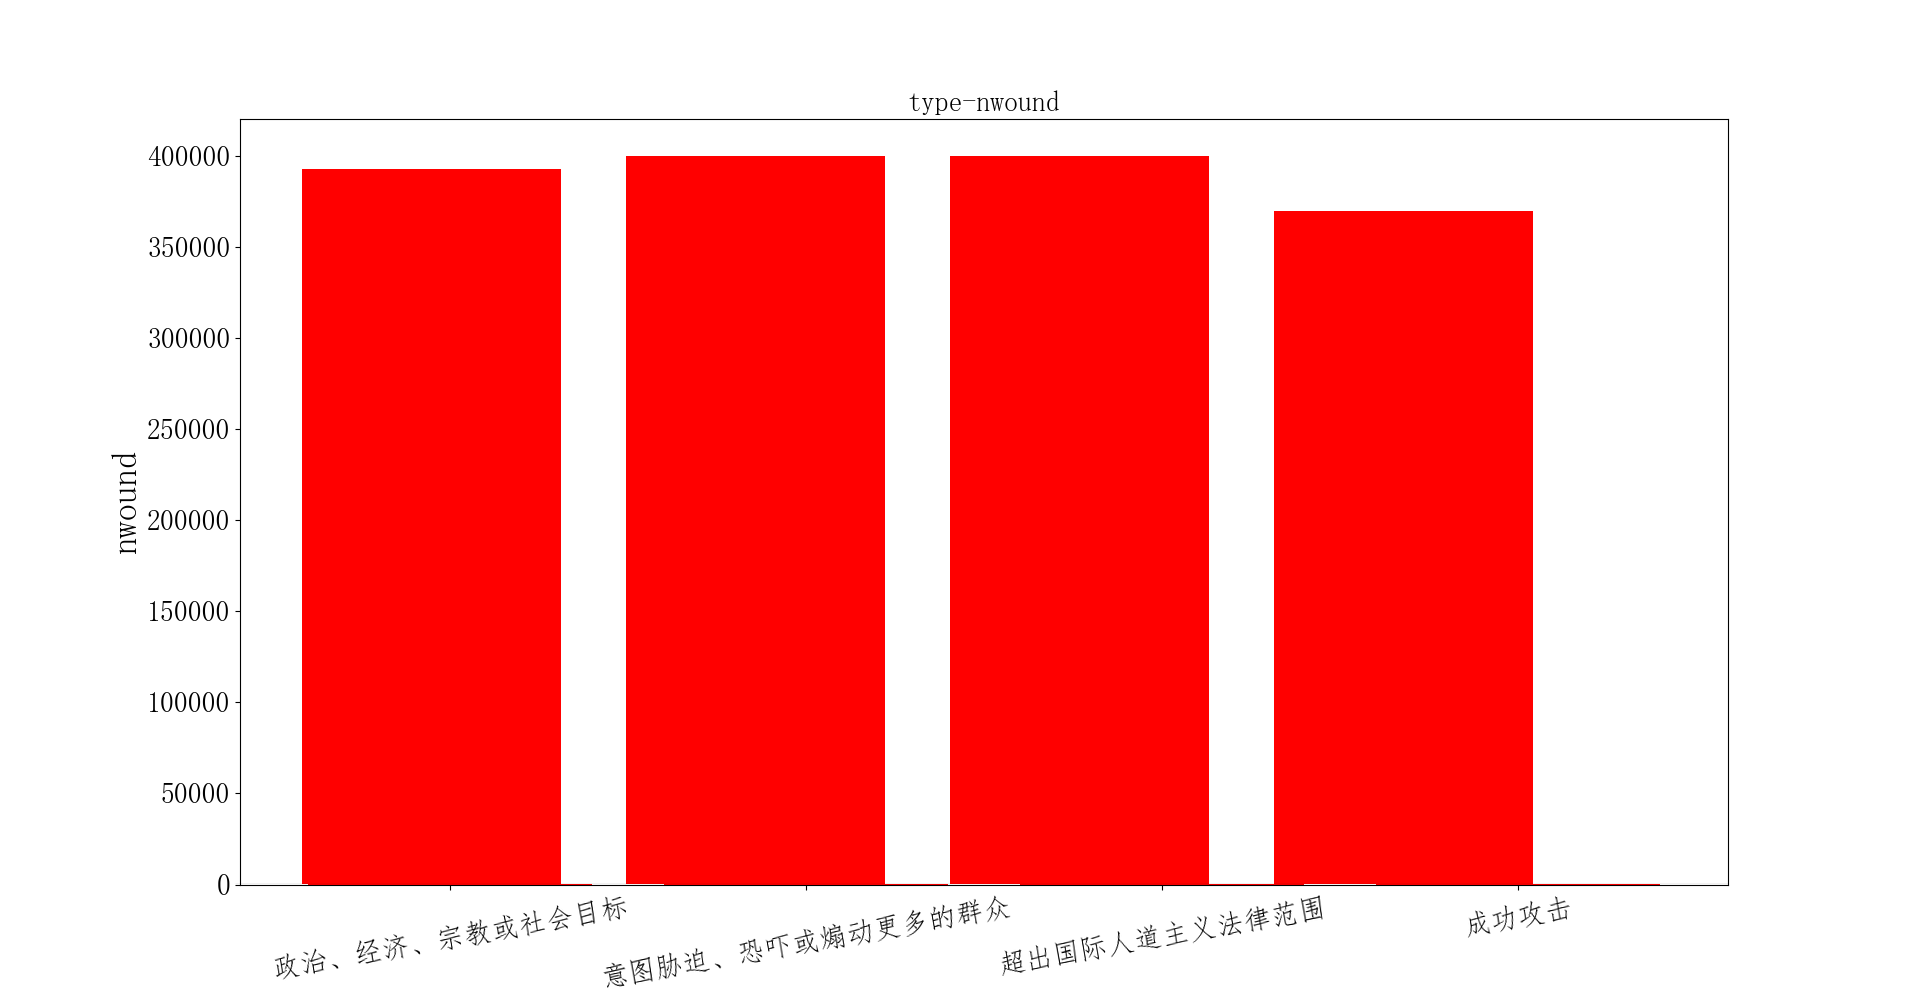
\includegraphics[width=.5\textwidth]{figures//img//Figure_1-27.png}
    }
    \caption{袭击事件发生次数、死亡人数、受伤人数和财产损失按入选标准统计图}
    \label{tab:入选标准分布}
\end{figure}

图\ref{tab:入选标准分布}利用条形统计图对恐怖袭击事件入选标准针对
袭击事件发生次数,死亡人数,受伤人数和财产损失进行了统计。
可以看到不同的类型都会由各种各样的恐怖袭击事件发生。
那么,通过这一统计,可以发现政治、经济、宗教或社会目标,
意图胁迫、恐吓或煽动更多群众这些都是造成恐怖袭击事件的原因。
所有,一个良好的教育和社会环境对于恐怖袭击事件得以控制也有着至关重要的作用。

\begin{figure}[htbp]
    \subfigure{
        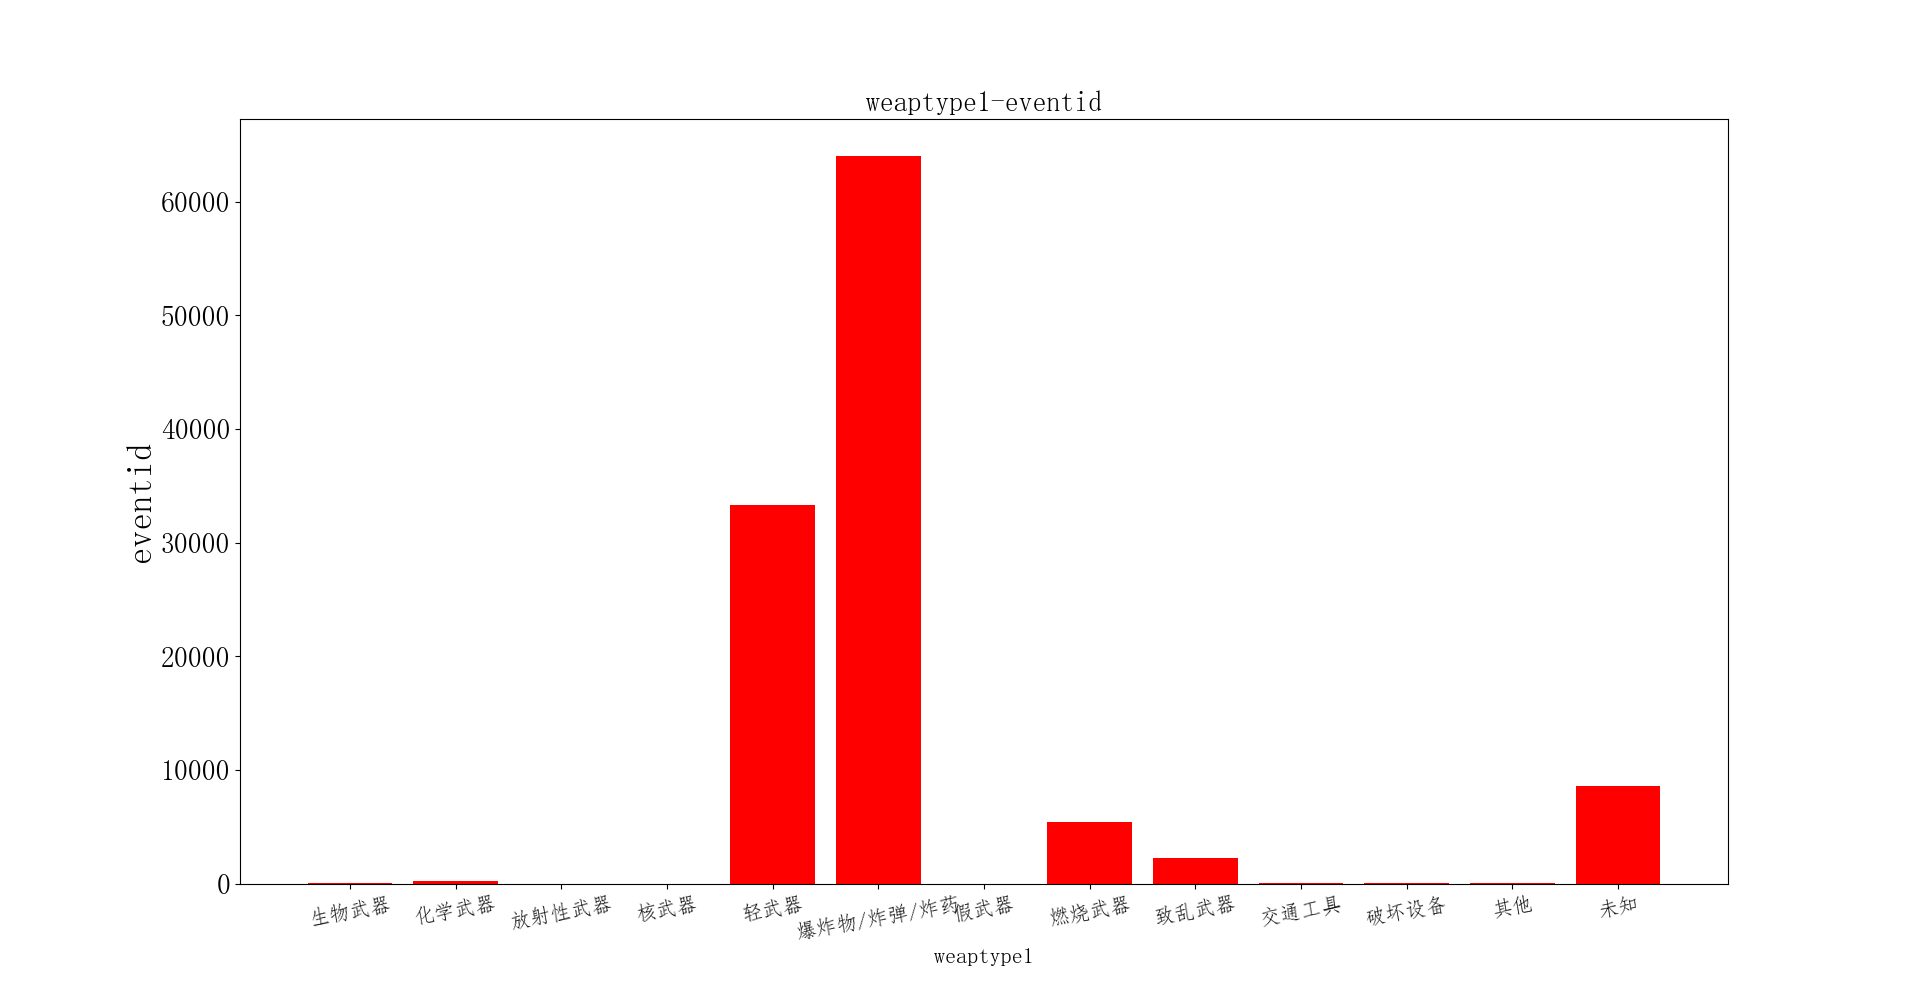
\includegraphics[width=.5\textwidth]{figures//img//Figure_1-23.png}

    }
    \subfigure{
        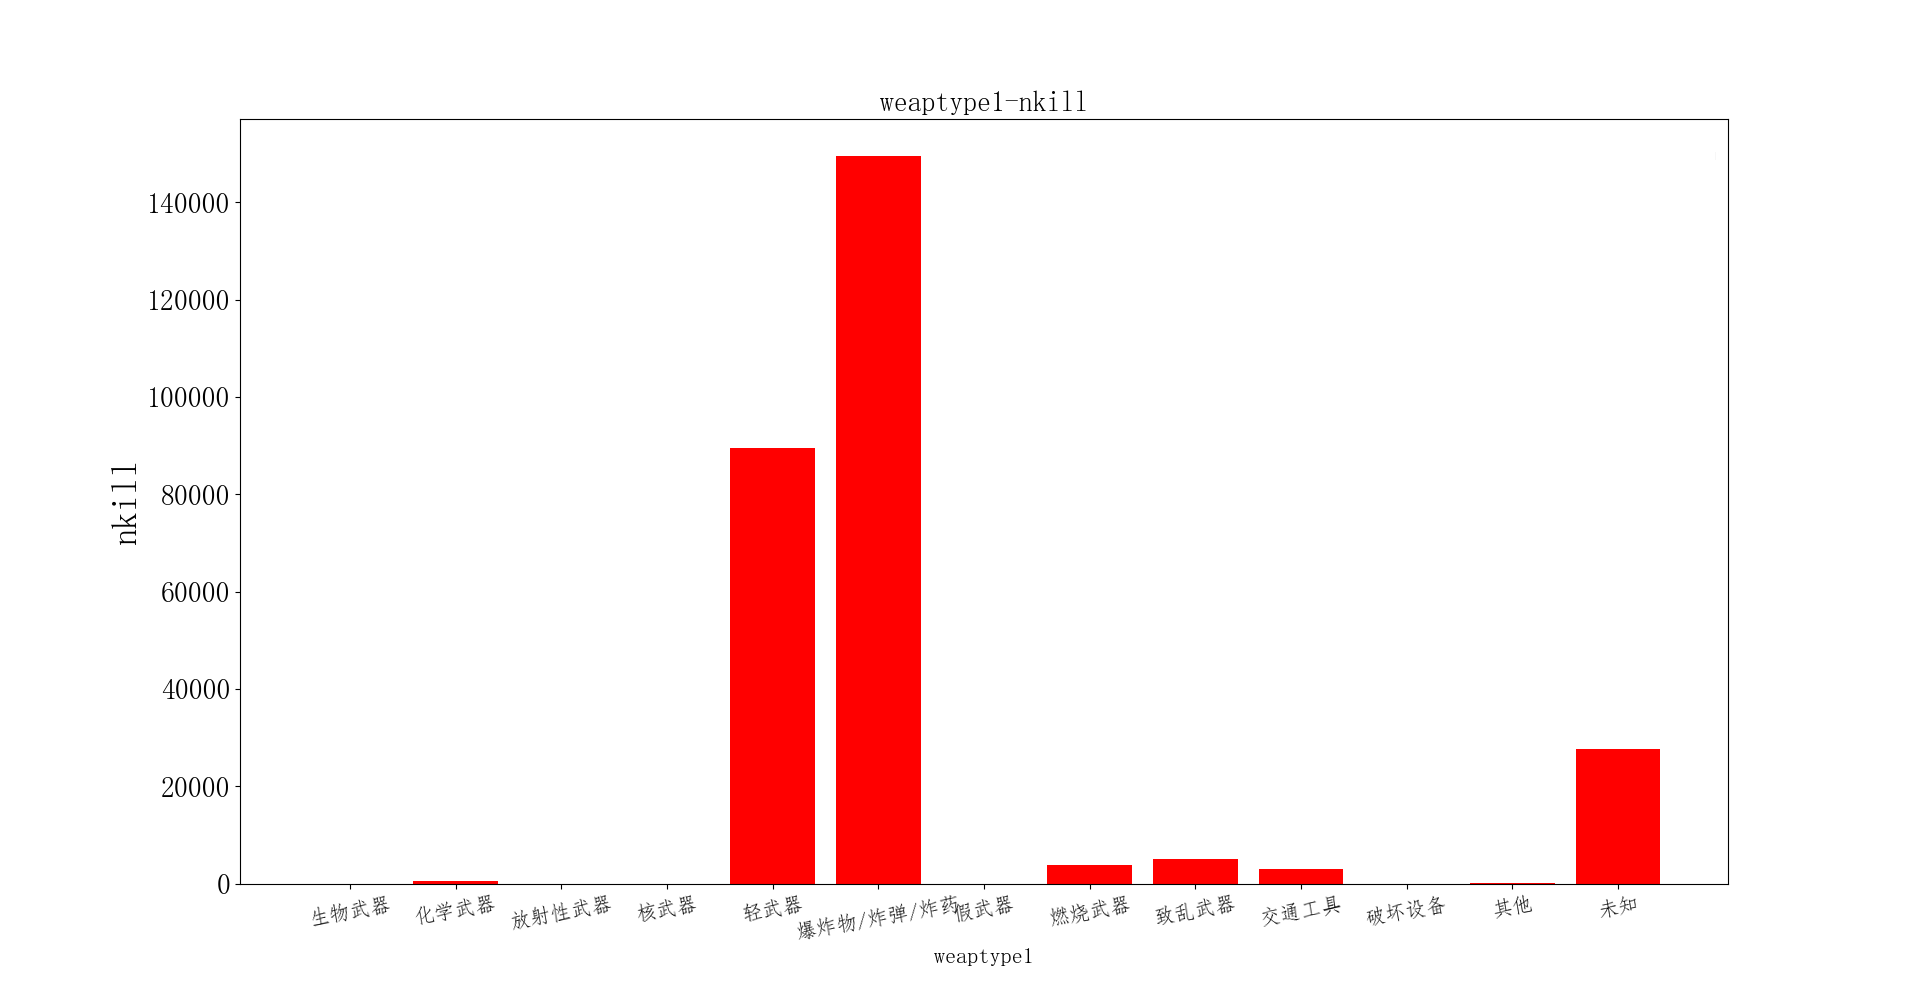
\includegraphics[width=.5\textwidth]{figures//img//Figure_1-24.png}
    }
    \subfigure{
        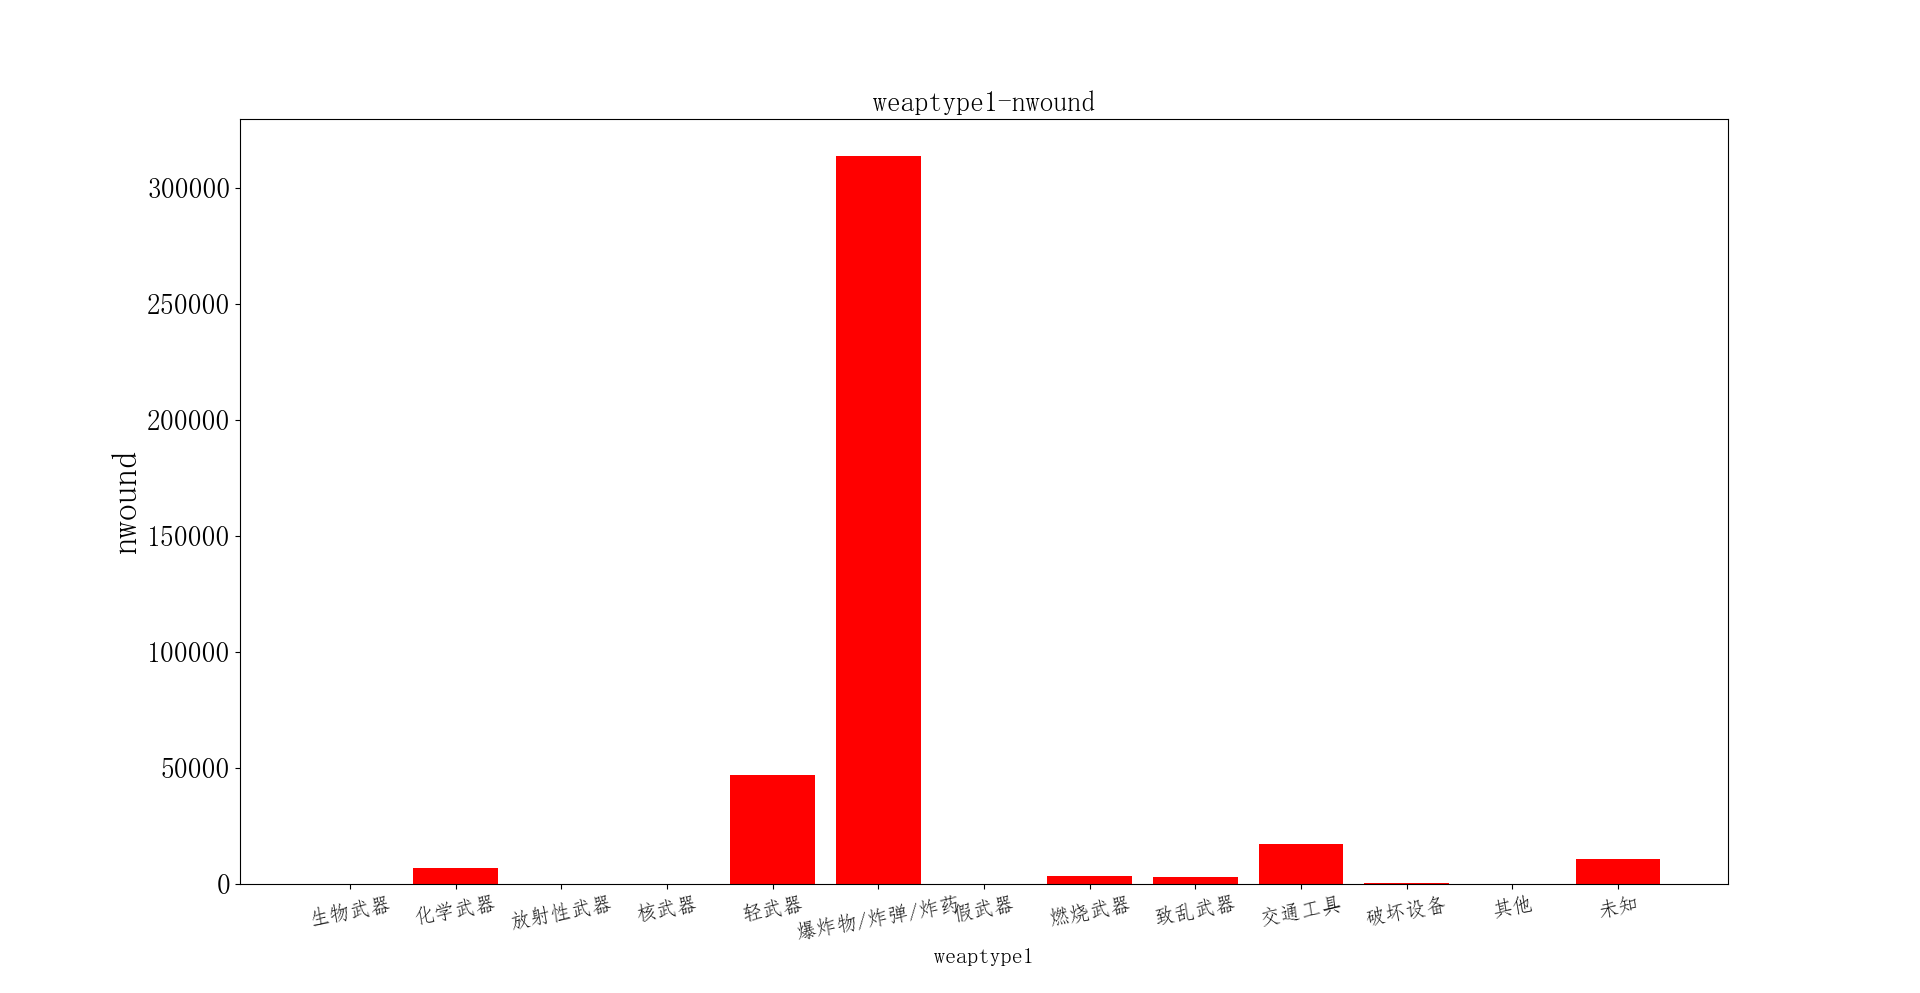
\includegraphics[width=.5\textwidth]{figures//img//Figure_1-25.png}
    }
    \subfigure{
        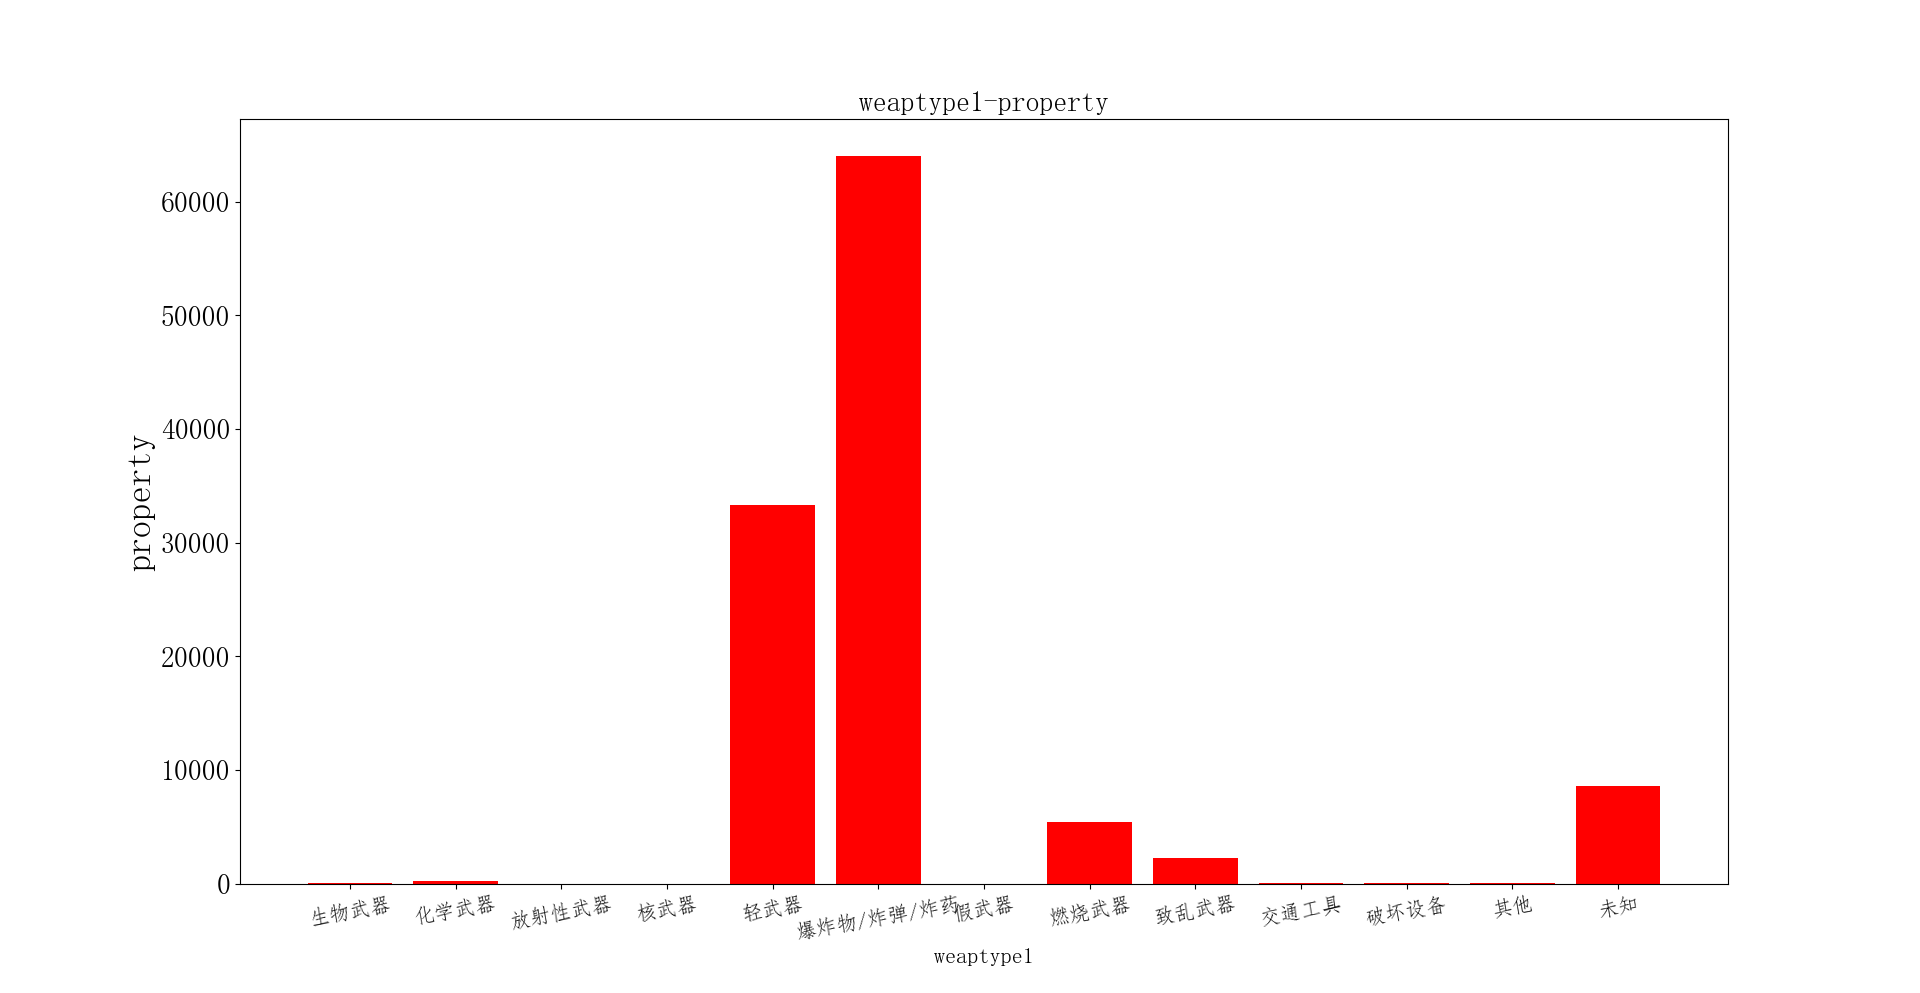
\includegraphics[width=.5\textwidth]{figures//img//Figure_1-26.png}
    }
    \caption{袭击事件发生次数、死亡人数、受伤人数和财产损失的攻击类型统计图}
    \label{tab:攻击类型分布}
\end{figure}

图\ref{tab:攻击类型分布}利用条形统计图,
对恐怖袭击事件的攻击类型进行了统计,可以发现,
大多数的恐怖袭击都是以爆炸物/炸弹/炸药和轻武器来实施的。
那么通过这一发现,那么我们是不是就可以建议国家可以
通过管制爆炸物炸药和轻武器来使得恐怖袭击事件得到控制。


\subsection{任务一}

\subsubsection{任务一分析}

针对任务一,
其中,
恐怖袭击事件的危害性不仅仅取决于人员伤亡和经济损失两方面,
\cite{贺怀清2012恐怖袭击事件不确定性度量及可视分析}
中将时间、地域性、袭击方式和针对目标作为恐怖袭击事件的危害性度量标准。
其中包含变量年(iyear)、
月(imonth)、
日(iday)、
国家(country)、
地区(region)、
攻击类型(attacktype)、
袭击目标(targtype1)、
袭击目标和国籍(natlty)、
武器类型(weaptype)、
伤亡人数(nkill)。
\cite{李国辉2014全球恐怖袭击时空演变及风险分析研究}
中讲到将恐怖袭击的影响因素分为直接影响和间接影响,
其中直接影响包括人员伤亡和经济损失,
这些和恐怖分子采用的武器类型、袭击方式和袭击目标是紧密相关的。
间接影响包括对社会秩序的影响,
这可能是与社会民主制度、政治参与度等有关。
同时,恐怖袭击还与地理空间属性有关。
通过对上面两篇文章的阅读,以及对GTD数据的解析,
通过查阅灾害事件危害等级相关资料,
我们发现除了上述提到的度量标准,
事件是否持续,
财产损失,
以及是否是成功的袭击也是影响恐怖事件危害级别的影响因素。
所以这里我们在对相关文献以及相关资料中的危害影响因素进行了总结。
最后我们挑选了19个变量进行高斯混合聚类分析,
并通过Shanno熵来计算权重。
最终得到危害级别。

\subsubsection{任务一求解}

针对任务一,我们主要做了如下工作:
\begin{itemize}
  \item 搜集资料查找影响恐怖事件危害级别的因素。
  \item 整理好数据集进行高斯混合聚类。
  \item 利用Shanno熵计算变量权值。
  \item 将聚类结果和权值结合计算危害级别。
\end{itemize}

通过\cite{贺怀清2012恐怖袭击事件不确定性度量及可视分析}
和\cite{李国辉2014全球恐怖袭击时空演变及风险分析研究}
我们确定了如下影响因素:
年(iyear)、
月(imonth)、
日(iday)、
国家(country)、
地区(region)、
攻击类型(attacktype)、
袭击目标(targtype1)、
袭击目标和国籍(natlty)、
武器类型(weaptype)、
伤亡人数(nkill)、
凶手受伤人数(nwoundte)、
事件是否持续(extened)、
财产损失(property)、
纬度(latitude)、
经度(longitude)、
成功的攻击(success)、
目标/受害者类型(targtype1)、
目标/受害者的国籍(natlty1)、
标准1:政治、经济、宗教或社会目标(crit1)、
标准2:意图胁迫、恐吓或煽动更多的群众(crit2)、
标准3:超出国际人道主义法律范围(crit3)、

熵:表示随机变量不确定性,即混乱程度的量化指标。
香农熵的计算公式:
\begin{equation}
 H(X) = - \sum_{x} P(X)log_2 [P(x)]
 \label{tab:Shanno}
\end{equation}

\begin{table}
\centering
\caption{Shanno 熵结果}
\begin{tabular}{|c|c|c|c|}
  \hline
          1          &              2       &         3           &           4   \\
  \hline
   0.301653642592234 &  0.02624256028349834 & 0.08659082720203944 & 0.1668626935643827 \\
  \hline
\end{tabular}
\end{table}

高斯混合模型(Gaussian Mixture Model ,GMM)也是原型聚类,
该模型不需要先验知识,可以实现模型结构和参数的自动学习,
而且因为该分布由k个混合部分组成,所以它本身可以任意复杂,
通过增加model 的数量(即聚类的k值),可以任意的逼近任何连续的概率分布。

高斯概率密度公式:
\begin{equation}
p(x) = \frac{1}{(2\pi)^(\frac{n}{2})
(| \sum |)^{\frac{1}{2}})} e^{-\frac{1}{2} (x-\mu)^T (\sum)^{-1}(x-\mu)}
\end{equation}

高斯混合分布为:
\begin{equation}
p(x) = \sum_{k=1}^K \alpha_i p(x|\mu_i,\sum i)
\end{equation}

\begin{table}
\centering
\caption{聚类之后的变量求和结果}
\begin{tabular}{|c|c|c|c|c|}
  \hline
   labels & eventid & nkill & nwound & property   \\
  \hline
     0    & 63026   & 100613& 182137 & 27630      \\
  \hline
     1    &  6565   & 26628 & 12171  & 2120       \\
  \hline
     2    & 18710   & 8718  & 0      & 7168       \\
  \hline
     3    &  19204  & 15744 & 17116  & 3981       \\
  \hline
     4    &  6678   & 127842& 190142 & 2873       \\
  \hline
\end{tabular}
\end{table}

我们利用每个变量的求和与其对应的权值进行相乘求和:
\begin{equation}
  Y = \lambda_1 x_1 + \lambda_2 x_2 + \lambda_3 x_3 + \lambda_4 x_4
\end{equation}

结果如下:

\begin{table}
\centering
\caption{分级结果}
\begin{tabular}{|c|c|c|c|c|}
  \hline
          1    &    2       &   3      &     4   &   5  \\
  \hline
    42034.17   &  22313.29  &  8352.48 &  7068.79 & 4086.79\\
  \hline
\end{tabular}
\end{table}

对上述聚类结果,
我们进行了统计,
绘制了饼图来反映每一个级别的事件在整个数据集中所占比例。

%\begin{center}
\begin{figure}[htbp]
\centering
  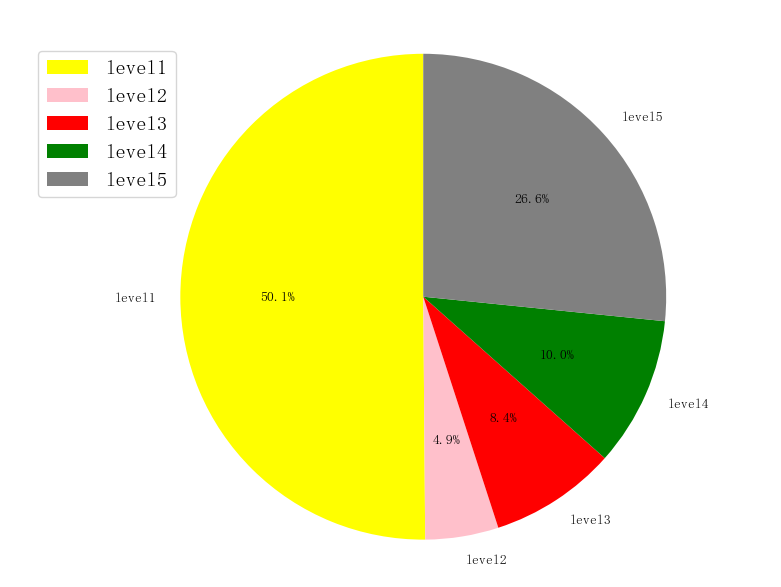
\includegraphics[width=.5\textwidth]{figures//img//Figure12.png}
  \caption{危害级别分布图}
  \label{tab:聚类结果}
\end{figure}
%\end{center}

图\ref{tab:聚类结果}可以看到危害级别为第一级所占比重为50.1\%,
危害级别为第二级所占比重为4.9\%,
危害级别为第三级所占比重为8.4\%,
危害级别为第四级所占比重为10\%,
危害级别为第五级所占比重为26.6\%。


\subsection{任务二}

\subsubsection{任务二分析}

题目要求针对2015、2016年度发生的、
尚未有组织或个人宣城负责的恐怖袭击事件,
来对案件进行分类,
最终按照组织或者个人的危害性大小排序。
我们考虑到最终需要预测得到2017年度恐怖分子关于典型事件的嫌疑度,
所以我们利用2015、2016和2017年度的数据进行分类。
对可能是同一恐怖组织或个人在不同时间、
不同地点多次作案的若干案件归为一类。
那么我们把不同的犯罪团伙进行了分类,
利用KNN算法计算未知案件到不同类之间的距离,
选择排名前五的犯罪嫌疑人/团伙。

\subsubsection{任务二求解}
首先我们利用XGBoost算法对未知样本进行预测,
我们用到了年(iyear)、
月(imonth)、
日(iday)、
国家(country)、
地区(region)、
攻击类型(attacktype)、
袭击目标(targtype1)、
袭击目标和国籍(natlty)、
武器类型(weaptype)、
伤亡人数(nkill)、
凶手受伤人数(nwoundte)、
事件是否持续(extened)、
财产损失(property)、
纬度(latitude)、
经度(longitude)、
成功的攻击(success)、
目标/受害者类型(targtype1)、
目标/受害者的国籍(natlty1)、
标准1:政治、经济、宗教或社会目标(crit1)、
标准2:意图胁迫、恐吓或煽动更多的群众(crit2)、
标准3:超出国际人道主义法律范围(crit3)、
进行训练,然后对未知属性进行预测。

\textbf{XGBoost}
是GB算法的高效实现,
XGBoost中的基学习器除了可以是CART(gbtree)也可以是线性分类器(gblinear)。
\begin{itemize}
  \item xgboost在目标函数中显示的加上了正则化项,
  基学习为CART时,
  正则化项与树的叶子节点的数量T和叶子节点的值有关。

  \begin{equation}
  L(\phi) = \sum_i l(\widehat{y}_i,y_i) + \sum_k \Omega(f_k)
  \end{equation}
  where
  \begin{equation}
  \Omega(f) = \gamma T + \frac{1}{2} \lambda \| w \|^2
  \end{equation}

  \item GB中使用Loss Function对f(x)的一阶导数计算出伪残差用于学习生成fm(x),
  xgboost不仅使用到了一阶导数,还使用二阶导数。\\
  第t次的loss:
  \begin{equation}
  L^(t) = \sum_{i+1}^n l(y_i,\widehat{y}_i^{(t-1)}+f_t (X_i)) + \Omega(f_t)
  \end{equation}

  \item 上面提到CART回归树中寻找最佳分割点的衡量标准是最小化均方差,
  xgboost寻找分割点的标准是最大化,lamda,gama与正则化项相关。
  \begin{equation}
  L_split = \frac{1}{2}
  [ \frac{(\sum_{i\in{I_L}} g_i)^2}{\sum_{i\in{I_L}} h_i +\lambda}
  + \frac{(\sum_{i\in{I_R}} g_i)^2}{\sum_{i\in{I_R}} h_i +\lambda}
  - \frac{\sum_{i\in{I}} g_i)^2}{\sum_{i\in{I}} h_i +\lambda} ] - \gamma
  \end{equation}
\end{itemize}

表\ref{tab:xgboost预测结果}
为我们利用XGBoost模型对未知组织/个人的犯罪案件进行预测得到的结果。

\begin{table}
\centering
\caption{XGBoost预测结果}
\begin{tabular}{|c|c|}
  \hline
  % after \\: \hline or \cline{col1-col2} \cline{col3-col4} ...
  事件编号 & 犯罪嫌疑人 \\
  \hline
  201701090031 & Islamic State of Iraq and the Levant (ISIL)  \\
  \hline
  201702210037 & Islamic State of Iraq and the Levant (ISIL) \\
  \hline
  201703120023 & Boko Haram \\
  \hline
  201705050009 & Taliban \\
  \hline
  201705050010 & Taliban \\
  \hline
  201707010028 & Maoists  \\
  \hline
  201707020006 & Islamic State of Iraq and the Levant (ISIL)  \\
  \hline
  201708110018 & Taliban  \\
  \hline
  201711010006 & Taliban  \\
  \hline
  201712010003 &  Islamic State of Iraq and the Levant (ISIL)  \\
  \hline
\end{tabular}
\label{tab:xgboost预测结果}
\end{table}

\textbf{KNN}
通过测量不同特征值之间的距离进行分类。
如果一个样本在特征空间中的k个最相似
(即特征空间中最邻近)的样本中的大多数属于某一个类别,
则该样本也属于这个类别。
KNN算法中,所选择的邻居都是已经正确分类的对象。
该方法在定类决策上只依据最邻近的一个
或者几个样本的类别来决定待分样本所属的类别。
这里通过\ref{tab:欧氏距离}欧氏距离来计算近邻对象:

\begin{equation}
  d(x,y) = \sqrt{\sum_{k=1}^n (x_k - y_k)^2}
  \label{tab:欧氏距离}
\end{equation}

我们利用KNN模型思想来进行该问题的建模。
首先将同一样本标签(犯罪团伙/个人)的数据作为训练集,
未知样本标签的数据作为训练集,
来训练得到未知样本标签可能的犯罪嫌疑人。


\begin{table}
\centering
\caption{KNN算法分类结果}
\resizebox{\textwidth}{35mm}{
\begin{tabular}{|c|c|c|c|c|c|}
  \hline
  % after \\: \hline or \cline{col1-col2} \cline{col3-col4} ...
  事件编号
  & 1号嫌疑人
  & 2号嫌疑人
  & 3号嫌疑人
  & 4号嫌疑人
  & 5号嫌疑人
  \\
  \hline
  201701090031
  & Islamic State of Iraq and the Levant (ISIL)
  & Al-Qaida in the Arabian Peninsula (AQAP)
  & Abu Sayyaf Group (ASG)
  & Abdul Ghani Kikli Militia
  & Abu Amarah Battalion
  \\
  \hline
  201702210037
  & Islamic State of Iraq and the Levant (ISIL)
  & Abu Sayyaf Group (ASG)
  & Abbala extremists
  & Abu Sayyaf Group (ASG)
  & Abdul Ghani Kikli Militia
  \\
  \hline
  201703120023
  & Boko Haram
  & Abu Sayyaf Group (ASG)
  & Abbala extremists
  & Abdul Ghani Kikli Militia
  & Abu Amarah Battalion
  \\
  \hline
  201705050009
  & Taliban
  & Abu Sayyaf Group (ASG)
  & Abbala extremists
  & Abdul Ghani Kikli Militia
  & Abu Amarah Battalion
  \\
  \hline
  201705050010
  & Taliban
  & Abu Sayyaf Group (ASG)
  & Abbala extremists
  & Abdul Ghani Kikli Militia
  & Abu Amarah Battalion
  \\
  \hline
  201707010028
  & Maoists
  & Abu Sayyaf Group (ASG)
  & Abbala extremists
  & Abdul Ghani Kikli Militia
  & Abu Amarah Battalion
  \\
  \hline
  201707020006
  & Islamic State of Iraq and the Levant (ISIL)
  & Abu Sayyaf Group (ASG)
  & Abbala extremists
  & Abdul Ghani Kikli Militia
  & Abu Amarah Battalion
  \\
  \hline
  201708110018
  & Taliban
  & Abu Sayyaf Group (ASG)
  & Abbala extremists
  & Abdul Ghani Kikli Militia
  & Abu Amarah Battalion
  \\
  \hline
  201711010006
  & Taliban
  & Abu Sayyaf Group (ASG)
  & Abbala extremists
  & Abdul Ghani Kikli Militia
  & Abu Amarah Battalion
  \\
  \hline
  201712010003
  & Islamic State of Iraq and the Levant (ISIL)
  & A'chik Matgrik Elite Force (AMEF)
  & Abbala extremists
  & Abdul Ghani Kikli Militia
  & Abu Amarah Battalion
  \\
  \hline
\end{tabular}}
\label{tab:knn预测结果}
\end{table}


\subsection{任务三}

\subsubsection{任务三分析}

针对任务三,
需要分析未来反恐态势,
分析其主要原因、时空特性、蔓延特性、级别分布规律。
并得到一个未来的发展趋势。
我们利用XGBoost回归模型对其进行预测。

\subsubsection{任务三求解}

针对任务三,我们利用XGBoost回归模型进行预测
首先,我们分析了主要原因,结果如图\ref{tab:入选标准}
\begin{figure}[htbp]
    \subfigure{
        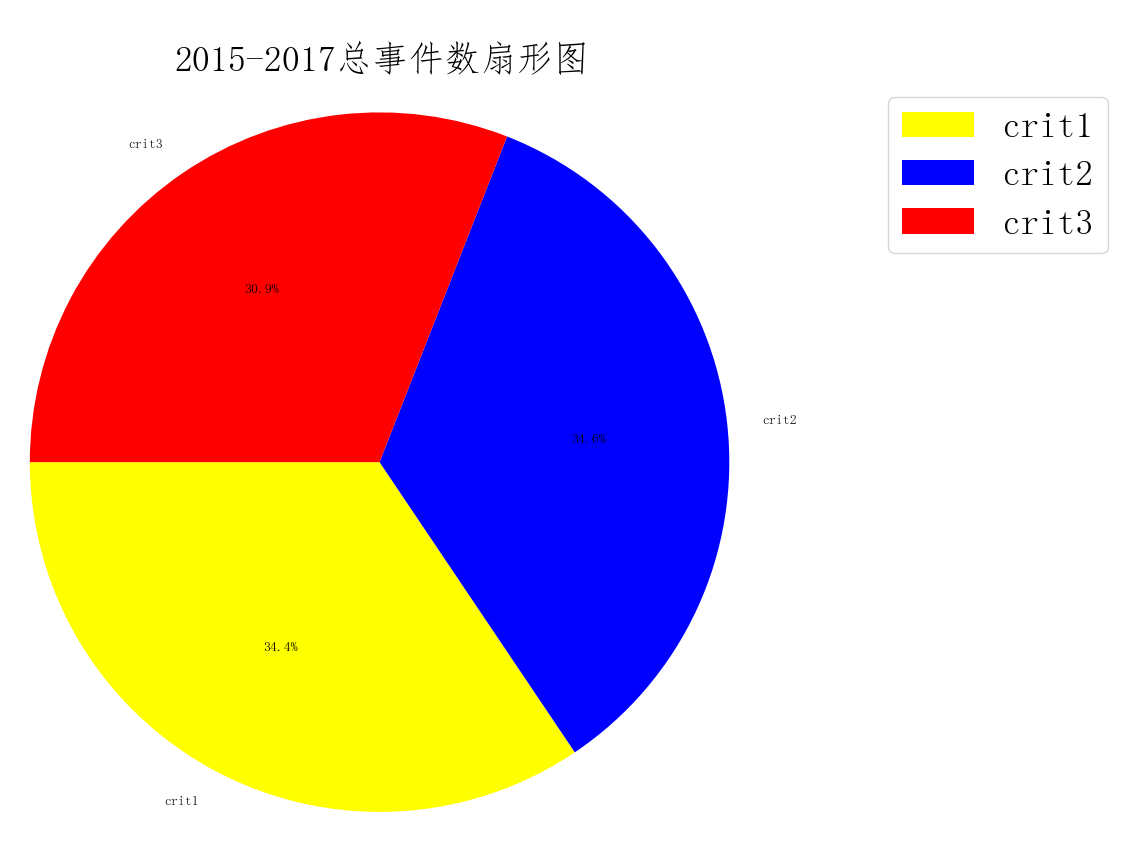
\includegraphics[width=.5\textwidth]{figures//img//Figure_12.png}
    }
    \subfigure{
        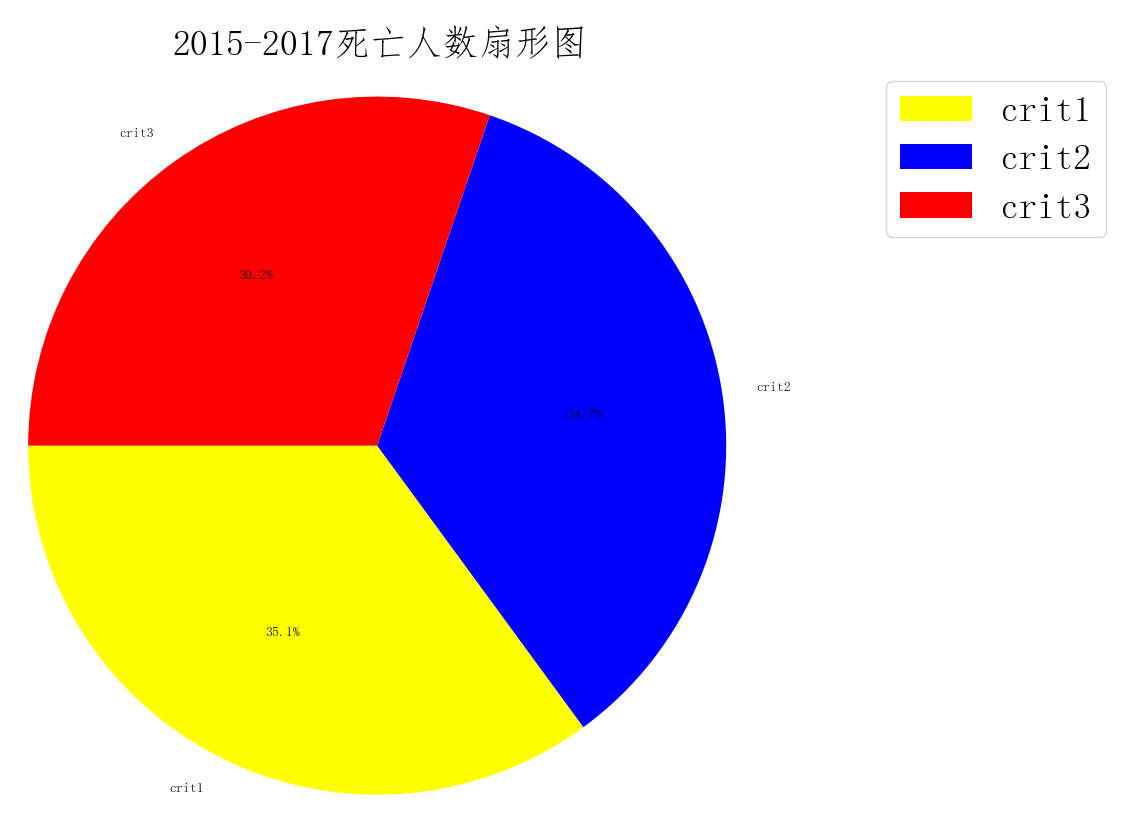
\includegraphics[width=.5\textwidth]{figures//img//Figure13.png}
    }
    \subfigure{
        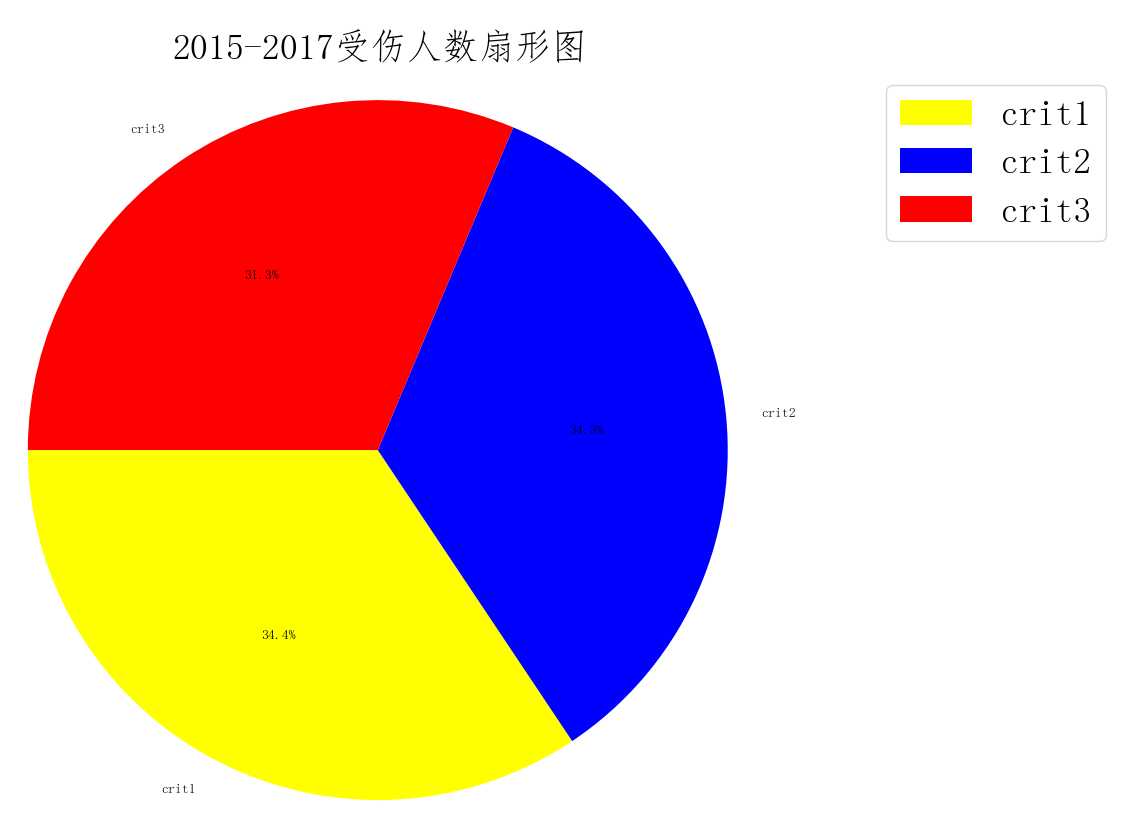
\includegraphics[width=.5\textwidth]{figures//img//Figure_14.png}
    }
    \subfigure{
        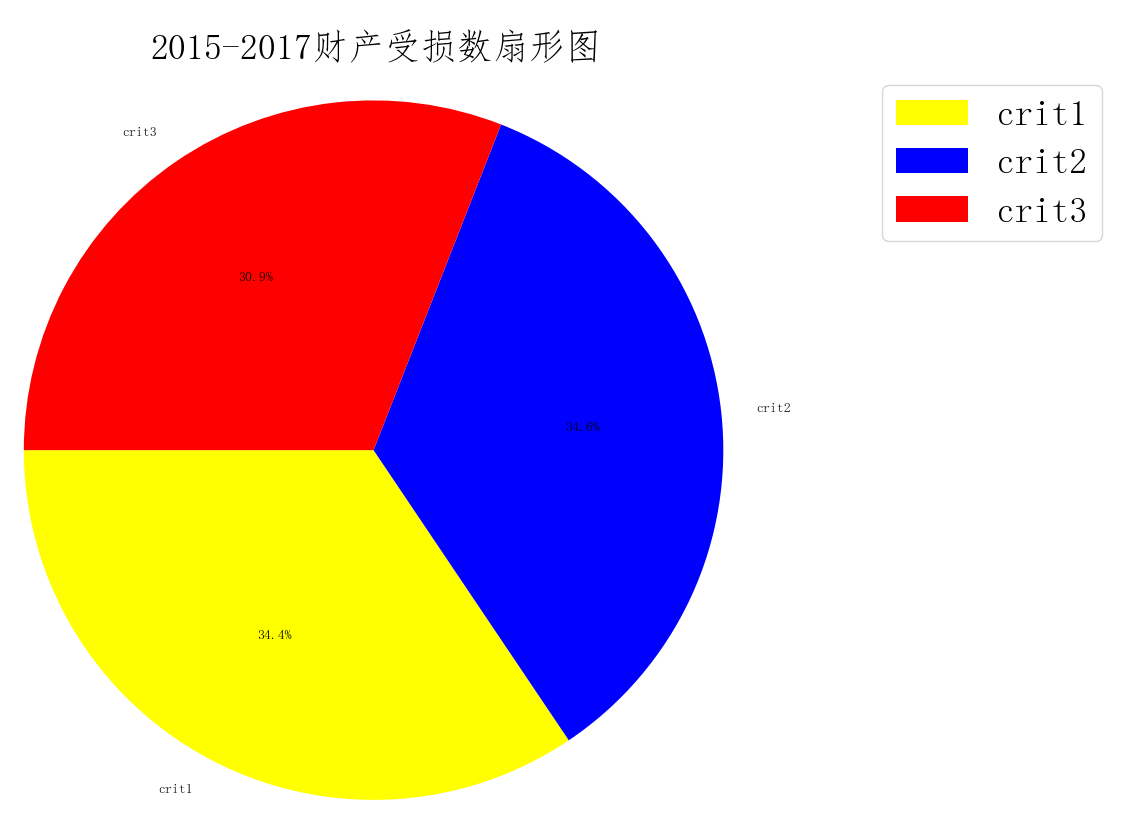
\includegraphics[width=.5\textwidth]{figures//img//Figure_15.png}
    }
    \caption{入选标准统计图}
    \label{tab:入选标准}
\end{figure}

图\ref{tab:入选标准}表示近三年恐怖袭击事件发生的入选标准分布图,
从恐怖袭击次数,死亡人数,伤亡人数和财产损失四个方面对入选标准进行统计。
从图中可以看到,标准1:政治、经济、宗教或社会目标(crit1)、
标准2:意图胁迫、恐吓或煽动更多的群众(crit2)、
标准3:超出国际人道主义法律范围(crit3)这些都是影响恐怖袭击事件的重要因素,
都是非常重要的。所以我们平时需要注意这些,从而才能使得恐怖袭击事件得到控制。

然后,我们对近三年的恐怖袭击发生的次数,死亡人数,
伤亡人数和财产损失属性和地区进行了统计,结果如图\ref{tab:地区统计}
从该图中,可以看到近三年中东和北非以及南亚地区都是恐怖袭击事件的高发地区。
死亡人数和财产损失也都是比较高的。
\begin{figure}[htbp]
    \subfigure{
        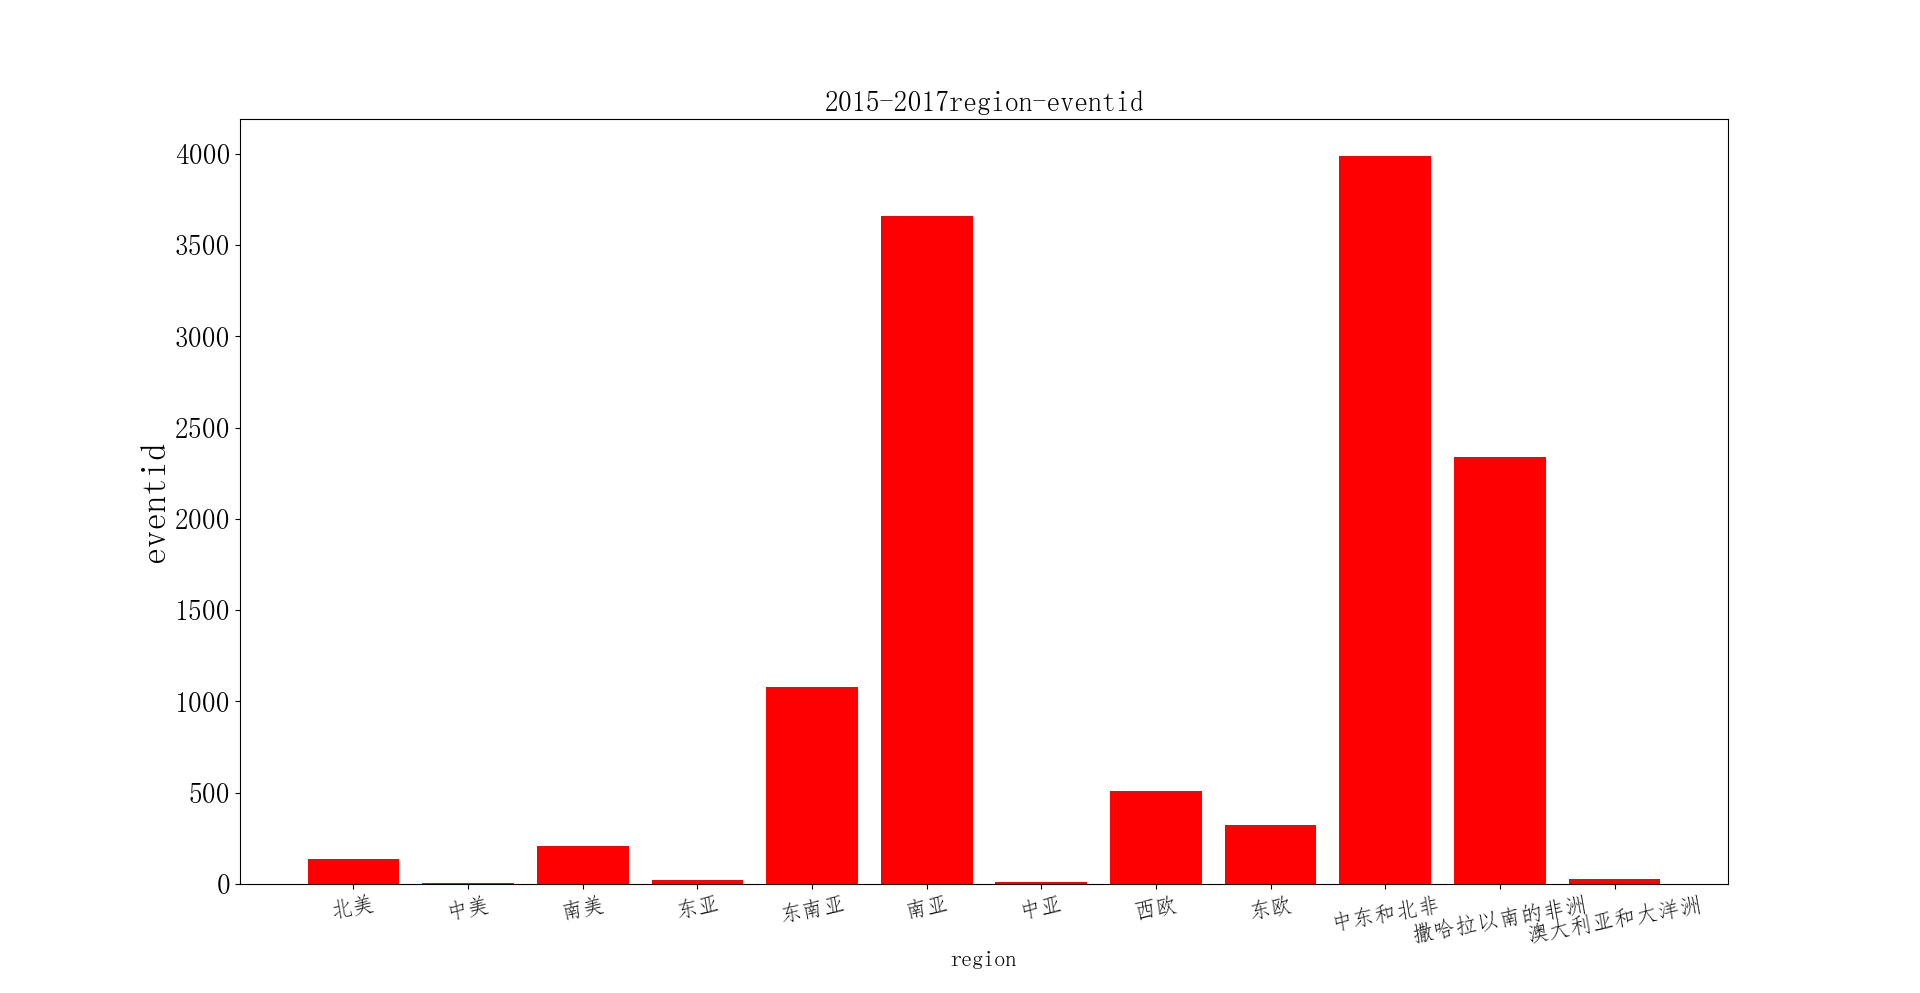
\includegraphics[width=.5\textwidth]{figures//img//Figure21.png}
    }
    \subfigure{
        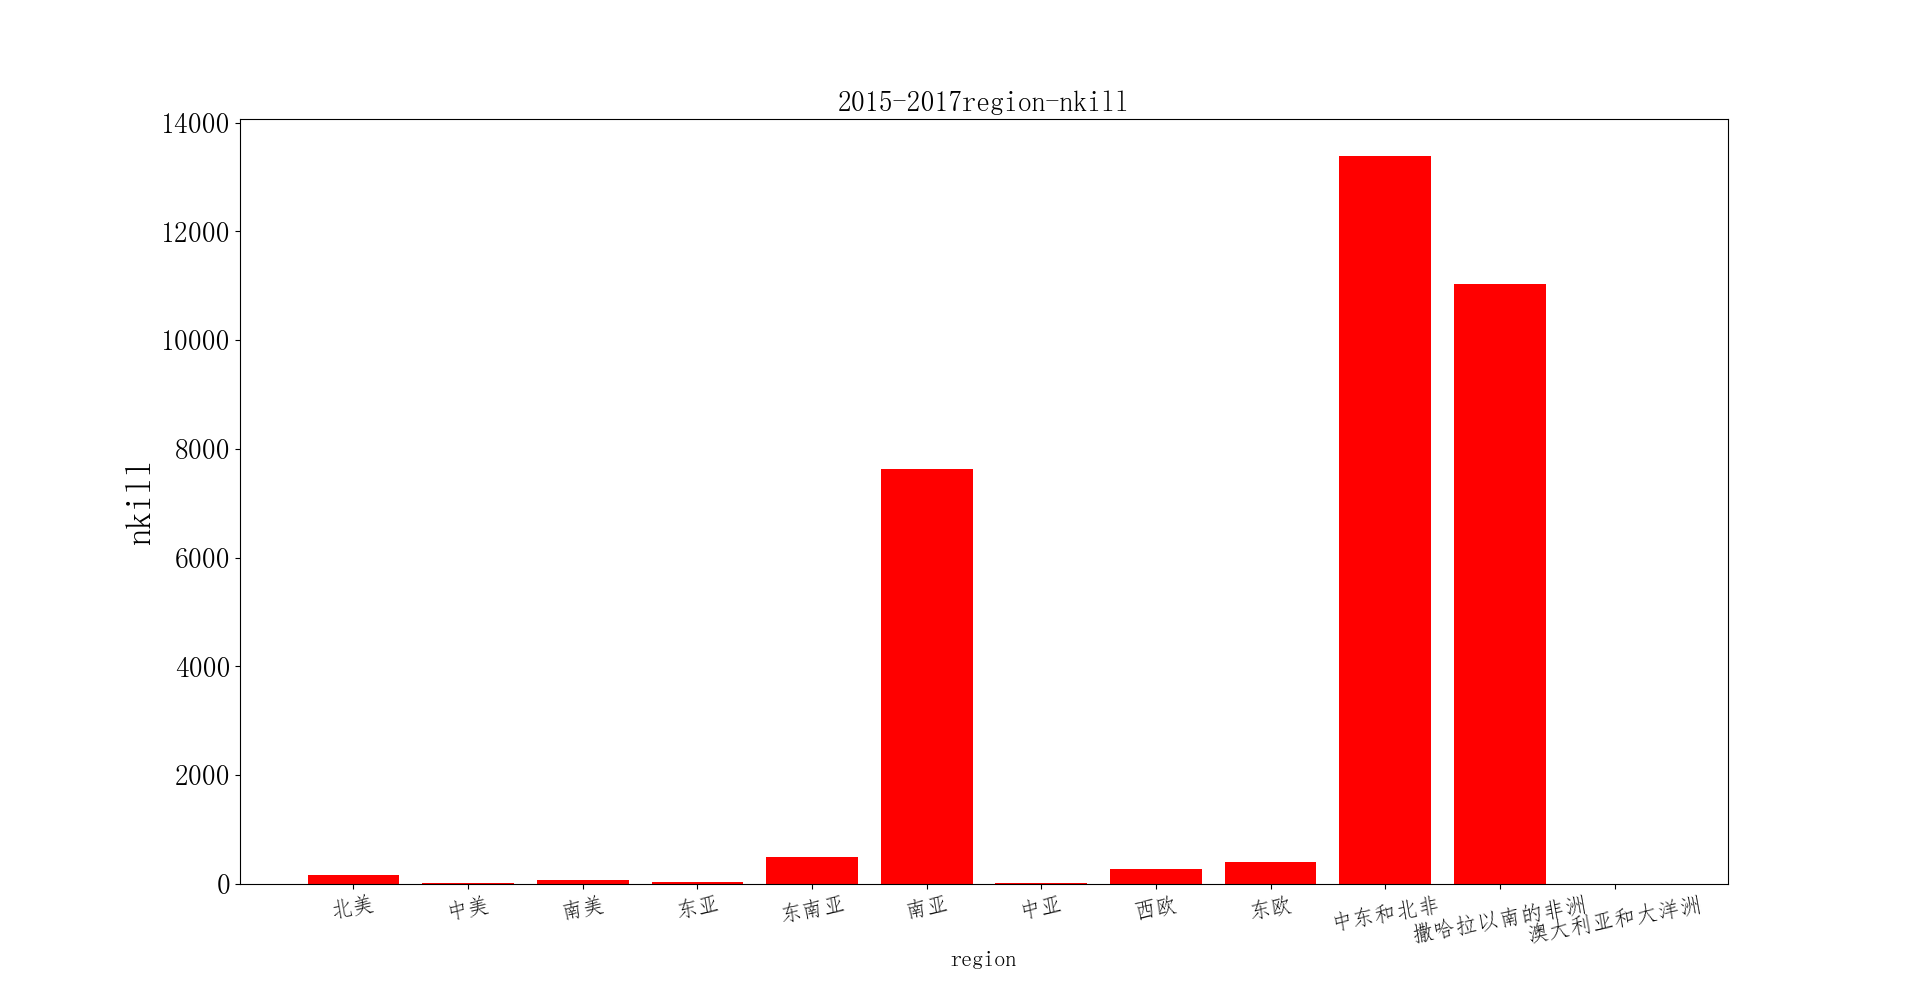
\includegraphics[width=.5\textwidth]{figures//img//Figure22.png}
    }
    \subfigure{
        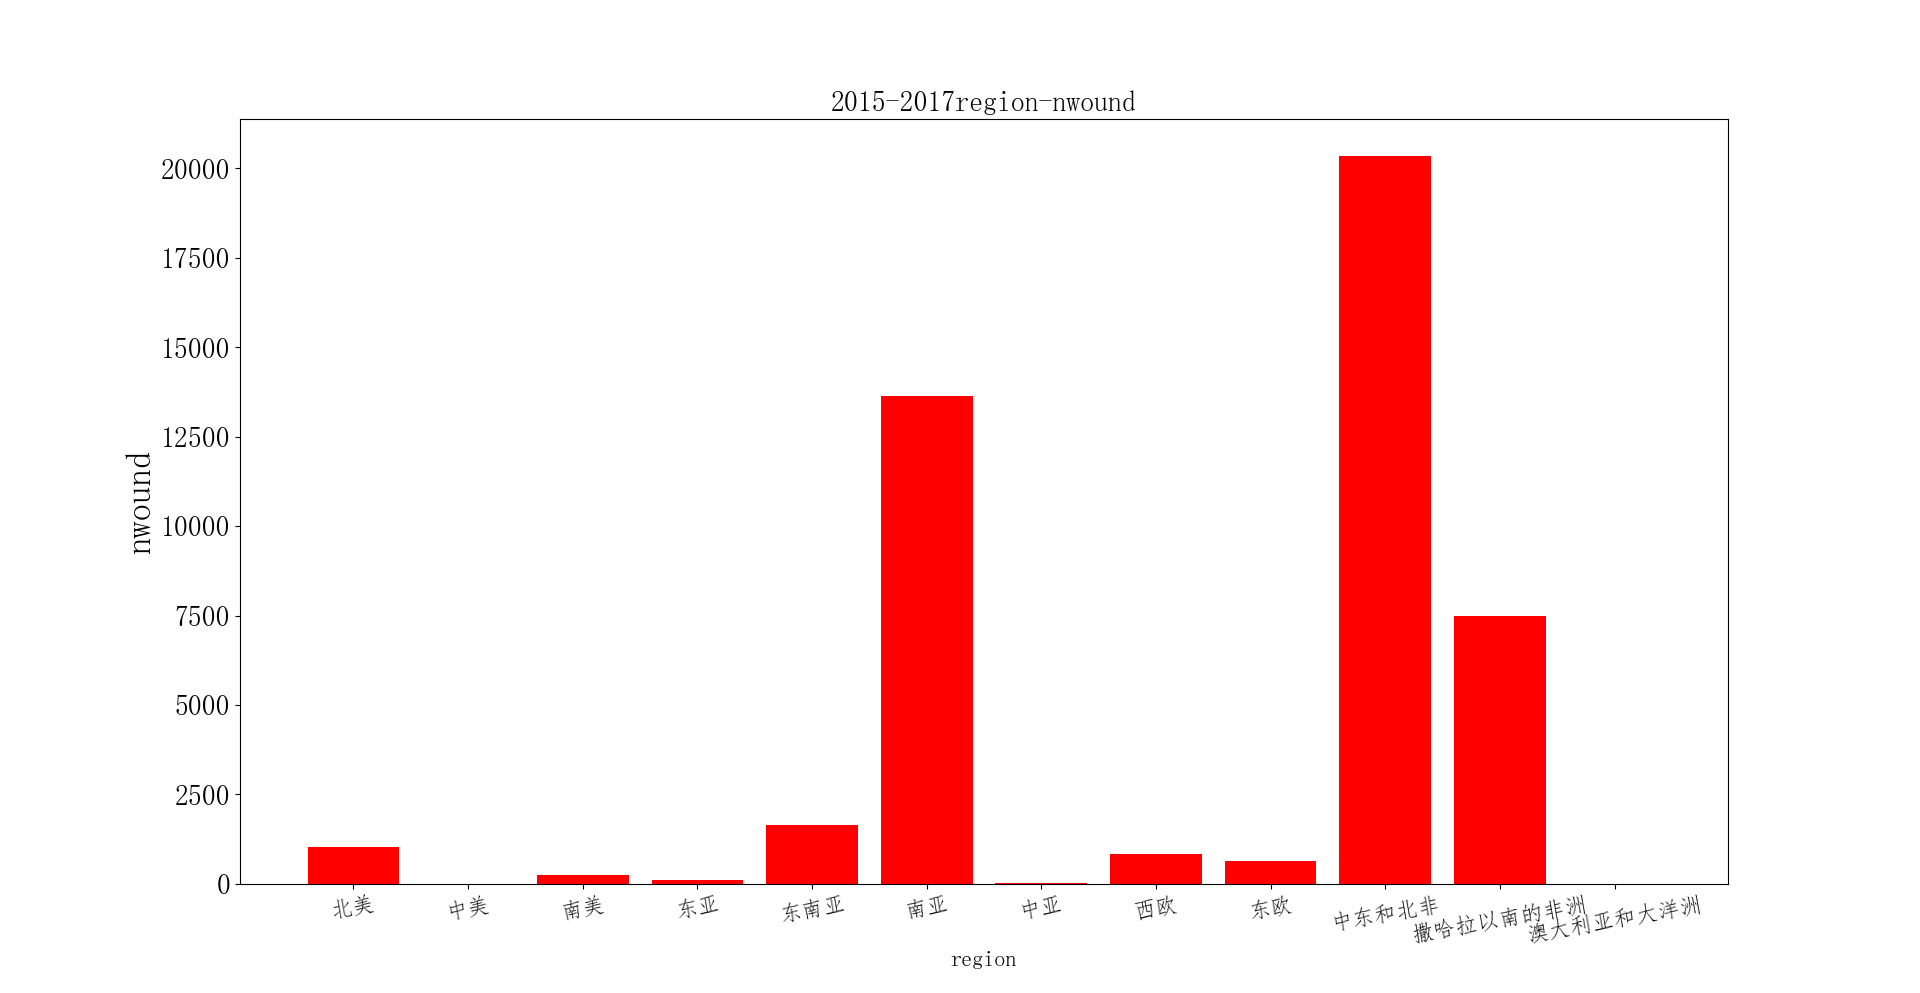
\includegraphics[width=.5\textwidth]{figures//img//Figure23.png}
    }
    \subfigure{
        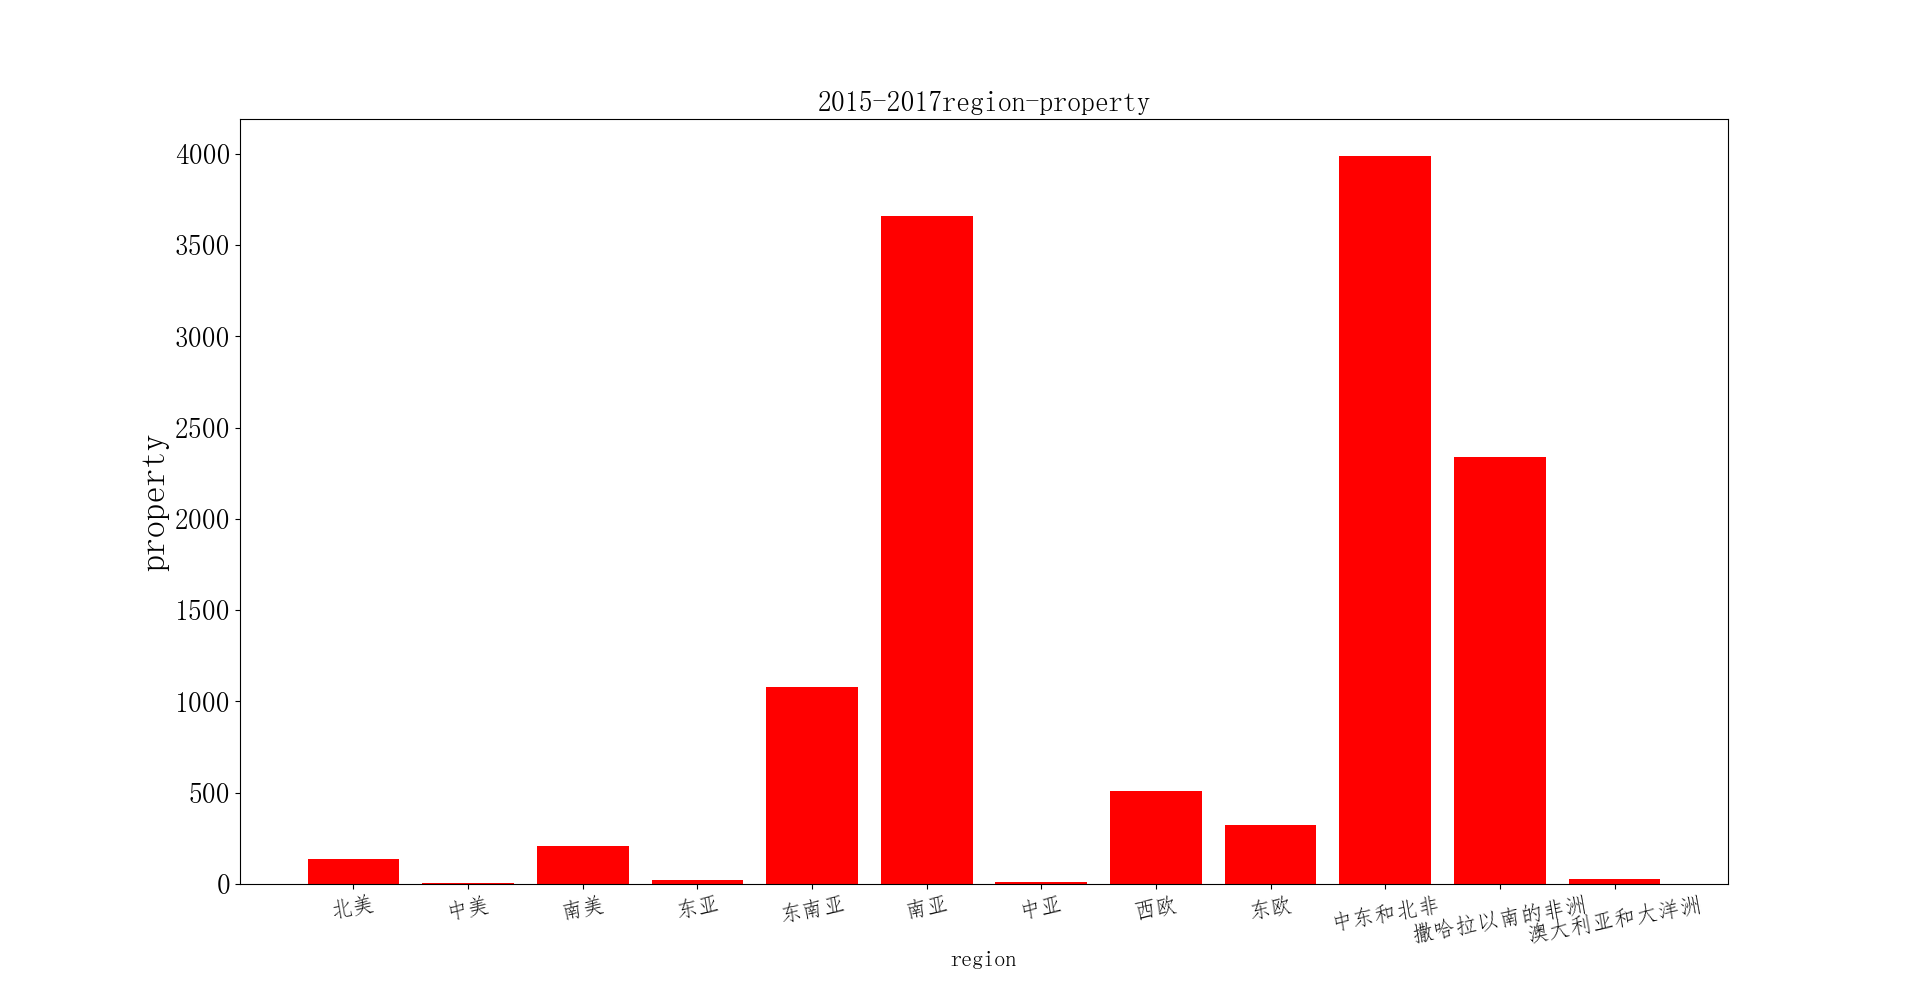
\includegraphics[width=.5\textwidth]{figures//img//Figure24.png}
    }
    \caption{地区统计}
    \label{tab:地区统计}
\end{figure}

对近三年的恐怖袭击事件发生的时间和恐怖袭击事件发生的次数,
死亡人数,伤亡人数和财产损失进行了统计,结果如图\ref{tab:时空统计}
\begin{figure}[htbp]
    \subfigure{
        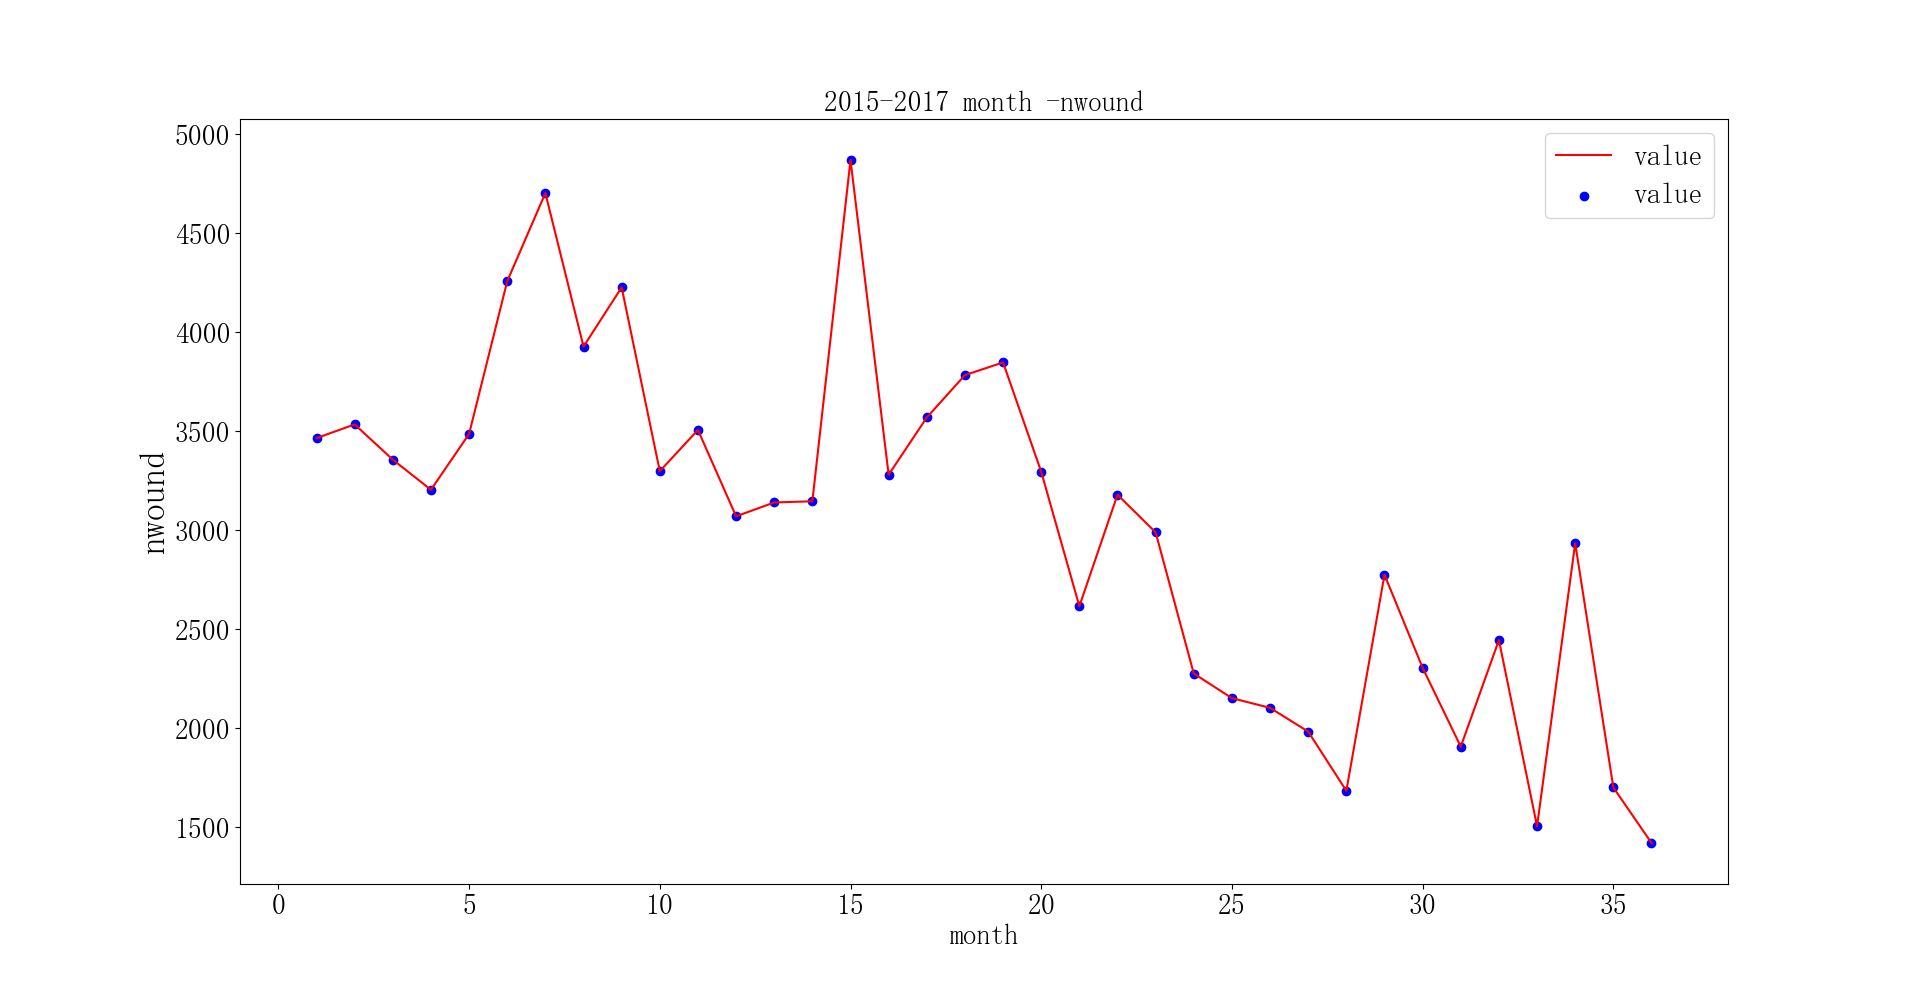
\includegraphics[width=.5\textwidth]{figures//img//Figure3-1.png}
    }
    \subfigure{
        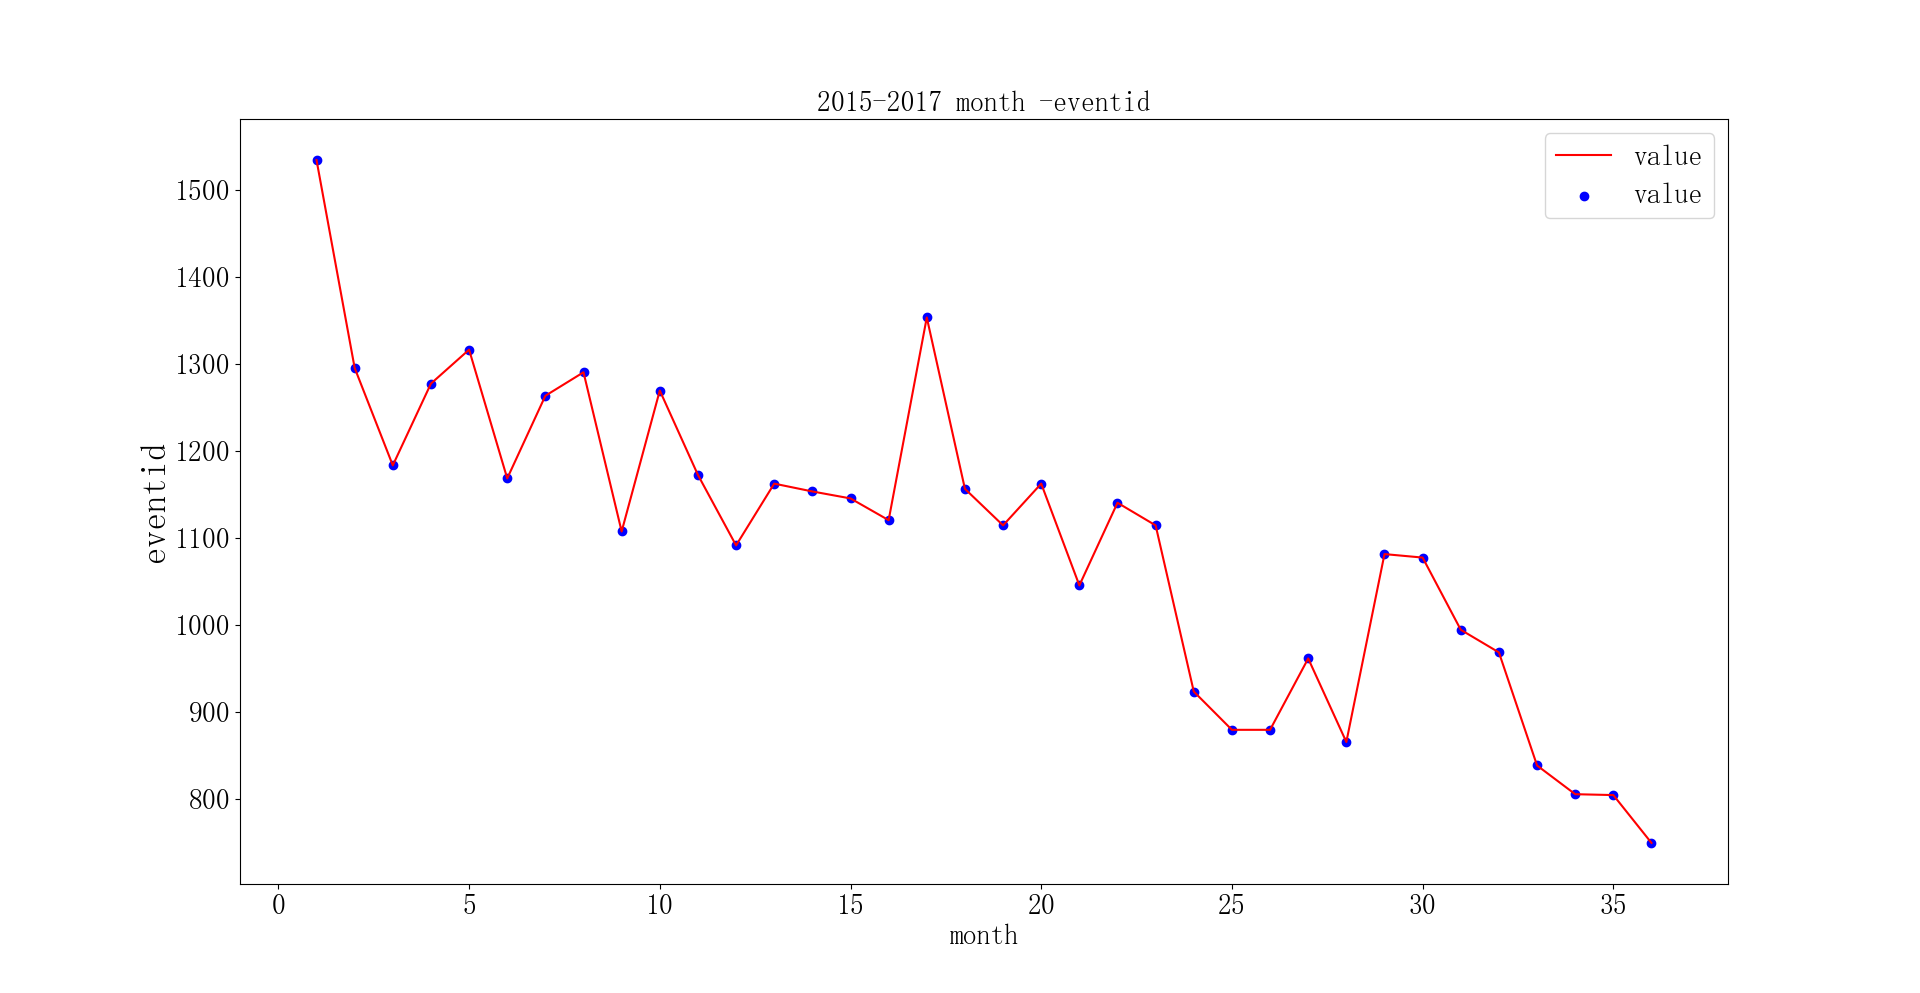
\includegraphics[width=.5\textwidth]{figures//img//Figure3-2.png}
    }
    \subfigure{
        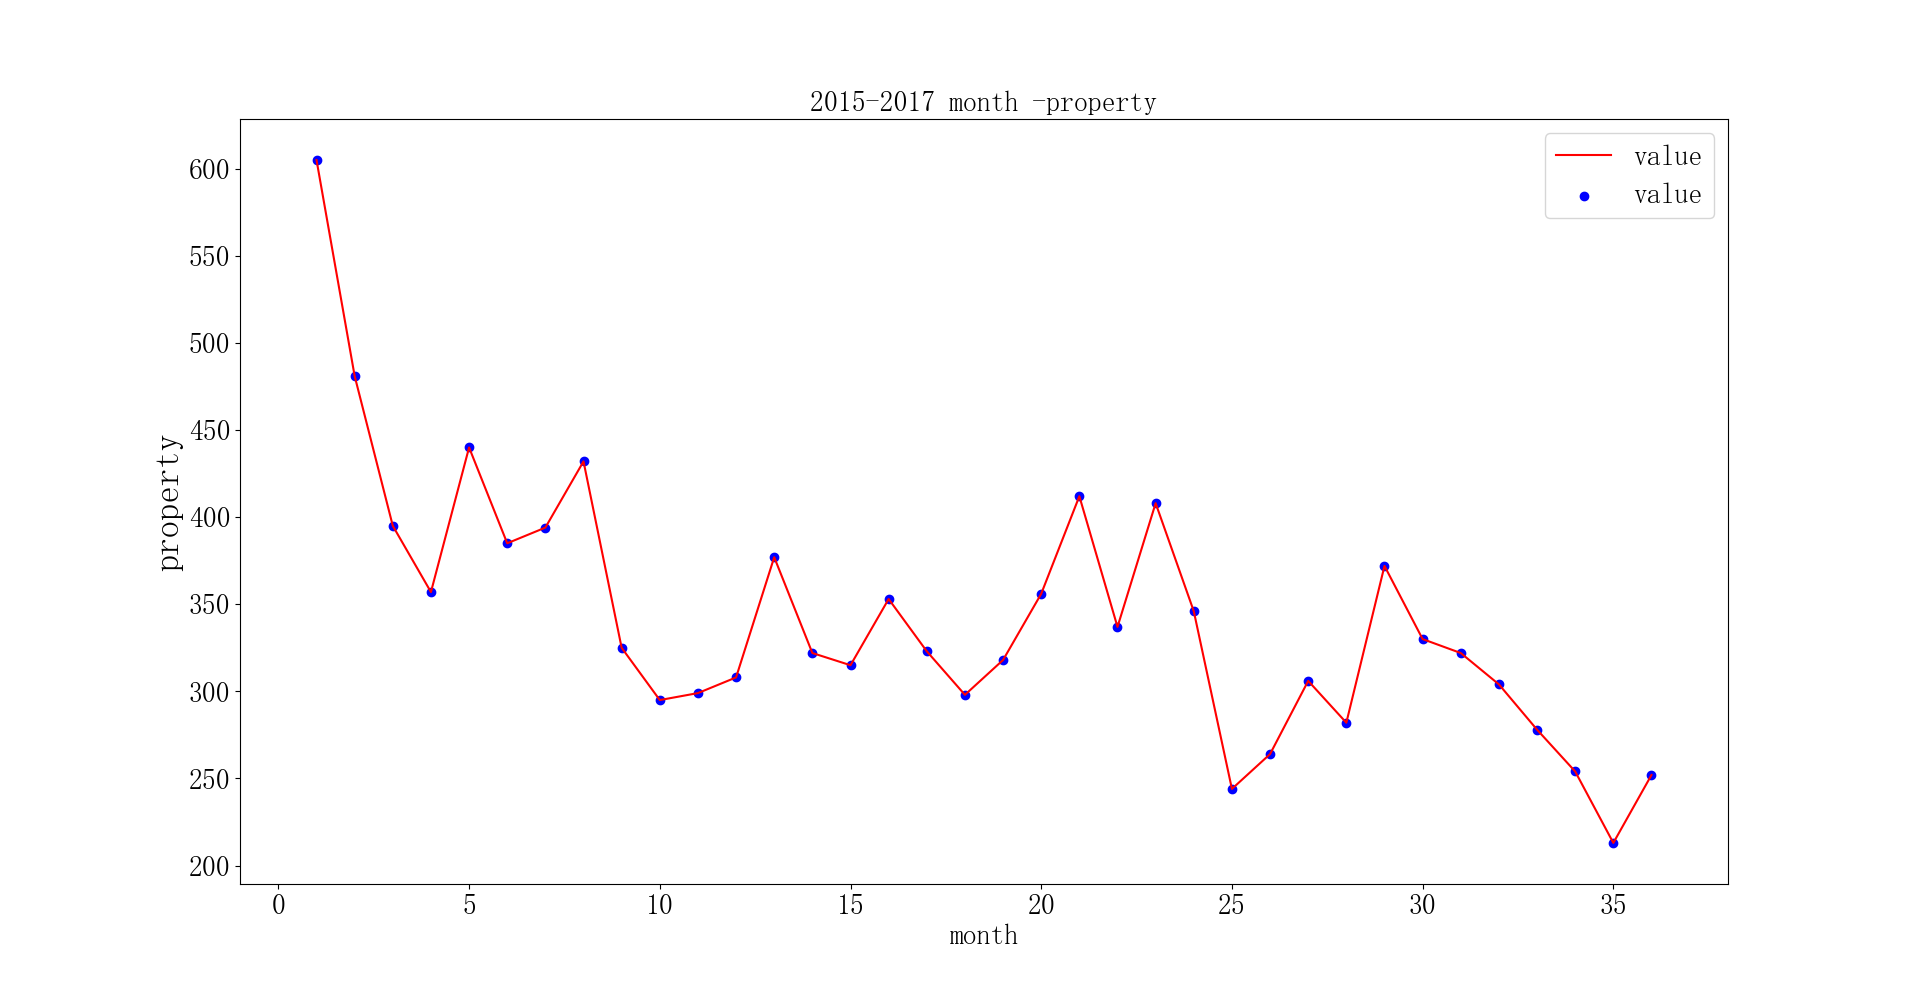
\includegraphics[width=.5\textwidth]{figures//img//Figure3-3.png}
    }
    \subfigure{
        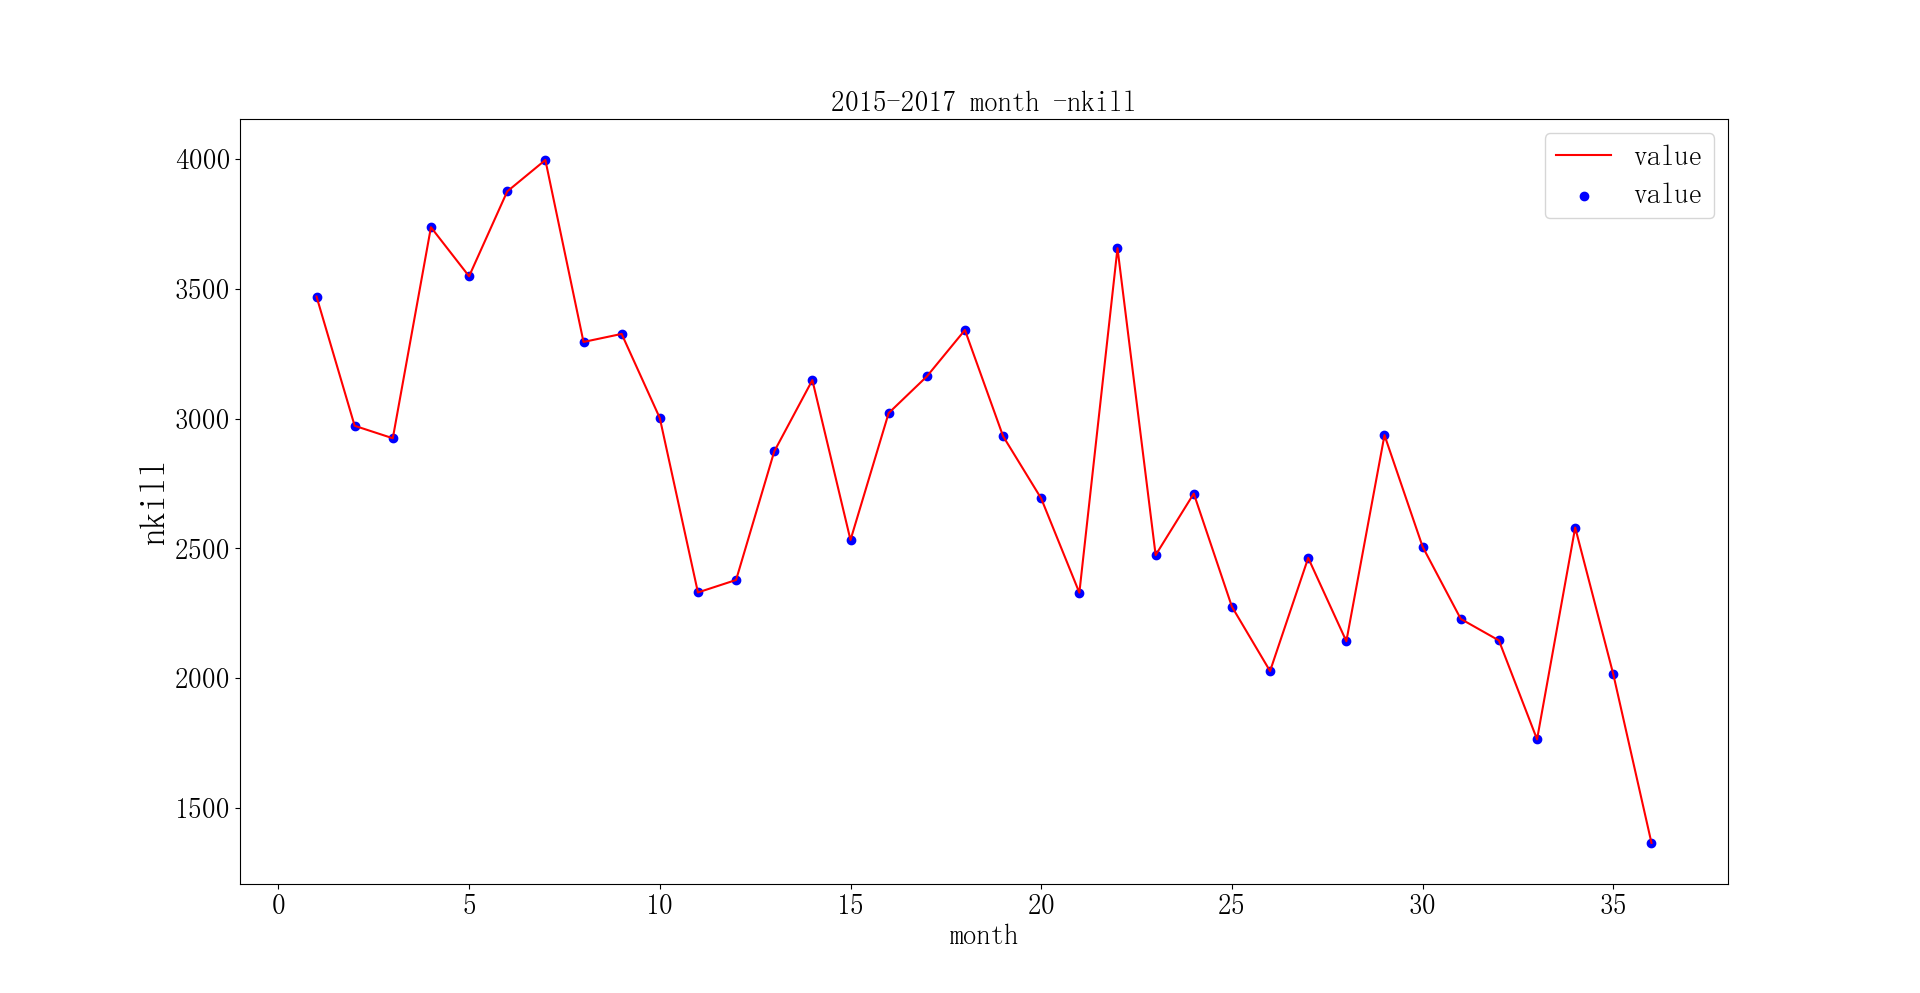
\includegraphics[width=.5\textwidth]{figures//img//Figure3-4.png}
    }
    \caption{时空特性}
    \label{tab:时空统计}
\end{figure}

对近三年的恐怖袭击事件的危害程度的层级分布进行了统计,结果如图\ref{tab:级别分布}
\begin{figure}[htbp]
    \subfigure{
        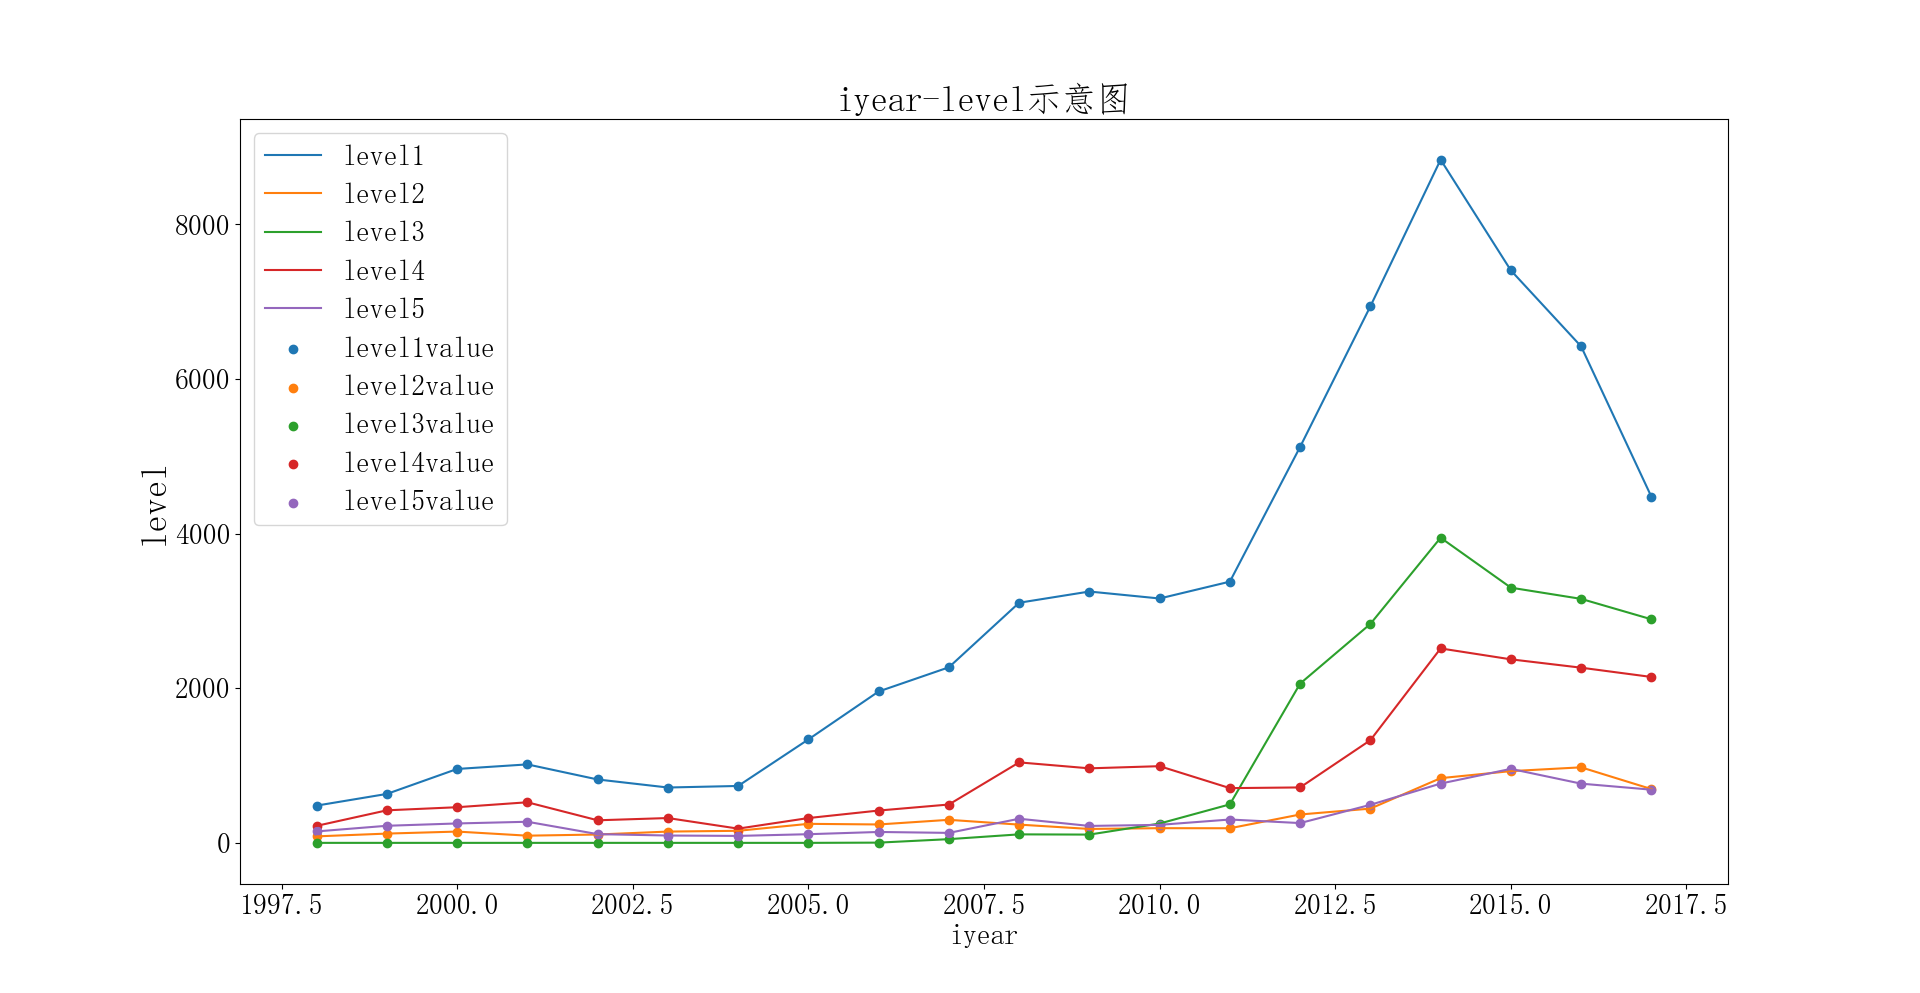
\includegraphics[width=.5\textwidth]{figures//img//Figure_4-3.png}
    }
    \subfigure{
        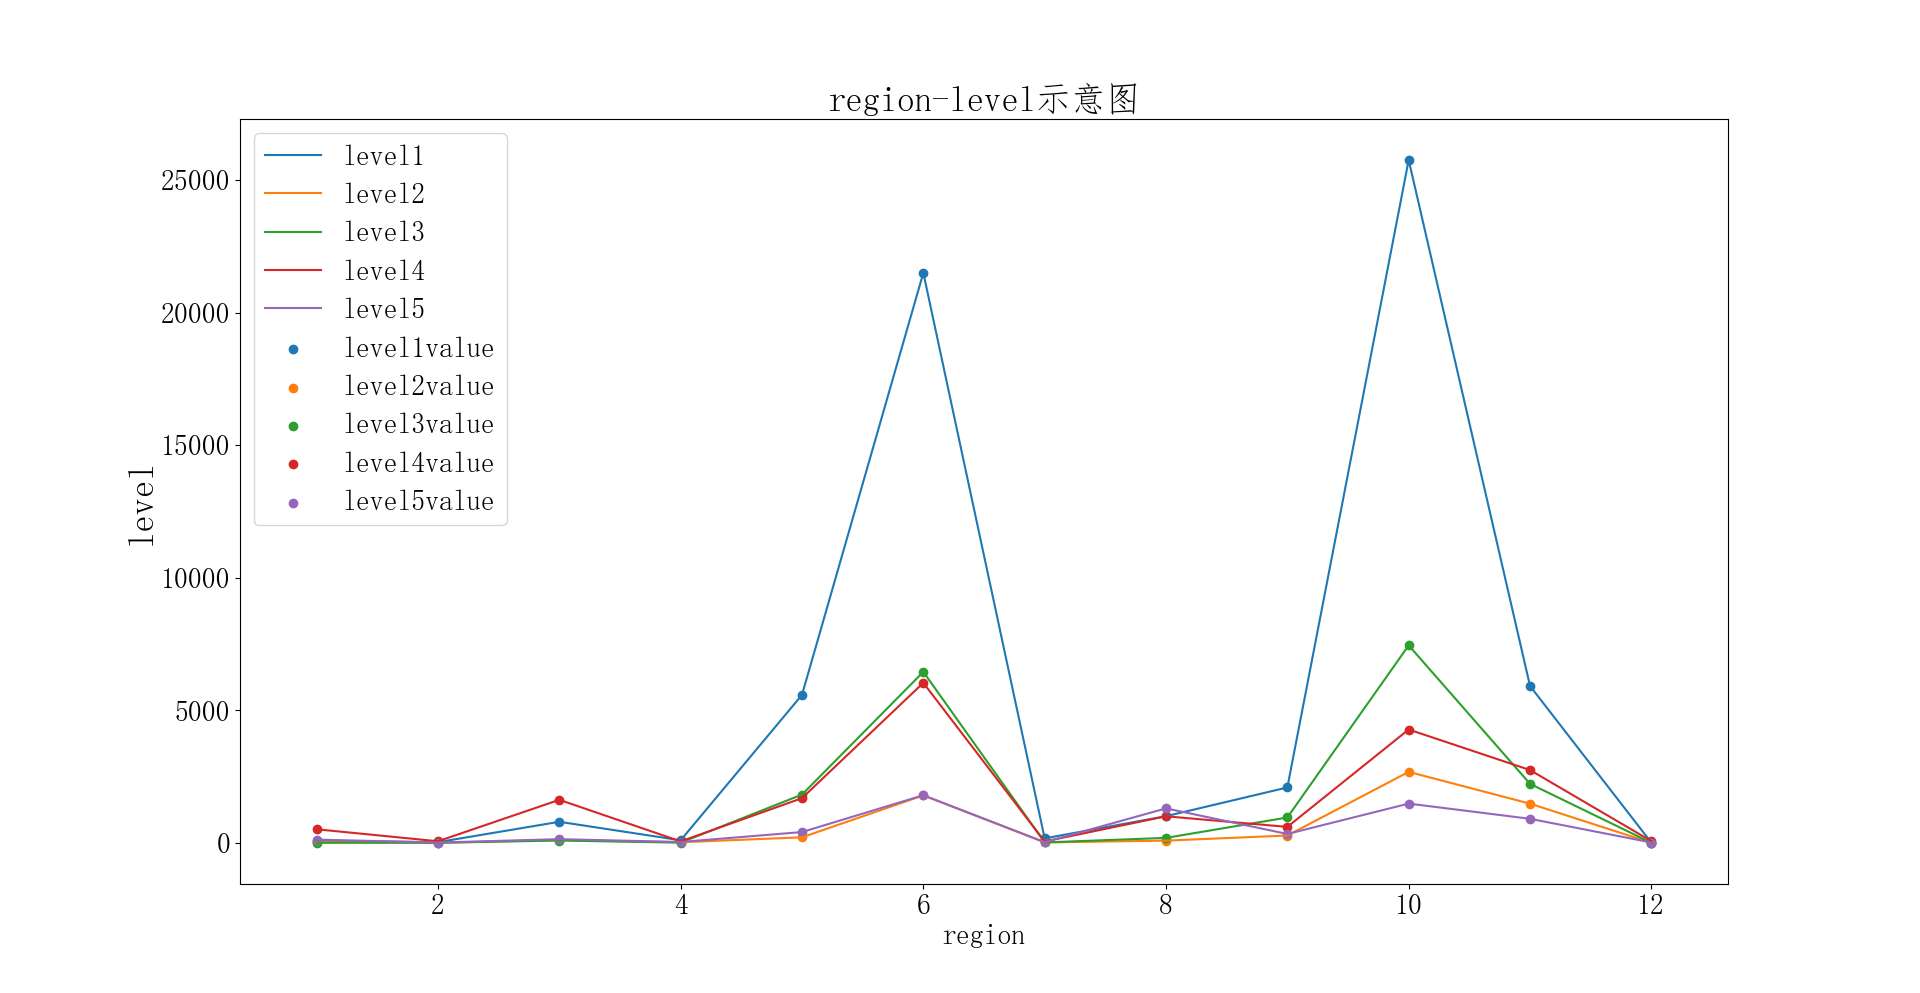
\includegraphics[width=.5\textwidth]{figures//img//Figure_4-4.png}
    }
    \caption{级别分布图}
    \label{tab:级别分布}
\end{figure}



\begin{figure}[htbp]
    \subfigure{
        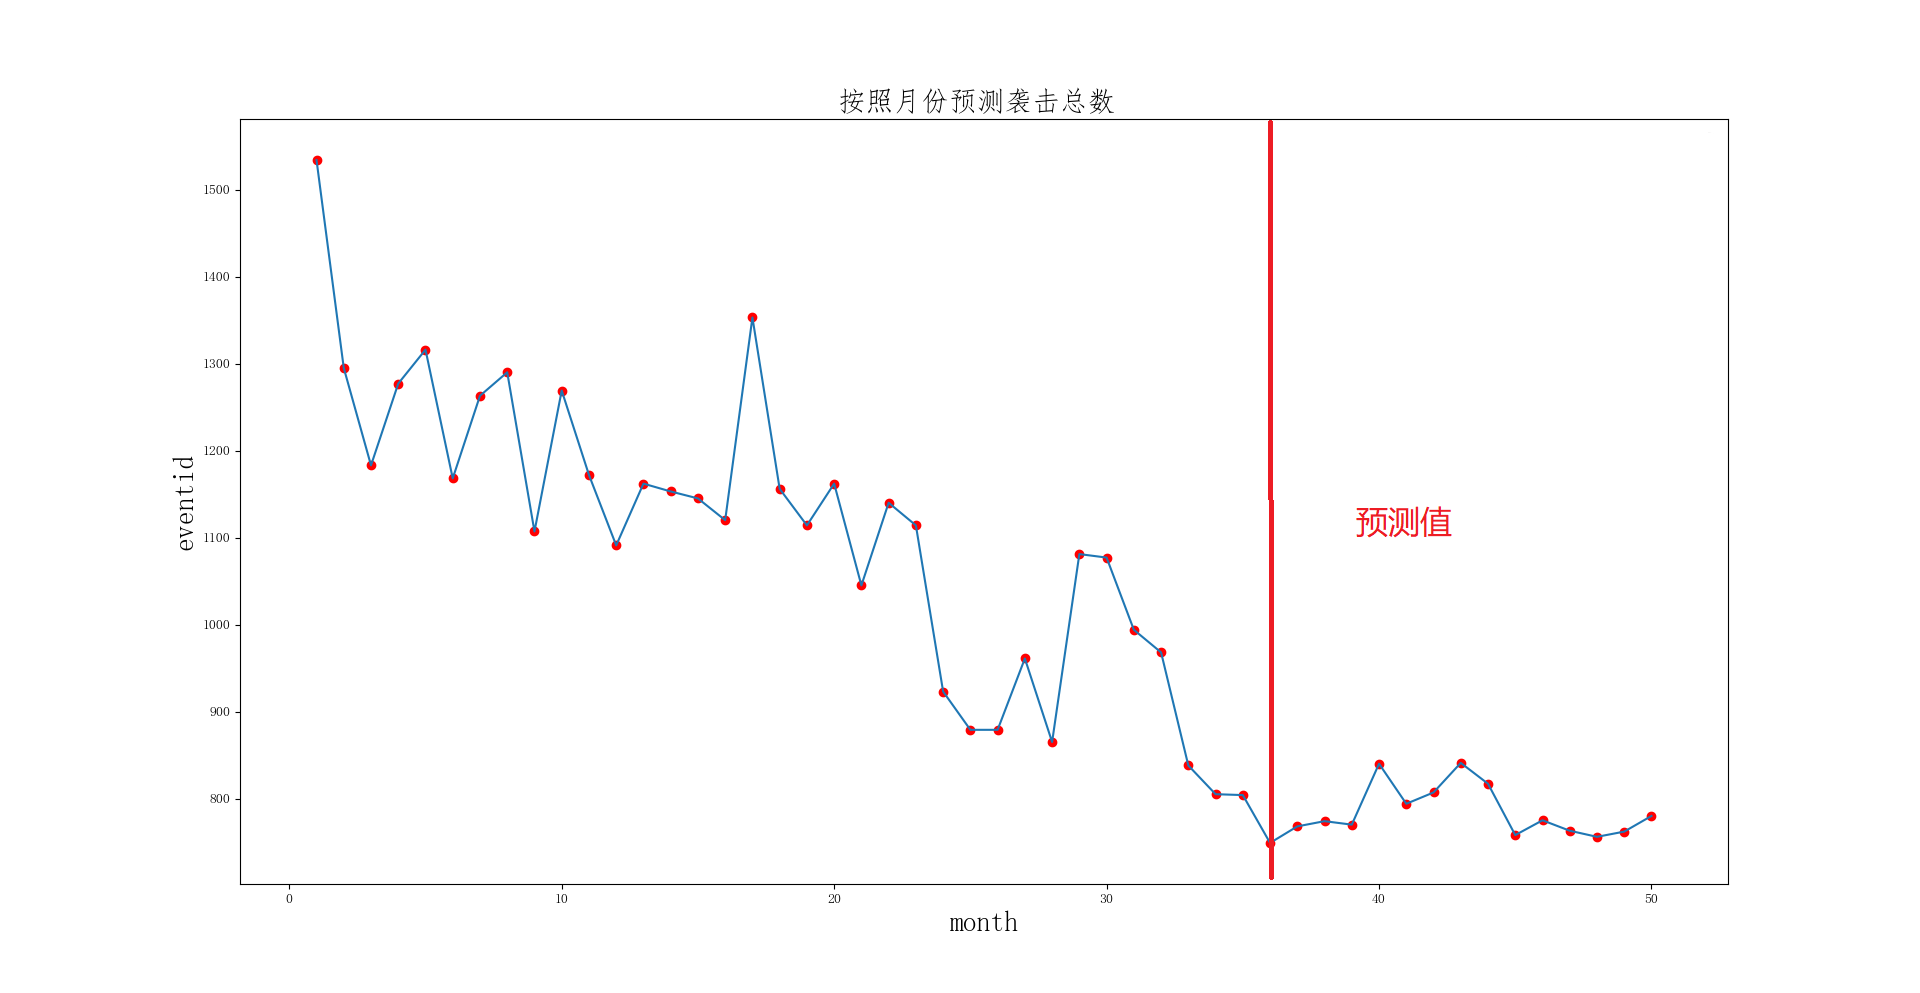
\includegraphics[width=.5\textwidth]{figures//img//Figure_51.png}
    }
    \subfigure{
        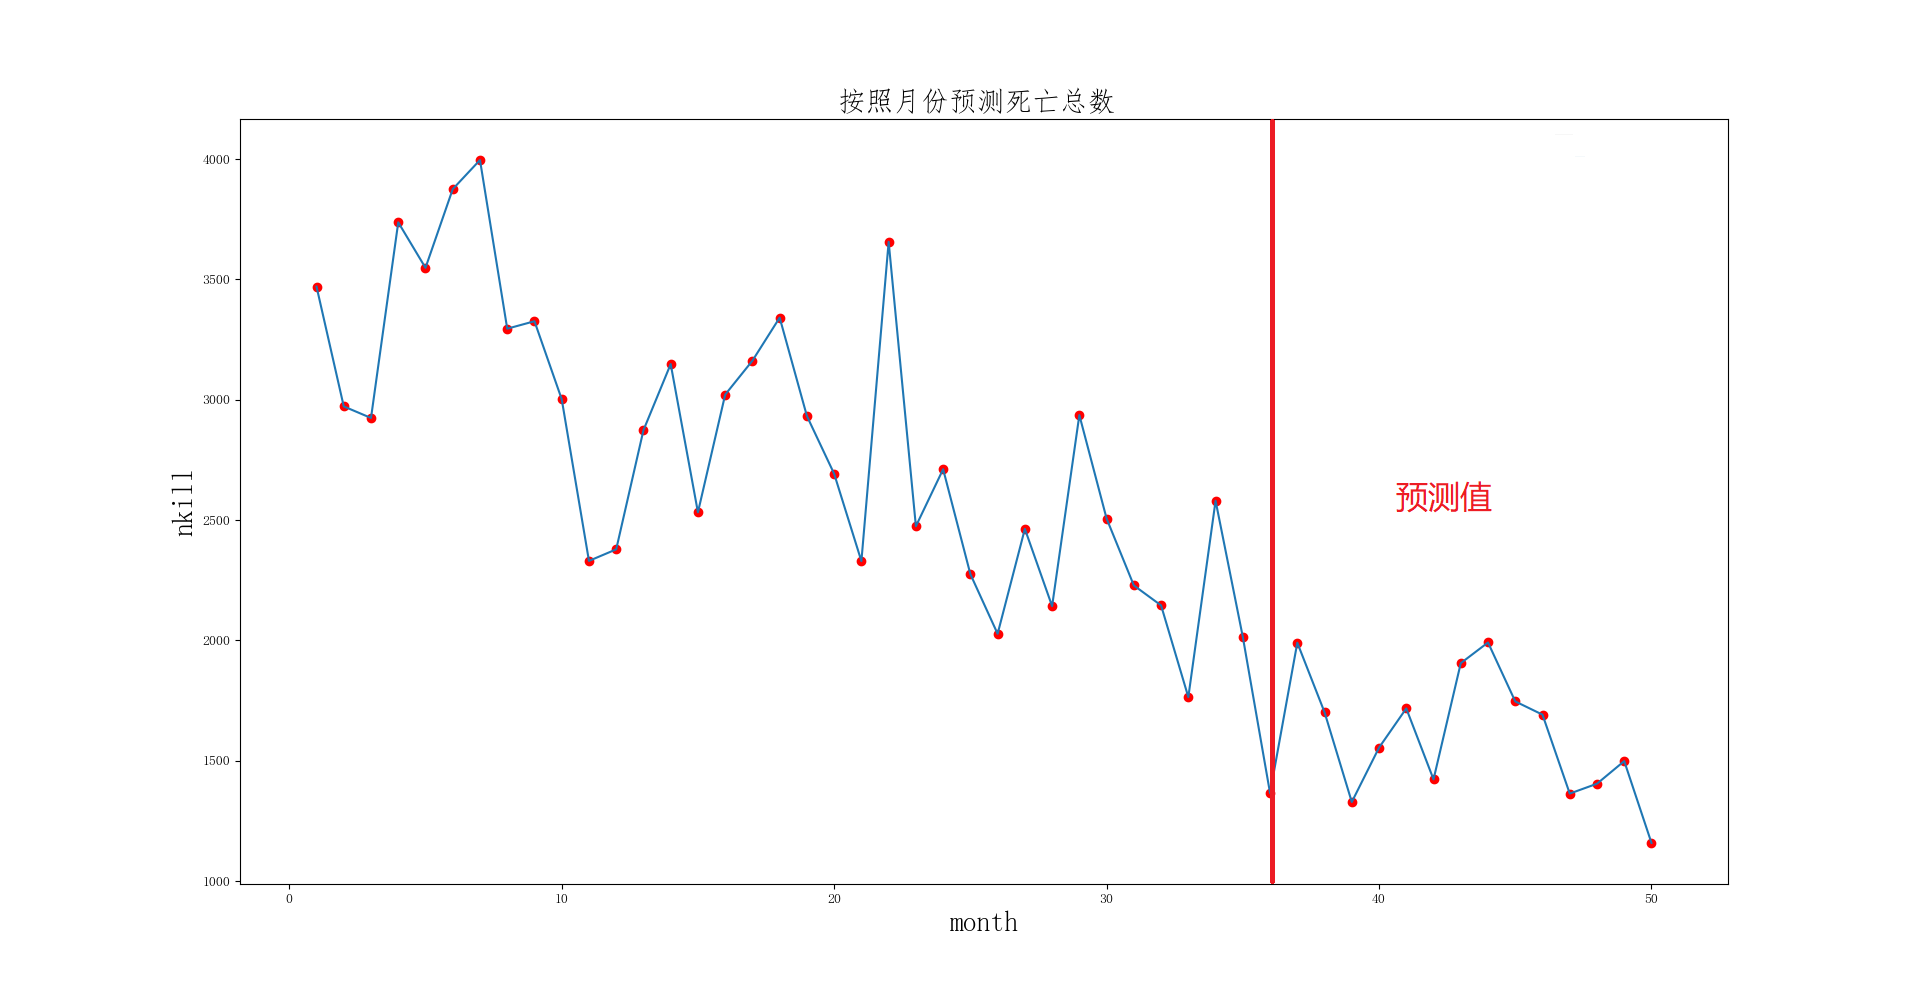
\includegraphics[width=.5\textwidth]{figures//img//Figure_52.png}
    }
    \subfigure{
        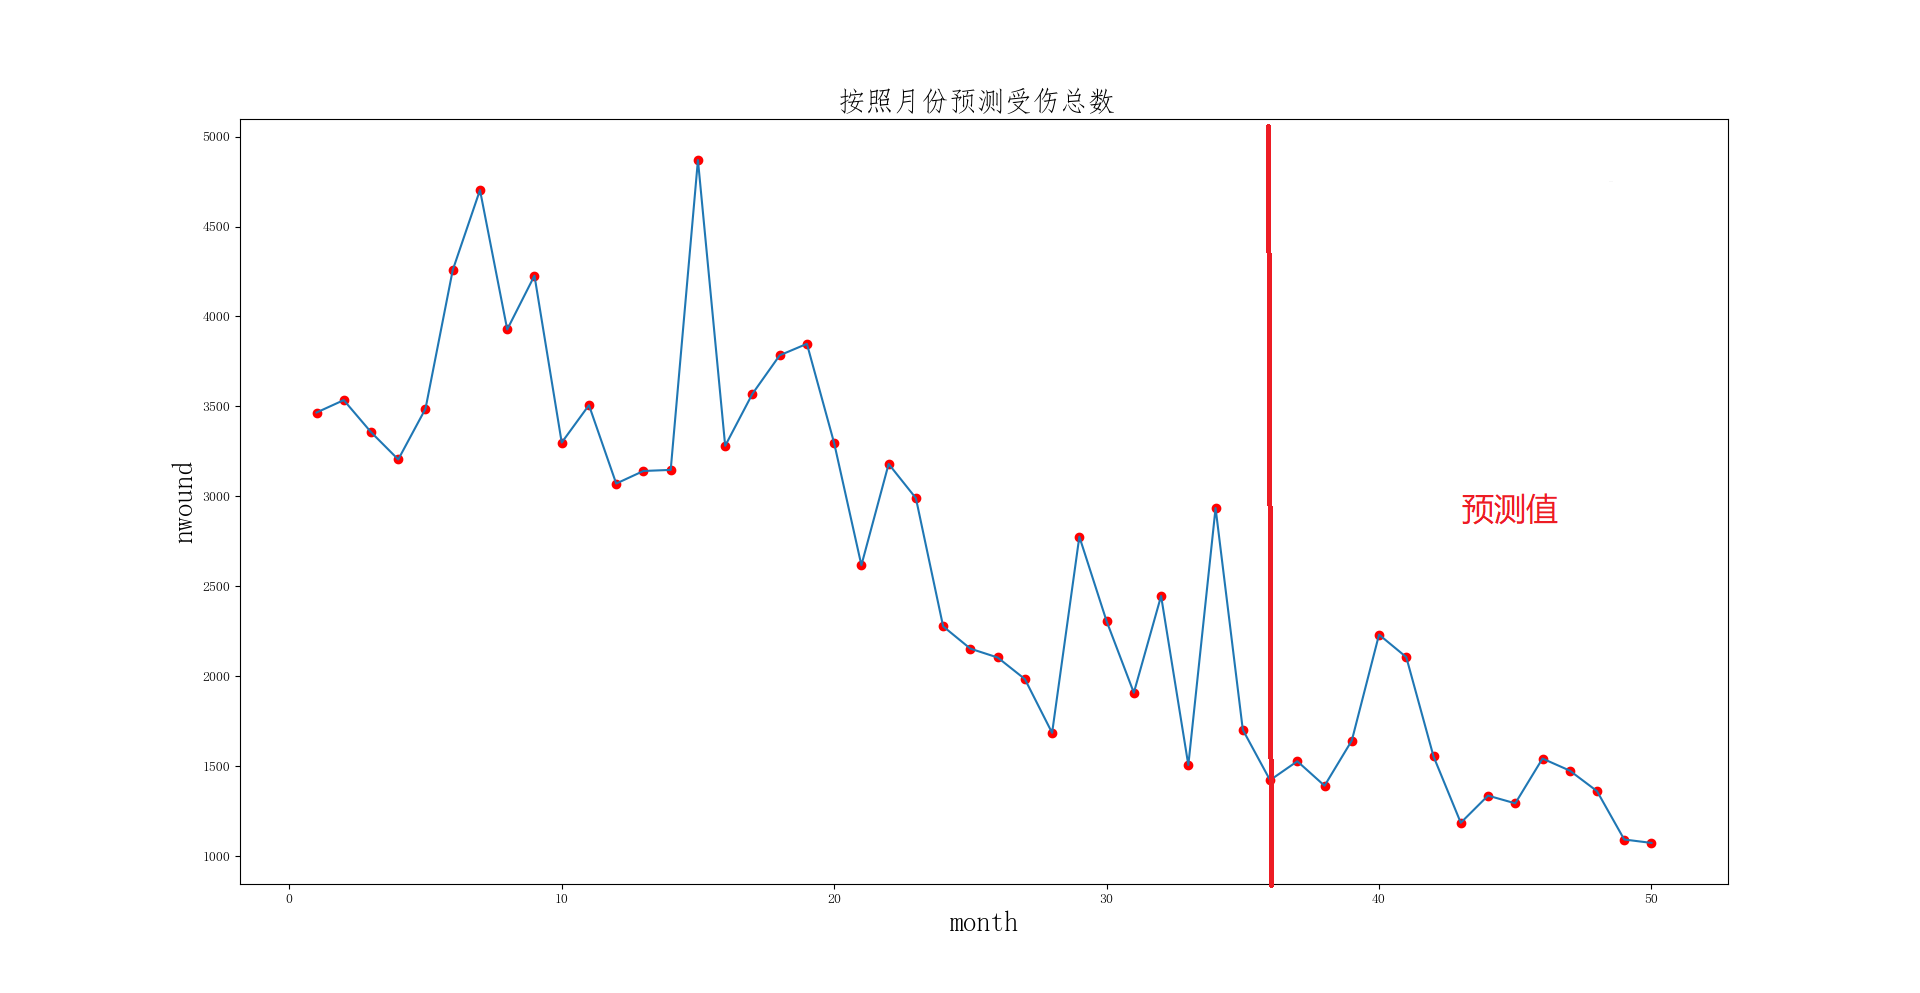
\includegraphics[width=.5\textwidth]{figures//img//Figure_53.png}
    }
    \subfigure{
        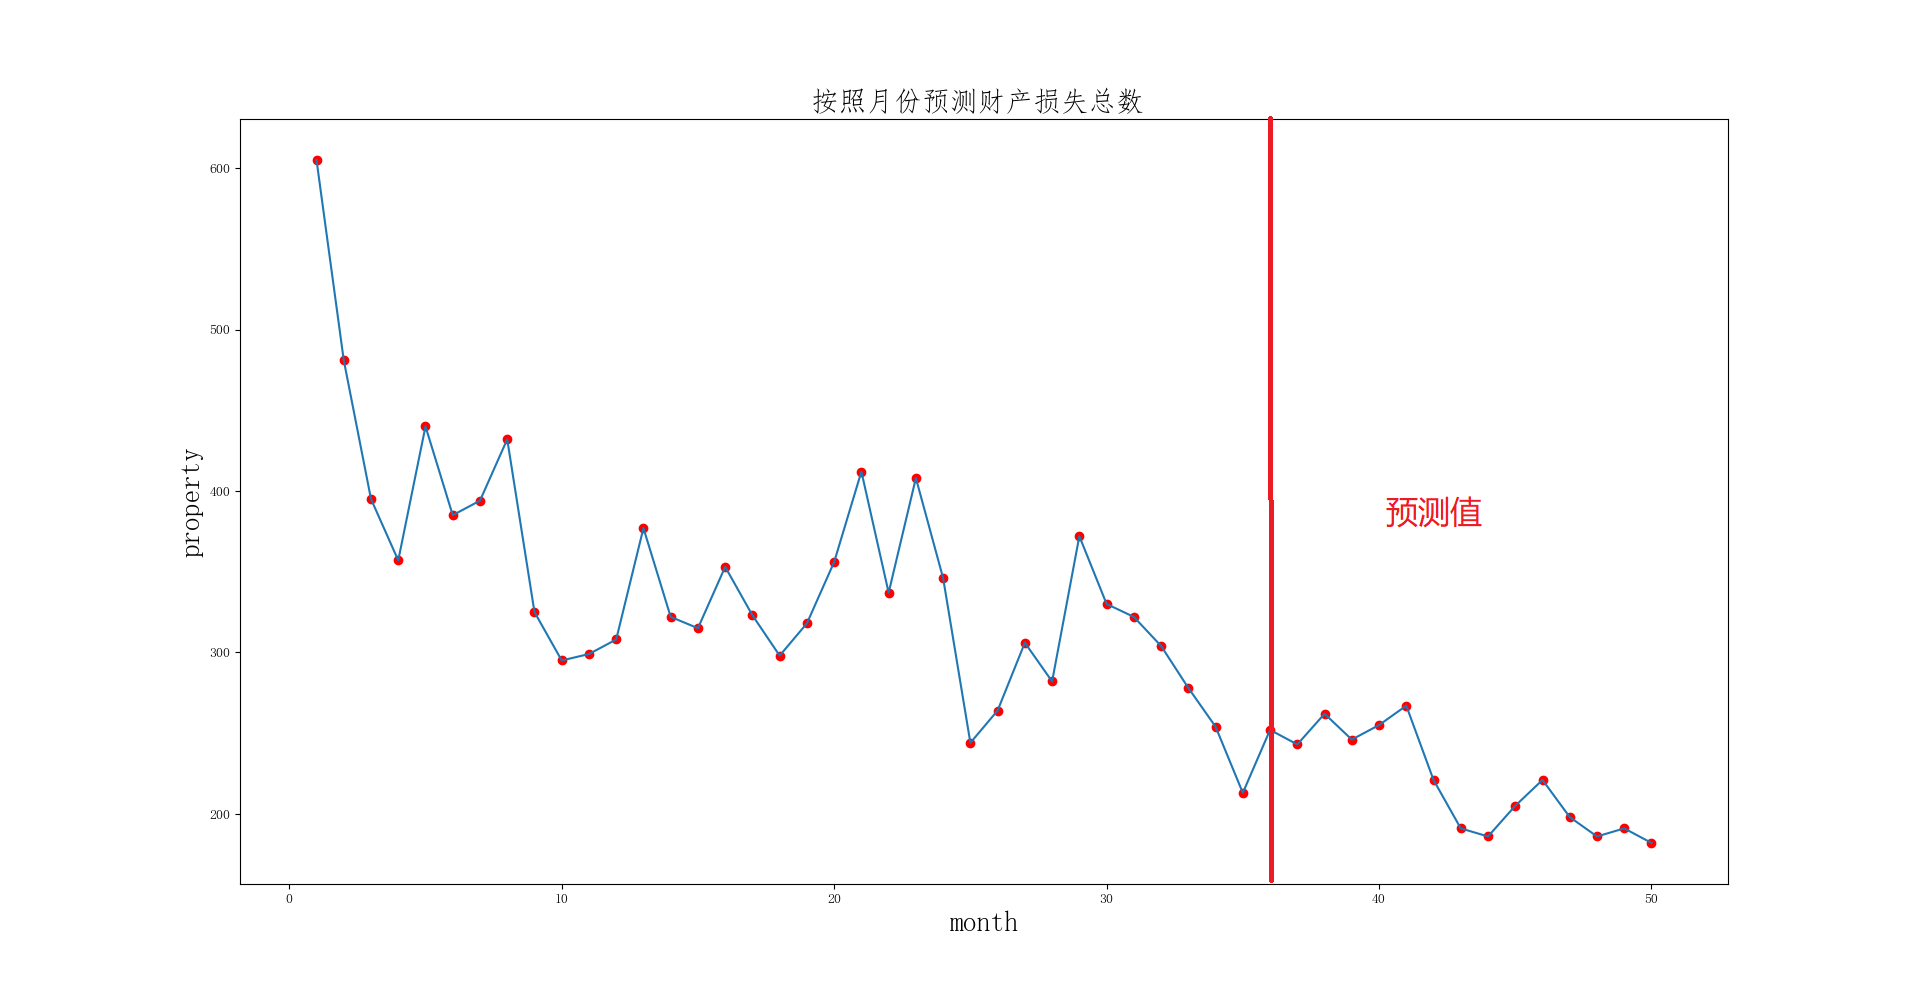
\includegraphics[width=.5\textwidth]{figures//img//Figure_54.png}
    }
    \caption{时空特性预测图}
    \label{tab:result}
\end{figure}

图\ref{tab:result}通过XGBoost算法建模,对袭击事件发生次数,
死亡人数,受伤人数和财产损失的时空特性进行了预测。
可以看到,随着时间的推移,恐怖袭击次数是逐渐减少的。
同时也可以看到全球反恐态势愈来愈强,
这也同时反应了全球对于该事件的重视。
我们建议,国家和政府在反恐斗争中扮演着很重要的角色,
同时,教育对于一代又一代的人来说也是非常重要的,
所以需要从方方面面进行反恐斗争。
我们认为,反恐对于我们的生活是十分必要的,
因为恐怖袭击无论是对于我们的国家还是民族都是非常的抵触的,
人的生命只有一次,在这仅存的几十年时间里,
大家都应该珍惜自己的生命,同时也应该爱惜其他人的生命。


\section{模型评价及推广}

在本次数学建模中,
针对任务一,我们利用了高斯混合聚类模型,
KNN,XGBoost等模型分别来分类和预测。
通过聚类将无标签数据集分为五类,
然后利用香农熵来作为每个类的权值,
最终将整个数据集分为五类,
分别代表五个等级。
然后对所有事件按照等级排序,
得到最终的结果。
虽然很多参考文献中采用了主观方法进行分级,
但是我们除了利用参考文献中的参考变量,
还通过查阅资料,
获取到其他可能影响恐怖袭击事件分级危害性的因素。
最终将所有属性整合到一起,进行聚类,
计算权值进而求和的结果。
但是在这个过程中,有一些数据预处理的过程可能还会有更好的处理方法,
甚至在模型的建立和算法的选择上可能会有更好的方法。
这也是非常值得我们进一步做更多的研究的。

针对任务二,
因为题目中提到,
我们将可能是同一个恐怖组织或个人在不同时间、
不同地点多次作案的若干案件归为一类。
然后把未知作案组织或个人的案件拿来计算到已知作案组织或个人的距离,
找出最近的五个组织或个人。
同时,我们还用到了XGBoost来进行预测,
预测每个未知事件的最大嫌疑人,也给出了结果。
在这个过程中,因为需要找出相似度前五的预测结果,
但是之前做的更多的是根据训练数据来对测试数据进行预测,
只需要预测一个值即可,
这个任务需要预测得到五个可能的样本标签,
并对其嫌疑大小进行排序。
因此这里的思路可以有更多的扩展空间。
比如,可以利用关联规则算法,来对相同犯罪同伙的犯罪轨迹进行挖掘,
从而对其进行相似度度量得到对应的犯罪嫌疑人。

针对任务三,
我们对近三年的恐怖袭击事件进行了统计和分析。
并对主要原因,时空特性进行了预测分析,
\ref{tab:result}结果可以看到,对于训练集训练之后得到的预测结果,
恐怖袭击次数随着时间的推移,
是在逐渐减少的。

总的来讲,对于这个题目,我们做了很多分析,
但是做的工作还远远不足,目前只是得到了初步的结果,
比较好的是目前的恐怖袭击次数会随着时间的推移逐渐减少,
如果我们在教育,宗教,政治上可以考虑更多人的心里,
那么我相信不仅我们的国家,全球的恐怖袭击会一直减少。


%参考文献   手工录入
%\begin{thebibliography}{9}%宽度9
% \bibitem{bib:one} ....
% \bibitem{bib:two} ....
%\end{thebibliography}

%采用bibtex方案
%\cite{mittelbach_latex_2004,wright_latex3_2009,beeton_unicode_2008,vieth_experiences_2009}

\newpage

\bibliographystyle{gmcm}
\bibliography{18107050029}


\newpage
%附录
\appendix
%\setcounter{page}{1} %如果需要可以自行重置页码。
\section{我的 Python 源程序}
\begin{lstlisting}[language=Python]%设置不同语言即可。

#数据预处理
import pandas as pd
import numpy as np
import matplotlib.pyplot as plt
import ch
ch.set_ch()
horizontal=["labels"]
vertical=['eventid','nkill','nwound','property']
data=pd.read_excel("data_with_feature.xlsx",)
data=data[data['property']!=-9]
count=0
for i in horizontal:
    for j in vertical:
        grouped=data.groupby(data[i])
        region=grouped.count()[j]
        if(j=="nkill" or j=="nwound" or j=='property'):
            region=grouped.sum()[j]
        region.columns=[i,j]
        region.to_csv("deal_data/"+i+"."+j+".csv",
        header=True,encoding= 'utf-8')
        print("success")
data=pd.read_excel("data.xlsx")
data1=data[(data['iyear']>2014)&(data['iyear']<=2017)&
(data['gname']=="Unknown")]
data1.to_csv("2015_2017_Unkmown.csv",header=True,encoding= 'utf-8')
print("success")

#XGBoost算法
from xgboost import XGBClassifier
data=pd.read_csv("deal_data_2/2015.2017.csv")
data=data.fillna(0)
data_known=data[data['gname']!="Unknown"]
data_unknown=data[data['gname']=="Unknown"]
from sklearn.model_selection import  train_test_split
X_train=data_known.drop(['gname'],axis=1)
X_test=data_unknown.drop(['gname'],axis=1)
Y_train=data_known['gname']
xgbc= XGBClassifier(learning_rate =0.1,
n_estimators=50,
max_depth=5,
min_child_weight=1,
gamma=0,
subsample=0.8,
colsample_bytree=0.8,
objective='multi:softmax',
nthread=4,
scale_pos_weight=1,
seed=27) # 多分类的问题
xgbc.fit(X_train, Y_train)
Y_pre=xgbc.predict(X_test)
print(Y_pre)
Y_pre=pd.DataFrame(Y_pre)
Y_pre.to_csv("gname.csv",header=True,encoding= 'utf-8')

# 代码功能:计算香农熵
from math import log #我们要用到对数函数,所以我们需要引入math模块中定义好的log函数(对数函数)
data=pd.read_excel("data_with_feature_33.xlsx")
data=data.fillna(0)
datas=data.values;
datas=datas.T
print(datas)
import numpy as np
def entropy(data0):
    #返回每个样本的指数
    #样本数,指标个数
    n,m=np.shape(data0)
    #一行一个样本,一列一个指标
    #下面是归一化
    maxium=np.max(data0,axis=0)
    minium=np.min(data0,axis=0)
    data= (data0-minium)*1.0/(maxium-minium)
    ##计算第j项指标,第i个样本占该指标的比重
    sumzb=np.sum(data,axis=0)
    data=data/sumzb
    #对ln0处理
    a=data*1.0
    a[np.where(data==0)]=0.0001
#    #计算每个指标的熵
    e=(-1.0/np.log(n))*np.sum(data*np.log(a),axis=0)
#    #计算权重
    w=(1-e)/np.sum(1-e)
    recodes=np.sum(data*w,axis=1)
    return recodes
grades=entropy(datas)
print(grades)
df=pd.DataFrame(grades)
df.to_csv("quanzong.csv",encoding= 'utf-8')

#KNN计算欧氏距离
data=pd.read_excel("konwn.xlsx")
data=data.dropna()
data2=pd.read_excel("object.xlsx")
data2=data2.fillna(0)
object=data2.values[:,1:4]
print(object[0])
data_by_gname=data.groupby(data['gname'])
nums=[]
name=[]
def euclidean_distance1(x1, x2):
    d = x1 - x2
    d = d ** 2
    return np.sqrt(d.sum())
for j in range(0,10):
    sum=0
    for i in data_by_gname:
        count=len(list(i)[1])
        value=list(i)[1].values[:,0:3]
        for z in value:
            sum+=euclidean_distance1(z,object[j])
        avg=sum/count
        nums.append(avg)
        name.append(list(i)[1].values[0][3])
    df=pd.DataFrame(nums,index=name)
    df.to_csv("second_pro/"+str(j)+".csv")

#绘制统计图
import matplotlib.pyplot as plt
import ch
ch.set_ch()
for file in os.listdir("./deal_data"):
    type=file.split(".");
    data=pd.read_csv("deal_data/"+file)

    if(type[0]=="iyear"):
        plt.plot(data[type[0]],data[type[1]],
        color='red',label="value")#alpha: 彩色条形图的透明度
        plt.scatter(data[type[0]],data[type[1]],
        color='blue',label="value")#alpha: 彩色条形图的透明度
    else:
         plt.bar(data[type[0]],data[type[1]],
         color='red',label="value")#alpha: 彩色条形图的透明度
    plt.xlabel(type[0],fontsize=16)
    plt.xticks(fontsize=20)
    if(type[0]=="region"):
       plt.xticks([1,2,3,4,5,6,7,8,9,10,11,12],
       ['北美','中美','南美','东亚','东南亚','南亚','中亚','西欧',
       '东欧','中东和北非','撒哈拉以南的非洲','澳大利亚和大洋洲'],
       fontsize=16,rotation=10)   #更改坐标轴的名称
    elif (type[0]=="weaptype1"):
         plt.xticks([1,2,3,4,5,6,7,8,9,10,11,12,13],
         ['生物武器','化学武器','放射性武器','核武器','轻武器',
         '爆炸物/炸弹/炸药','假武器','燃烧武器','致乱武器','交通工具',
         '破坏设备','其他','未知'],fontsize=15,rotation=10)   # 更改坐标轴的名称
    elif (type[0]=="attacktype1"):
        plt.xticks([1,2,3,4,5,6,7,8,9],[' 暗杀','武装袭击','轰炸/爆炸',
        '劫持','劫持人质(路障事件)','劫持人质(绑架)',
        '设施/基础设施攻击','徒手攻击','未知'],fontsize=15,rotation=15)   # 更改坐标轴的名称
    elif (type[0]=="type"):
        plt.xticks([0,1,2,3],['政治、经济、宗教或社会目标',
        '意图胁迫、恐吓或煽动更多的群众','超出国际人道主义法律范围',
        '成功攻击'],fontsize=20,rotation=10)   # 更改坐标轴的名称
    plt.ylabel(type[1],fontsize=25)
    plt.yticks(fontsize=20)
    plt.legend(fontsize=20)
    plt.title(type[0]+"-"+type[1],fontsize=20)
    # plt.savefig("img/"+type[0]+"-"+type[1]+".jpg")
    plt.show()

#高斯混合聚类
import random
import numpy as np
from scipy import cluster
import matplotlib.pyplot as plt
import pandas as pd
data=pd.read_excel("data_with_feature.xlsx")
data=data.fillna(0)
k_means = KMeans(n_clusters = 5)
k_means.fit(data)
from sklearn.mixture import GMM
gmm = GMM(n_components=5).fit(data)
labels = gmm.predict(data)
# print(labels)
label=pd.DataFrame(labels,columns=['labels'])
label.to_csv("label.csv",header=True,encoding= 'utf-8')
# print("success")

#饼图
horizontal=['imonth','iday','extended','country','region',
'latitude','longitude','specificity','crit1','crit2','crit3',
'success','attacktype1','targtype1','natlty1','weaptype1',
'nkill','nwound','property']
data=pd.read_excel("data_with_feature_4.xlsx",)
# data=data[data['labels']==3]
for i in horizontal:
        grouped=data.groupby(data[i])
        region=grouped.count()['labels']
        region.columns=horizontal
        region.to_csv("deal_data5/"+i+"count.csv",
        header=True,encoding= 'utf-8')
        print("success")

type=['eventid','nkill','nwound','property']
lis=[0.30165364 ,0.02624256 , 0.08659083 , 0.16686269 ]
data=pd.read_csv("deal_data/labels.nkill.csv")
sum=[]
for i in data.index:
    sum.append(data.ix[i]['eventid']*lis[0]+data.ix[i]
    ['nkill']*lis[1]+data.ix[i]['nwound']
    *lis[2]+data.ix[i]['property']*lis[3])
print(sum)

# figure(figsize=(8,8))

label=['level1','level2','level3','level4','level5']

values=sum
colors=['yellow','pink','red','green','grey']
patches,l_text,p_text = plt.pie(values,labels=label,colors=colors,
labeldistance = 1.1,autopct = '%3.1f%%',shadow = False,
startangle = 90,pctdistance = 0.6)
print (patches,l_text,p_text)
plt.axis('equal')
plt.title('危害级别',fontsize=15)
plt.grid()
plt.legend(loc="upper left",fontsize=15)
plt.show()

for file in os.listdir("./deal_data7"):
    type=file.split(".");
    data=pd.read_csv("deal_data7/"+file)
    if(type[0]=="type"):
        label=['crit1','crit2','crit3']
        values=[data[data['type']=="crit1"][type[1]],
        data[data['type']=="crit2"][type[1]],
        data[data['type']=="crit3"][type[1]]]
        print()
        explode=[0.3,0.8,0,0]#使用此函数,数字越大,距离中心距离越远
        colors=['yellow','blue','red']
        plt.pie(values,labels=label,colors=colors,
        explode=explode,startangle=180,shadow=True,autopct='%1.1f%%')
        plt.axis('equal')
        plt.title('抽块的带有比例的饼图')
        plt.show()

data=pd.read_csv("deal_data7/pie_data.csv")
type=["type","eventid","nkill","nwound","property"]
name=["1","总事件数","死亡人数",'受伤人数','财产受损数']
color=['red','blue','green','grey']
for i in range(1,5):
    colors=['yellow','blue','red']
    plt.pie(data[type[i]],labels=data[type[0]],
    colors=colors,startangle=180,autopct='%1.1f%%')
    plt.legend(fontsize=26)
    plt.axis('equal')
    plt.title("2015-2017"+name[i]+'扇形图',fontsize=26)
    plt.show()

\end{lstlisting}


\end{document}
